% !TEX TS-program = xelatex
% !TEX encoding = UTF-8 Unicode
% -*- coding: UTF-8; -*-
% vim: set fenc=utf-8

%%%%%%%%%%%%%%%%%%%%%%%%%%%%%%%%%%%%%%%%%%%%%%%%%%%%%%%%%%%%%%%%%
%% SIMPLE-THESIS-DISSERTATION
%% <https://github.com/zachscrivena/simple-thesis-dissertation>
%% This is free and unencumbered software released into the
%% public domain; see <http://unlicense.org> for details.
%%%%%%%%%%%%%%%%%%%%%%%%%%%%%%%%%%%%%%%%%%%%%%%%%%%%%%%%%%%%%%%%%

% See "README.md" for instructions on compiling this document.

\documentclass[a4paper,12pt,twoside,nonstop,draftmode,openleft]{simplethesisdissertation}
% Class options:
% a4paper, letterpaper, nonstop, draftmode.



%%%%%%%%%%%%%%%%%%%%%%%%%%%%%%%%%%%%%%%%%%%%%%%%%%%%%%%%%%%%%%%%%
%% PREAMBLE.
%%%%%%%%%%%%%%%%%%%%%%%%%%%%%%%%%%%%%%%%%%%%%%%%%%%%%%%%%%%%%%%%%

% Document properties.
\def\DocumentTitle{A Formal Semantics for PLPs using Probabilistic Timed Automata, and its Application to Controller Verification using UPPAAL}
\def\AuthorName{Alex Kovalchuk}

% PDF settings and properties.
\hypersetup{
pdftitle={\DocumentTitle},
pdfauthor={\AuthorName},
pdfsubject={Ph.D. Thesis, University Institute of College, 2016},
pdfcreator={XeLaTeX},
pdfproducer={},
pdfkeywords={},
unicode=true,
bookmarks=true,
bookmarksopen=true,
pdfstartview=FitH,
pdfpagelayout=OneColumn,
pdfpagemode=UseOutlines,
hidelinks,
breaklinks,
bookmarksnumbered
}

% Accent colors.
\definecolor{AccentOne}{RGB}{0,68,186} % blue


\definecolor{ColorUppaalFunction}{RGB}{0,0,255}
\definecolor{ColorUppaalCode}{RGB}{56,118,29}
\definecolor{ColorUppaalChannel}{RGB}{19,79,92}
\definecolor{ColorUppaalState}{RGB}{116,27,71}
\definecolor{frameColor}{RGB}{204,204,204}

\definecolor{ColorNodeName}{RGB}{140, 56, 99}
\definecolor{ColorNodeInvariant}{RGB}{167, 66, 168}
\definecolor{ColorEdgeGuard}{RGB}{66, 168, 72  }
\definecolor{ColorEdgeProbability}{RGB}{168, 122, 66}
\definecolor{ColorEdgeUpdate}{RGB}{66, 66, 168}
\definecolor{ColorEdgeSynchronization}{RGB}{66, 160, 168}

% Macros:
\DeclareMathOperator*{\argmax}{arg\,max}
\DeclareMathOperator*{\argmin}{arg\,min}
\renewcommand{\binom}[2]{\left(\genfrac{}{}{0pt}{}{#1}{#2}\right)}
\newcommand{\ceil}[1]{{\left\lceil{#1}\right\rceil}}
%\newcommand{\ffrac}[2]{{\nicefrac{#1}{#2}}}
%\newcommand{\fffrac}[2]{{\left.{#1}\middle/{#2}\right.}}
\newcommand{\floor}[1]{{\left\lfloor{#1}\right\rfloor}}
\DeclareMathOperator{\lcm}{lcm}
\newcommand{\ZZ}{{\mathbb{Z}}}


\setlength{\fboxsep}{0pt}
\setlength{\fboxrule}{4pt}

%\begin{center}
%\vfill \fcolorbox{frameColor}{white}{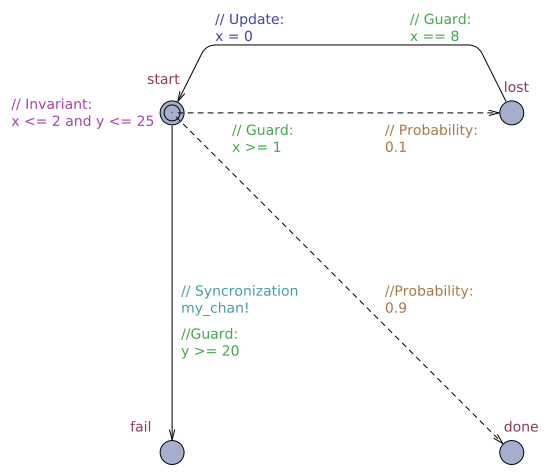
\includegraphics[height=3.4in, width=5in]{Figures/ptaExample.png}}
%\end{center}
%\begin{comment}\end{comment}  

%% \fcolorbox{frameColor}{white}{

% \newcommand{\frameImage}[3]{
% \begin{center}
%    \fcolorbox{frameColor}{white}{
%        \includegraphics[height=#2, width=#3]{#1} }
%\end{center}
%}
\usepackage{float}

\newcommand{\frameImage}[3]{
\begin{figure}[H] 
  \centerline{
    \fcolorbox{frameColor}{white}{
        \includegraphics[height=#2, width=#3]{#1} } }
    \caption{}
    \label{fig:#1}
\end{figure}
}

\usepackage[nomessages]{fp}

\newcommand{\frameImageRotate}[3]{
\begin{figure}[H] 
  \centerline{
    \FPeval\widthdim{7.8}
    \FPeval\heightdim{#2 / #3 * \widthdim}
    \fcolorbox{frameColor}{white}{
        \includegraphics[height= \heightdim in, width=\widthdim in, angle=270]{#1} } }
    \caption{}
    \label{fig:#1}
\end{figure}
}

\newcommand{\frameSvg}[3]{
\begin{figure}[H] 
    \input{#1}
    \caption{}
    \label{fig:#1}
    
  
\end{figure}
}

\newcommand{\imageInTable}[3]{
\begin{center}
    \fcolorbox{frameColor}{white}{
        \includegraphics[height=#2, width=#3]{#1} }
\end{center}
}

%\fcolorbox{frameColor}{white}{
%\label{fig:figure_#1}

\newcommand{\tableImage}[4]{
  \begin{table}[H] 
    \setlength\tabcolsep{0pt}
    \centering 
    \begin{tabular}{c|c}
    \setlength\tabcolsep{0pt}
    #1 & #3 \\
    #2 & #4
    \end{tabular} 
  \end{table}
}

\usepackage{comment}
\usepackage{amssymb}
\usepackage{mathrsfs}

\newcommand{\out}[1]{\ignorespaces}

\newcommand{\tmy}[2]{
$ #1 $
}

\newcommand{\tmz}[1]{
$ #1 $
}

\newcommand{\cstate}[1]{
\textit{\textcolor{ColorUppaalState}{#1}}
}

\definecolor{blue-green}{rgb}{0.0, 0.87, 0.87}
\definecolor{brightgreen}{rgb}{0.4, 1.0, 0.0}
\definecolor{richblack}{rgb}{0.0, 0.25, 0.25}
\definecolor{blue(pigment)}{rgb}{0.2, 0.2, 0.6}
\definecolor{cardinal}{rgb}{0.77, 0.12, 0.23}

\usepackage{listings}

\lstdefinestyle{styleuppaal}{
  belowcaptionskip=1\baselineskip,
  breaklines=true,
  %frame=single,
  xleftmargin=\parindent,
  language=C,
  showstringspaces=false,
  basicstyle=\footnotesize\ttfamily,
  keywordstyle=\bfseries\color{blue(pigment)},
  morekeywords={bool,true,false,clock},
  commentstyle=\itshape\color{cardinal},
  identifierstyle=\color{richblack},
  stringstyle=\color{blue-green},
}


\newcommand\colorsCellHeight {12}
\newcommand\colorsCellWidth  {110}

\newcommand\colorsTable  {
\begin{table}[H] 
\centering 
\begin{tabular}{|l|c|c|} \hline
Attribute               & RGB(hexadecimal \#RRGGBB) & Color\\ \hline
Node Name               & \#8C3863                  & \fcolorbox{ColorNodeName}{ColorNodeName}{\makebox(\colorsCellWidth,\colorsCellHeight){}} \\ \hline
Node Invariant          & \#A742A8                  & \fcolorbox{ColorNodeInvariant}{ColorNodeInvariant}{\makebox(\colorsCellWidth,\colorsCellHeight){}} \\ \hline
Edge Guard              & \#42A848                  & \fcolorbox{ColorEdgeGuard}{ColorEdgeGuard}{\makebox(\colorsCellWidth,\colorsCellHeight){}} \\ \hline
Edge Probability        & \#A87A42                  & \fcolorbox{ColorEdgeProbability}{ColorEdgeProbability}{\makebox(\colorsCellWidth,\colorsCellHeight){}} \\ \hline
Edge Update             & \#4242A8                  & \fcolorbox{ColorEdgeUpdate}{ColorEdgeUpdate}{\makebox(\colorsCellWidth,\colorsCellHeight){}} \\ \hline
Edge Synchronization    & \#42A0A8                  & \fcolorbox{ColorEdgeSynchronization}{ColorEdgeSynchronization}{\makebox(\colorsCellWidth,\colorsCellHeight){}} \\ \hline
\end{tabular} 
\end{table}
}

\newcommand\runTimesPLPsTable  {
\begin{table}[H] 
\centering 
\begin{tabular}{|l|c|c|} \hline
PLP                        & Lower boundary & Upper boundary \\ \hline
achieve\_door\_open        &      100       &      200  \\ \hline
achieve\_door\_unlock      &      100       &      200  \\ \hline
achieve\_key\_take         &      100       &      200  \\ \hline
achieve\_move\_to          &      400       &      600  \\ \hline
maintain\_key\_hold        &       ?        &       ?   \\ \hline
observe\_is\_door\_locked  &      300       &      700  \\ \hline
observe\_is\_door\_open    &      300       &      1000 \\ \hline
\end{tabular} 
\end{table}
}

\usepackage{tabularx}

\newcommand\plpsExecutionTable  {
\begin{table}[H] 
\centering 
\begin{tabularx}{\linewidth}{|*{7}{>{\centering\arraybackslash}X|}} \hline
Path 1: & Path 2: & Path 3: & Path 4: \\
Parallel to other paths, makes sure that robot holding a key & In case the door is open  & In case the door is closed but unlocked &  In case the door is closed and locked \\ \hline
\multicolumn{4}{|c|}{move\_to(key)}  \\ \hline
\multicolumn{4}{|c|}{key\_take }     \\ \hline
\multirow{7}{*}{key\_hold} & \multicolumn{3}{c|}{move\_to(doorway)} \\ \cline{2-4}
& \multicolumn{3}{c|}{is\_door\_open}  \\ \cline{2-4}
& \multirow{4}{*}{\shortstack{move\_to \\ (through\_doorway)}} & \multicolumn{2}{c|}{is\_door\_locked}   \\ \cline{3-4}
& & \multirow{2}{*}{door\_open} & door\_unlock  \\ \cline{4-4} 
& & & door\_open  \\ \cline{3-4} 
& & move\_to (through\_doorway) & move\_to (through\_doorway) \\ \cline{2-4} 
& move\_to(target) & move\_to(target) & move\_to(target)  \\ \hline 
\end{tabularx} 
\end{table}
}

\newcommand\queriesTable  {
\begin{table}[H] 
\centering 
\begin{tabularx}{\linewidth}{|*{4}{>{\centering\arraybackslash}X|}} \hline

Name                    & Property                                          & Explanation                                                                       & Equivalent to                             \\ \hline
Possibly                & \textit{E<> p}                                    & If exist a path that \textit{p} is eventually true.                               &                                           \\ \hline
Invariantly             & \textit{A\small[\small] p}                        & If for all paths \textit{p} is true all the time.                                 & \textit{not E<> not p}                    \\ \hline
Potentially always      & \textit{E\small[\small] p}                        & If exist a path that \textit{p} is true all the time.                             &                                           \\ \hline
Eventually              & \textit{A<> p}                                    & If for all the paths, \textit{p} is eventually true.                              & \textit{not E\small[\small] not p}        \\ \hline
Leads to                & \textit{p - -> q}                                 & For all the paths, if \textit{p} is true, \textit{q} will be eventually true.     & \textit{A\small[\small] (p imply A<> q)}  \\ \hline
Probability eventually  & \textit{Pr\small[\small] (<>q)}                   & Calculate the probability of \textit{q} eventually true.                          &                                           \\ \hline
Probability always      & \textit{Pr\small[\small] (\small[\small]q)}       & Calculate the probability of \textit{q} always true.                              &                                            \\ \hline

\end{tabularx} 
\end{table}
}



\newcommand\runTimesPTAsTableAll  {
\begin{table}[H] 
\centering 
\begin{tabular}{l l}
\underline{PLP}		& \underline{Run time range}    \\
move\_to(key)		& [400,600]     \\
key\_take 		   	& [100,200]     \\
move\_to(doorway) 	& [400,600]     \\
is\_door\_open		& [300,1000]    \\
is\_door\_locked	& [300,700]     \\
door\_unlock		& [100,200]     \\
\end{tabular} 
\end{table}
}

\newcommand\runTimesPTAsTableStart  {
\begin{table}[H] 
\centering 
\begin{tabular}{l l} 
\underline{PLP} & \underline{Run time range}  \\
move\_to(key) 	  & [400,600] \\
key\_take 	  	 & [100,200]  \\
\end{tabular} 
\end{table}
}



\newcommand\tab{\hspace{1cm}}

\usepackage{color,soul}

\definecolor{chartreuse(web)}{rgb}{0.5, 1.0, 0.0}
%\sethlcolor{chartreuse(web)}

% \begin{lstlisting}[style=styleuppaal]
% \lstset{escapechar=@,style=customc}

\definecolor{darkmidnightblue}{rgb}{0.0, 0.2, 0.4}
\definecolor{darkcerulean}{rgb}{0.03, 0.27, 0.49}
\definecolor{oxfordblue}{rgb}{0.0, 0.13, 0.28}
\definecolor{smokyblack}{rgb}{0.06, 0.05, 0.03}

\usepackage{hyperref} 

\hypersetup{
    colorlinks=true,
    linkcolor=smokyblack,
    filecolor=magenta,      
    urlcolor=blue,
    citecolor=darkcerulean,
}
\urlstyle{same}

\def\changemargin#1#2{\list{}{\rightmargin#2\leftmargin#1}\item[]}
\let\endchangemargin=\endlist 


\definecolor{gray}{rgb}{0.4,0.4,0.4}
\definecolor{darkblue}{rgb}{0.0,0.0,0.6}
\definecolor{cyan}{rgb}{0.0,0.6,0.6}

\lstdefinestyle{stylexml}{
  basicstyle=\ttfamily,
  columns=fullflexible,
  breaklines=true,
  showstringspaces=false,
  commentstyle=\color{gray}\upshape
}

\lstdefinelanguage{XML}
{
  morestring=[b]",
  morestring=[s]{>}{<},
  morecomment=[s]{<?}{?>},
  stringstyle=\color{black},
  identifierstyle=\color{darkblue},
  keywordstyle=\color{cyan},
  morekeywords={xmlns,version,type}% list your attributes here
}


\definecolor{purple(munsell)}{rgb}{0.62, 0.0, 0.77}

%%%%%%%%%%%%%%%%%%%%%%%%%%%%%%%%%%%%%%%%%%%%%%%%%%%%%%%%%%%%%%%%%
%% ACTUAL DOCUMENT.
%%%%%%%%%%%%%%%%%%%%%%%%%%%%%%%%%%%%%%%%%%%%%%%%%%%%%%%%%%%%%%%%%

\begin{document}

% Use Roman numerals (i, ii, iii, etc.) for page numbers in the front matter.


%%\pagenumbering{roman}
\frontmatter

%%%%%%%%%%%%%%%%%%%%%%%%%%%%%%%%%%%%%%%%%%%%%%%%%%%%%%%%%%%%%%%%%
%% TITLE PAGE.
%%%%%%%%%%%%%%%%%%%%%%%%%%%%%%%%%%%%%%%%%%%%%%%%%%%%%%%%%%%%%%%%%

% No headers or footers on the title page.
\thispagestyle{empty}

\begingroup
\centering
\setstretch{1.0}
~
\\[1em]
\sffamily\bfseries\fontsize{26}{31.2}\selectfont
\DocumentTitle
\\[0.4in]
\normalfont\large
Thesis by
\\[0.25em]
\sffamily\bfseries\Large
\AuthorName
\\[0.15em]
\normalfont\normalsize
\href{mailto:alex.cs.rnd@gmail.com}{alex.cs.rnd@gmail.com}
\\[0.4in]
\normalfont\large
Supervised by
\\[0.25em]
\sffamily\bfseries\Large
Ronen I. Brafman
\\[0.15em]
\normalfont\normalsize
\href{mailto:brafman@cs.bgu.ac.il}{brafman@cs.bgu.ac.il}
\\[0.4in]
\normalfont\normalsize
In Partial Fulfillment of the Requirements
\\[0.5em]
for the Degree of
\\[0.5em]
Master of Science
\\[0.5em]
in
\\[0.5em]
Computer Science
\vfill
\includegraphics[height=1.8in, width=1.8in]
{bengurion.png}
\\[1.5em]
Ben-Gurion University of the Negev
\\[0.5em]
Beer Sheva, Israel
\\[1.5em]
October 2017
\par
\endgroup



\setcounter{page}{1}
\pagestyle{plain}
\cleardoublepage

\pagestyle{plain}





%\newpage
%\thispagestyle{empty}
%\null
%\newpage


%%%%%%%%%%%%%%%%%%%%%%%%%%%%%%%%%%%%%%%%%%%%%%%%%%%%%%%%%%%%%%%%%
%% COPYRIGHT PAGE.
%%%%%%%%%%%%%%%%%%%%%%%%%%%%%%%%%%%%%%%%%%%%%%%%%%%%%%%%%%%%%%%%%

%\pagestyle{plain}

%\setcounter{page}{2}
\begingroup
\centering
\setstretch{1.0}
\null
\vfill
{\sffamily\textcopyright}~2017
\\[0.5em]
\AuthorName
\\[0.5em]
All Rights Reserved
\par
\endgroup


%%%%%%%%%%%%%%%%%%%%%%%%%%%%%%%%%%%%%%%%%%%%%%%%%%%%%%%%%%%%%%%%%
%% DEDICATION PAGE.
%%%%%%%%%%%%%%%%%%%%%%%%%%%%%%%%%%%%%%%%%%%%%%%%%%%%%%%%%%%%%%%%%

\begingroup
\centering
\setstretch{1.0}
~
\\[1in]
\textit{}
\par
\endgroup

\cleardoublepage

%%%%%%%%%%%%%%%%%%%%%%%%%%%%%%%%%%%%%%%%%%%%%%%%%%%%%%%%%%%%%%%%%
%% ABSTRACT.
%%%%%%%%%%%%%%%%%%%%%%%%%%%%%%%%%%%%%%%%%%%%%%%%%%%%%%%%%%%%%%%%%

\chapter*{Abstract}
\addcontentsline{toc}{chapter}{Abstract}

%%% ABSTRACT_REPLACE_START %%%

\textit{Performance Level Profiles} (PLPs) were developed as a formal, quantitative language for specifying the behavior of functional modules. There are four types of PLPs: 1. Achieve - achieves internal and external goals. 2. Observe - senses environment. 3. Maintain - maintains a property. 4. Detect - detects property. In this thesis, we propose a formal way to represent all the PLPs in terms of \textit{Probabilistic Timed Automatons} (PTAs). To go beyond single module level we define a \textit{control graph} as a formal representation of execution plan for robotic modules specified by PLPs, enhanced with probabilities, conditional branching, parallel execution etc. Finally, we developed software that compiles PLPs specification and \textit{control graph} plan into a single system suitable for offline analysis by UPPAAL model checker.\\

%%% ABSTRACT_REPLACE_END %%%

%%%%%%%%%%%%%%%%%%%%%%%%%%%%%%%%%%%%%%%%%%%%%%%%%%%%%%%%%%%%%%%%%
%% TABLE OF CONTENTS (TOC), LISTS OF FIGURES, TABLES, ETC.
%%%%%%%%%%%%%%%%%%%%%%%%%%%%%%%%%%%%%%%%%%%%%%%%%%%%%%%%%%%%%%%%%

\tableofcontents

%%\listoffigures

%%\listoftables

\cleardoublepage

% Use Arabic numerals (1, 2, 3, etc.) for subsequent page numbers.
%%\pagenumbering{arabic}
\mainmatter


%%\input{Thesis-Chapter-Intro.tex}

\chapter{Introduction}
In recent years, we are witnessing accelerated development in the field of autonomous robotic systems. There are many possible applications for autonomous robots, and each application introduces new challenges. Especially challenging is the development of autonomous robots functioning alongside humans in a safe and reliable manner. Hence the growing need for methods for building reliable and predictable autonomous robots. Currently, there are a few existing tools \cite{basu2008incremental} that seek to achieve these goals by defining formal programming languages for describing a robotic system that generates code with various guarantees and support the ability to prove and infer system properties. Unfortunately, these tools have not been widely adopted, and most developers prefer to use regular programming languages to design robotic components.
\par One of the key problems with code written using standard programming languages is that it is not always clear what level of performance one can expect from it. Such information is required to understand what one can expect from a robot using such code. It is essential information for predicting its behavior and is required to enable appropriate reuse of code. This information can sometimes be obtained from its documentation, but the standard specification techniques used by most software engineers are informal, qualitative, and use free text which is not machine readable. 
\par \textit{Performance Level Profiles} (PLPs) \cite{brafman2014performance} \cite{brafman2016performance} were developed as a formal, quantitative language for specifying the behavior of functional modules. PLPs were developed to help developers who use regular programming languages provide a formal, quantitative, machine readable specification of their module’s behavior. This information makes it possible to reuse the abundant existing modules more reliably and also makes possible automatic analysis, monitoring of modules, as well the use of automated learning techniques to update their descriptions. PLPs can be used by a robotic control unit to provide it with information about conditions needed to execute a module, conditions made true by the module when done successfully, possible failure modes, the module’s probability to complete its work successfully without any failure, time distribution of its execution, and more.
\par There are four types of PLPs: 1. Achieve - works to achieve some desirable property, internal or external. 2. Observe - attempts to reveal a value of an environmental variable. 3. Maintain - works to keep a certain variable in particular range or maintain some condition while running. 4. Detect - attempts to identify some condition that is either not true now, or that is not immediately observable. 
\par Generally, PLPs provide a basis to look at a software module as a sort of logical unit that can be executed only if its preconditions are satisfied, and when executed it achieves certain goals. Elements used by PLPs can provide a foundation for modular system design and other complex applications. Currently, software tools for PLPs \cite{brafman2016performance} are used to: 1. Generate code automatically from a PLP to monitor conditions specified by the PLP 2. Analyze performance to update the PLP specification. 3. Generate plans that achieve user specified tasks on the fly, by both generating domains descriptions that can be used in off-the-shelf planners, and also providing the needed software interfaces between the planner and the underlying functional module.
\par But while PLPs are quite intuitive, they lack a formal semantics. Such semantics is essential to make their meaning clear and is required to be able to prove properties. Moreover, a robot’s behavior is the result of the execution of multiple modules combined in diverse ways, and one would want to go beyond the module level in order to characterize and prove properties of the entire program. The goal of this thesis is to address these problems theoretically and practically. 
\par In this thesis, we propose a formal semantics for PLP defined by \textit{Probabilistic Timed Automaton} (PTA) \cite{norman2013model}, on which we apply then an existing model checking tool. We introduce a structure, \textit{control graph}, which represents a control unit of a robot that uses PLPs as functional units. We show how \textit{control graphs} and PLPs can be used to verify properties of the whole system offline, and we provide a software tool implementing this technique.
\par Any formal model of PLPs must incorporate some elements that are an essential part of PLPs. More specifically, we want a model that can represent and use: numbers, numerical variables, numerical comparisons, logical conditions, time progress, distribution of run time, and probabilistic transitions and events. The simplest model we found that captures these aspects while providing sufficiently mature model checking tool and clear semantics is \textit{Probabilistic Timed Automaton} (PTA) \cite{norman2013model}.
\par A \textit{Probabilistic Timed Automaton} (PTA) is a type of finite hybrid automata extended with probabilities. PTA uses real-valued variables called \textit{clocks} that increase simultaneously at the same rate. PTA transitions can contain logical conditions on boolean or \textit{real} variable, \textit{clocks} comparison to \textit{real} values, and branch points with probabilities on each transition. With a PTA description of a system, we can ask certain types of questions about the system. Typical questions are: 1. Reachability - whether a certain state could be reached by some valid execution path. 2. Safety - whether certain condition always holds. 3. Liveness - whether a specific condition holds eventually. 4. Deadlock - is deadlock possible or not. All the questions above can be addressed with model checking algorithms on a PTA model. We use UPPAAL \cite{uppaalIntroduction} \cite{tutorialUppaal} as our model checking tool, due to its support of all the essential features.
\par We use PTA qualities ( logical conditions, \textit{clocks}, and probabilities ) to create a single PTA template for each PLP type thus providing it with a semantic model. Each specific PLP instance of each type will be represented by an automaton with unique conditions, effects, time distributions, probabilities and goals, which constitute an instantiation of the general PTA schema for the corresponding PLP type. 
\par But we want to go beyond the level of a single functional module. We would like to be able to use the above semantics to verify the properties of complex behaviors that involve multiple functional modules executed in complex ways. But if we want to address bigger problems that require complex robotic behavior, dealing with individual models is not enough. Usually, such behavior is not a mere sequence of execution of modules, but an algorithm or program that we refer to as a robotic controller, or controller, for short. A controller controls the robot and schedules the execution of particular modules. We assume that the controller can access robot’s sensors and more generally any robotic module attached to it. Such a controller is usually designed with some goal in mind.
\par Usually, a controller works directly with specific robotic modules through a custom interface and without a standard technique for analysis, monitoring, and logging. This practice limits the opportunities for reusability of modules and automation of the system. We can address these limitations by using a PLP based interface between the controller and actual robotic module. We will define a \textit{control graph} as a general description of a robotic controller that will use a PLP based interface to control robotic modules. 
\par The \textit{control graph} describes controller algorithms. It is very similar to decision trees in structure, enhanced with multiple execution paths and nodes that function as intersections of execution paths that fuse into a single path. \textit{Control graphs} can use variables shared with PTAs representing certain PLPs, to provide input arguments to PTAs and to receive outputs from them. The \textit{control graph} uses conditions and probabilities to determine the execution sequence of PTAs representing PLPs. A \textit{control graph} is built from 4 elementary nodes: 1. \textit{Sequential node} - executes a sequence of PLPs. 2. \textit{Probabilistic node} - has multiple outgoing edges, each with probability to be executed. 3. \textit{Conditional node} - outgoing edges have conditions, and only a single edge with a true condition can be executed. 4. \textit{Concurrent node} - all the outgoing edges are scheduled at the same time and executed concurrently. 
\par \textit{Control graphs} and PLPs are the inputs to our software tool. Each node of a \textit{control graph} is compiled into a PTA: 1. A \textit{sequential node} schedules the execution of PLPs by the defined sequence, waiting for each PLP to finish. 2. Probabilistic and \textit{conditional nodes} use PTAs’ edges with probabilities and conditions. 3. \textit{Concurrent node} schedules execution of multiple subsequent nodes, according to the outgoing edges. After the compilation of \textit{control graph} and PLPs to a network of PTAs, we use the UPPAAL model checker to query the whole system. The designer of a controller could use results of our compilation as a way to verify that the system would work as he expects it to work. In particularly the designer can verify that certain states are reachable, and estimate whether the probabilities to reach those states are acceptable. Conclude the final goal of this thesis.
\par Contributions:
\begin{itemize}
\item An introduction of formal semantics for PLPs with \textit{Probabilistic Timed Automaton} templates representation for each PLP type. This semantics capture the aspects of PLPs: logical premises, probabilistic outcomes, and temporal distributions. Furthermore, we introduce a mechanism for the enforcement of \textit{concurrent conditions}.
\item An introduction and formalization of \textit{control graph} as a relatively simple way to represent robotic controllers and algorithms, based on robotic modules specified by PLPs.
\item A verification method of a system combining \textit{control graphs} and PLPs by conversion of the system to a network of PTAs and using a model checker on it. Including working implementation in Java.
\end{itemize}
\chapter{Background}
\section{\textit{Performance Level Profiles}}
\textit{Performance Level Profiles} serve as agreements between robotic module designers and systems that use it. PLPs describe the conditions under which a module should be operated, its expected run time and probabilities of success and failures. PLPs were designed with rigid and machine-readable syntax, with the following objectives in mind: 1. Automated analysis, monitoring, and reuse of existing code. 2. Convey to customers a certain expected level of performance of an autonomous robot. 3. Quickly identify an abnormal behavior of autonomous robots. Currently, there are four types of PLPs: Achieve, Maintain, Observe and Detect. They share common characterizations but differ in the purposes of the modules they represent.\\
\subsection{Common elements \label{plp_common_elements}}
\begin{itemize}
\item Parameters - input and output variables used by the module.
\item Required resources - list of resources and quantities (if needed).
\item Preconditions - conditions involving parameters that must be satisfied for the module to be executed.
\item \textit{Concurrent conditions} - conditions on variables that must be satisfied while the current module is being executed.
\item \textit{Concurrent module}s - conditions on other modules that must or must not be executed at execution time of the current module.
\item Parameter frequency (optional) - the frequency of reading or writing of variables.
\item Side-effects - unintended effect of a running module, described by a conditional assignment to a parameter. For example consumption of power resource.
\item Expected progress rate - expected rate of completing the task.
\end{itemize}
\subsection{\textit{PLP Achieve} \label{plp_achieve}}
Achieve modules want to accomplish some desirable property. That can be either an external state of the world or internal virtual property. An example for an external goal for Achieve module is to reach world state in which the fuel tank is full. An example of an internal Achieve module is to generate a path to a certain destination.\\
Additional elements:
\begin{itemize}
\item Goal - a boolean condition that is achieved by the module.
\item Failure modes - possible failure cases.
\item Success probability.
\item Failure modes probability.
\item Run time distribution - for success and failure modes.
\end{itemize}
\subsection{\textit{PLP Maintain}  \label{plp_maintain}}
Maintain modules keep the value of a variable at a certain value or the truth value of some condition. The maintained conditions can be false at the beginning, and it may need some time to become true. Maintain module can be used for example to maintain a certain speed or maintain direction.\\
Additional elements:
\begin{itemize}
\item Maintained condition - condition to be maintained by the module.
\item Whether the maintained condition is initially true. 
\item \textit{Termination condition} for success.
\item \textit{Termination conditions} for failure modes.
\item Success probability.
\item Failure modes probability.
\item Run time distribution - for success and failure modes.
\end{itemize}
\subsection{\textit{PLP Observe} \label{plp_observe}}
Observe type of module attempt to reveal the value of some variable or boolean condition. For example, observe whether the robot is standing.\\
Additional elements:
\begin{itemize}
\item Observation goal - boolean condition to be verified or a parameter whose value is to be observed.
\item Success probability.
\item Failure to observe probability.
\item Run time distribution - for success and failure modes.
\end{itemize}
\subsection{\textit{PLP Detect} \label{plp_detect}}
Detect modules try to identify some condition that is either not true now, or that is not immediately observable. For example, intruder detection or detect an obstacle.\\
Additional elements:
\begin{itemize}
\item Detect goal - the condition being detected.
\item Success probability.
\end{itemize}
\subsection{Repeat \label{plp_repeat}}
Repeat is an extension made for modules that should be run continuously, to repeat a certain task. Repeat can be used with \textit{PLP Achieve} and \textit{PLP Observe} that should be executed repeatedly in certain frequency until its \textit{termination condition} becomes true. Instead of hiding the repetitions inside the module, repeat make possible to control the repetition parameters: 1. \textit{Execution frequency} - how many times the module is executed per unit time. 2. Input frequency - minimal expected update frequency of variables. 3. Repeat \textit{termination condition} - the condition that stops the repeat of a module.\\
\section{Probabilistic Timed Automata (PTAs)}
Probabilistic timed automata (PTAs) are a formalism for modeling systems whose behavior incorporates both probabilistic and real-time characteristics. \cite{norman2013model} \cite{kwiatkowska2009stochastic}\\
\subsection{Time and \textit{clocks}}
Probabilistic timed automata model time using \textit{\textit{clocks}}, variables over the set \tmy{ \mathbb{R}_{\geqslant 0} }{ℝ≥0} of non-negative \textit{reals}. We assume a finite set \tmy{\mathscr{X}}{𝒳} of \textit{clocks}. A function \tmy{v:\mathscr{X}\rightarrow\mathbb{R}_{\geqslant 0}}{v : 𝒳 $\rightarrow$ ℝ≥0} is referred to as a \textit{clock} \textit{valuation} and the set of all \textit{clock} valuations is denoted by \tmy{\mathbb{R}^{\mathscr{X}}_{\geqslant 0}}{ℝ≥0𝒳 }. For any \tmy{ v \in \mathbb{R}^{\mathscr{X}}_{\geqslant 0}}{v $\in$ ℝ≥0𝒳}, \tmy{ t \in \mathbb{R}_{\geqslant 0}}{t $\in$ ℝ≥0} and \tmy{ X \subseteq \mathscr{X}}{X ⊆ 𝒳 }, we use \tmy{v+t}{v+t} to denote the \textit{clock} valuation which increments all \textit{clock} values in \tmy{v}{v} by \tmy{t}{t} and \tmy{v[X:=0]}{v[X:=0]} for the valuation in which \textit{clocks} in \tmy{X}{X} are reset to 0. \\
The set of \textit{clock} constraints over \tmy{\mathscr{X}}{𝒳} , denoted \tmy{CC(\mathscr{X})}{CC( 𝒳 )}, is defined by the syntax: \begin{center} \tmy{\chi ::= true $\vert$ x \leqslant d $\vert$ c \leqslant x $\vert$ x+c \leqslant y+d $\vert$ \neg \chi $\vert$ \chi \wedge \chi}{ χ ::= true $\vert$ x ≤ d $\vert$ c ≤ x $\vert$ x+c ≤ y+d $\vert$ ¬χ $\vert$ χ ∧ χ}\end{center}
where \tmy{ x,y \in \mathscr{X}}{x, y $\in$ 𝒳} and \tmy{ c,d \in \mathbb{R}}{c, d $\in$ ℝ}. A \textit{clock} valuation \tmy{v}{v} satisfies a \textit{clock} constraint \tmy{\chi}{χ}, denoted by \tmy{v \vDash \chi}{v |= χ}, if \tmy{\chi}{χ} resolves to true when substituting each occurrence of \textit{clock} x with \tmy{v(x)}{v(x)}. \textit{Clock} constraints will be used in the syntactic definition of PTAs and for the specification of properties.\\
\subsection{PTA Syntax}
A \textit{Probabilistic Timed Automaton} (PTA) is a tuple \tmy{P = ( L, l_0, \mathscr{X}, Act, inv, enab, prob )}{P = ( 𝐿, 𝑙0, 𝒳, Act, inv, enab, prob )} where: \\
– \tmy{L}{𝐿} is a finite set of locations and \tmy{l_0 \in L}{𝑙0 $\in$ 𝐿} is an \textit{initial location}; \\
– \tmy{\mathscr{X}}{𝒳} is a finite set of \textit{clocks}; \\
– \tmy{Act}{Act} is a finite set of \textit{actions}; \\
– \tmy{inv : L \rightarrow CC(\mathscr{X})}{inv : 𝐿$\rightarrow$CC( 𝒳 )} is an \textit{\textit{invariant condition}}; \\
– \tmy{enab : L \times Act\rightarrow CC(\mathscr{X})}{enab : 𝐿×Act$\rightarrow$CC( 𝒳 )} is an \textit{enabling condition}; \\
– \tmy{prob : L \times Act \rightarrow Dist(2^\mathscr{X}\times L)}{prob : 𝐿×Act$\rightarrow$Dist( 2𝒳 × 𝐿 )} is a (partial) \textit{\textit{probabilistic transition function}}.
\par A state of a PTA is a pair \tmy{(l,v)\in L \times \mathbb{R}^\mathscr{X}_{\geqslant 0}}{(l, v) $\in$ L×ℝ𝒳 }such that \tmy{v \vDash inv(l)}{v |= inv(l)}. In any state \tmy{(l,v)}{(l, v)}, either a certain amount of time \tmy{t \in \mathbb{R}_{\geqslant 0}}{t $\in$ ℝ≥0} elapses or an action \tmy{a \in Act}{a $\in$ Act} is performed. If time elapses, then the choice of \tmy{t}{t} requires that  the invariant \tmy{inv(l)}{inv(l)} remains continuously satisfied while time passes. Each action \tmy{a}{a} can be only chosen if it is enabled, that is, the condition \tmy{enab( l, a )}{enab( l, a )} is satisfied by \tmy{v+t}{v+t}. Once action \tmy{a}{a} is chosen, a set of \textit{clocks} to reset and successor location are selected at random, according to the distribution \tmy{prob( l, a )}{prob( l, a )}. We call each element \tmy{( X, l' ) \in 2^\mathscr{X}\times L}{( X, l' ) $\in$ 2𝒳 × L} in the support of \tmy{prob( l, a )}{prob( l, a )} an edge and, for convenience, assume that the set of such edges, denoted \tmy{edges( l, a )}{edges( l, a )}, is an ordered list \tmy{ \left \langle e_1, \ldots , e_n \right \rangle }{〈 e1, . . . , en〉}.
\par We assume that PTAs are well-formed, meaning that, for each state \tmy{(l,v)}{( l, v )} and action \tmy{a}{a} such that \tmy{v}{v} satisfies \tmy{enab( l, a )}{enab( l, a )}, every edge \tmy{( X, l' ) \in edges( l, a )}{( X, l' ) $\in$ edges( l, a )} results in a transition to a valid state, i.e., we have \tmy{v[X:=0] \vDash inv( l' )}{v[X:=0] |= inv( l' )}. A PTA can be transformed into one that is well-formed by incorporating the invariant associated with the target location into the \textit{enabling condition} of each location-action pair \cite{kwiatkowska2007symbolic}.\\
\subsection{PTA Semantics}
Let \tmy{P = ( L, l_0, \mathscr{X}, Act, inv, enab, prob )}{P=(L, 𝑙0, 𝒳, Act, inv, enab, prob)} be a PTA. The semantics of P is defined as a tuple \tmy{( S, s_0, Act \times \mathbb{R}_{\geqslant 0} , Steps_P )}{( S, s0, Act × ℝ, StepsP )} where: \\
– A probability distribution function \tmy{\mu}{µ}.\\
– Set of states \tmy{S = \left \{ ( l, v ) \in L \times \mathbb{R}^\mathscr{X}_{\geqslant 0} \mid  v \vDash inv( l ) \right \}}{S = { ( l, v ) $\in$ L × ℝ𝒳 $\vert$ v |= inv( l ) }} and initial state \tmy{s_0 = ( l_0 , \mathbf{0} )}{s0 = ( 𝑙0, 0 )}; \\
– for any \tmy{( l, v ) \in S}{( l, v ) $\in$ S} and \tmy{a \in Act \cup \mathbb{R}_{\geqslant 0}}{a $\in$ Act ∪ ℝ≥0}, we have \tmy{Steps_P ( ( l, v ), a ) = \lambda}{StepsP ( ( l, v ), a ) ) = λ} if and only if either:\\
Time transitions. \tmy{a \in \mathbb{R}_{\geqslant 0}, v + t' \vDash inv(l)}{a $\in$ ℝ≥0, v + t' |= inv(l)} for all \tmy{0 \leqslant t' \leqslant a}{0 ≤ t' ≤ a} and \tmy{\lambda = \mu_{( l,v+a)}}{λ = µ( l,v+a)};\\
Action transitions. \tmy{a \in Act, v \vDash enab( l,a )}{a $\in$ Act, v |= enab( l,a )} and for each \tmy{( l',v' ) \in S}{( l',v' ) $\in$ S}: \begin{center} \tmy{\lambda (l' , v' ) = \sum \left \{ \mid prob( l, a )(X, l' ) \mid X \in 2^\mathscr{X} \land v' = v[X:=0] \mid \right \}}{λ( l' , v' ) = 𝛴 {| prob( l, a )(X, l' )| X $\in$ 2𝒳 ∧ v' = v[X:=0] |}}. \end{center}
\section{PTA augmentations}
We now summarize a variety of extensions to the standard definition of PTAs that facilitate high-level modeling using this formalism. \\
\subsection{Parallel composition}
It is often useful to define complex systems as the \textit{parallel composition} of several interacting components. The definition of the \textit{parallel composition} operator \tmy{\parallel}{‖} for PTAs \cite{kwiatkowska2003probabilistic} uses ideas from (untimed) probabilistic automata \cite{segala1995probabilistic} and classical timed automata \cite{alur1994theory}. Let \tmy{P_i = ( L_i, \bar{l}_i, \mathscr{X}_i, Act_i, inv_i, enab_i, prob_i )}{Pi = ( 𝐿i, l'i, 𝒳i, Acti, invi, enabi, probi )} for \tmy{i \in{1,2}}{i $\in$ {1,2}} and assume that \tmy{\mathscr{X}_1 \cap \mathscr{X}_2 = \emptyset }{𝒳1 ∩ 𝒳2 = Ø} . Given \tmy{\mu_1 \in Dist(2^{\mathscr{X}_1} \times L_1 ) }{µ1 $\in$ Dist(2𝒳1 ×L1)} and \tmy{\mu_2 \in Dist(2^{\mathscr{X}_2} \times L_2 ) }{µ2 $\in$ Dist(2𝒳 2×L2)}, we let \tmy{ \mu_1 \bigotimes \mu_2 \in Dist(2^{\mathscr{X}_1 \cup \mathscr{X}_2} \times (L_1 \times L_2 ) ) }{µ1⊗µ2 $\in$ Dist(2𝒳 1∪𝒳 2 × (L1×L2))} be such that \tmy{\mu_1 \bigotimes \mu_2 (X_1 \cup X_2, (l_1,l_2)) = \mu_1(X_1,l_1) \cdot \mu_2(X_2,l_2) }{µ1⊗µ2(X1 ∪ X2,(l1,l2)) = µ1(X1,l1)·µ2(X2,l2)} for \tmy{X_i \subseteq \mathscr{X}_i, l_i \in L_i }{Xi ⊆ 𝒳i, li $\in$ Li } and \tmy{ i \in \left \{1,2 \right \}}{ i $\in$ {1,2}}. The \textit{parallel composition} of PTAs \tmy{P_1}{P1} and \tmy{P_2}{P2} is the PTA: \begin{center} \tmy{P_1\parallel P_2 = (L_1 \times L_2, (\bar{l}_1,\bar{l}_2), \mathscr{X}_1 \cup \mathscr{X}_2, Act_1\cup Act_2, inv, enab, prob )}{P1‖P2 = (L1×L2, (l'1,l'2), 𝒳1 ∪ 𝒳2, Act1∪Act2, inv, enab, prob ) } \end{center}
such that, for each location pair \tmy{(l_1,l_2) \in L_1 \times L_2}{(l1,l2) $\in$ L1×L2} and action \tmy{a \in Act_1\cup Act_2}{a $\in$ Act1∪ Act2}: 
\begin{itemize}
\item the \textit{\textit{invariant condition}} is given by \tmy{inv(l_1,l_2) = inv_1(l_1) \land inv_2(l_2)}{inv(l1,l2) = inv1(l1)∧inv2(l2)}; 
\item the \textit{enabling condition} is given by: 
\end{itemize}
\begin{center}\tmy{enab((l_{1},l_{2}),a) = \left\{\begin{matrix} enab_{1}(l_{1},a) \land enab_{2}(l_{2},a) & \textrm{if } a \in Act_{1} \cap Act_{2} \\ enab_{1}(l_{1},a) & \textrm{if } a \in Act_{1} \setminus Act_{2} \\ enab_{2}(l_{2},a) & \textrm{if } a \in Act_{2} \setminus Act_{1} \end{matrix}\right. }{}  \end{center} \newline   
\begin{itemize}
\item the \textit{\textit{probabilistic transition function}} is given by:  
\end{itemize}
\begin{center} \tmy{prob((l_{1},l_{2}),a) = \left\{\begin{matrix} prob_{1}(l_{1},a) \bigotimes prob_{2}(l_{2},a) & \textrm{if }  a \in Act_{1} \cap Act_{2} \\ prob_{1}(l_{1},a) \bigotimes \mu_{(\emptyset,l_2)} & \textrm{if } a \in Act_{1} \setminus  Act_{2} \\ \mu_{(\emptyset,l_1)} \bigotimes prob_{2}(l_{2},a) & \textrm{if } a \in Act_{2} \setminus Act_{1} \end{matrix}\right.}{} \end{center} \newline
\subsection{Variables}
When modeling systems with probabilistic timed automata, it is often convenient to augment the model with discrete variables \cite{behrmann2006uppaal} \cite{tri98}. For the sake of simplification of PLP to PTA conversion, we will use a stronger augmentation with an addition of real-valued variables. \textit{Enabling conditions} can then refer to the current value of the variables, and the probabilistic transition relation is extended to allow updating variable values. We add to the PTA definition a finite set of variables  \tmy{U}{U}, each variable can be evaluated with valuation function \tmy{\forall u \in U:  v(u) \in \mathbb{R}}{$\forall$u $\in$ U : v(u) $\in$ ℝ }. 
\par \textit{Enabling condition} is extended to contain \textit{variable constraints} additionally to \textit{clock} constraints \tmy{CC(\mathscr{X}) \wedge VC(U)}{CC(𝒳 )∧VC(U) }. \tmy{VC(U)}{VC(U)} is defined by the syntax: \begin{center} \tmy{\omega ::= true $\vert$ x \leqslant d $\vert$ c \leqslant x $\vert$ x+c \leqslant y+d $\vert$ \neg \omega $\vert$ \omega \wedge \omega}{ ω ::= true $\vert$ x ≤ d $\vert$ c ≤ x $\vert$ x+c ≤ y+d $\vert$ ¬ω $\vert$ ω ∧ ω}\end{center}
where \tmy{ x,y \in U}{x, y $\in$ U} and \tmy{ c,d \in R}{c, d $\in$ ℝ}.
\par \textit{\textit{Probabilistic transition function}}s are extended to include value update for a subset of variables. Variable is either updated to a result of a function depending on the subset of variables, or a probabilistic value corresponding to some distribution. \\
\subsection{Urgency}
When modeling real-time systems, it is often necessary to express the fact that a particular action should be taken immediately, without letting time pass. In this way, we can model, for example, an instantaneous system event comprising several atomic actions. A few mechanisms for modeling such situations have been introduced for timed automata, for example in the system-description language of the UPPAAL model checker \cite{behrmann2006uppaal}; here, we describe how they are adapted to PTAs. 
\par An \textit{urgent} location of a PTA is a location in which no time can pass. \textit{Urgent} locations can be represented in the PTA framework by introducing an additional \textit{clock}, which is reset on entry to an \textit{urgent} location, and by including a conjunct in the \textit{\textit{invariant condition}} of the location to specify that the value of the \textit{clock} should be equal to 0 in the location.\\
\subsection{Channels}
Channels are used to synchronize between two or more PTAs in a single \textit{parallel composition}. \\
The definitions of actions and \textit{parallel composition} can be extended to allow sending and receiving (to either single or multiple recipients) of messages along with them, as in UPPAAL \cite{behrmann2006uppaal}. Such behavior can be encoded in the action names of a standard PTA.\\
\section{PTA representation as graph}
PTAs can be represented in a much more compact and human-friendly form by a graphical representation, which preserves all the details of PTA semantics. Any instance of a PTA can be converted to unique PTA graph, and any PTA graph can be converted back to a PTA.\\
We will present how exactly the conversion from PTA semantic to PTA graph made and then we will be using a graphical representation for PTA.
\par For a PTA \tmy{P = ( L, l_0, \mathscr{X}, U, Act, inv, enab, prob )}{P = ( 𝐿, 𝑙0, 𝒳, U, Act, inv, enab, prob )}: \\
– \tmy{L}{𝐿} - \textit{locations} - each location represented by a node, with the same name. Initial location represented by a double outline on a single node. Time can pass only inside node;\\
– \tmy{\mathscr{X}}{𝒳 }- \textit{Clocks} - unchanged; \\
– \tmy{Act}{Act} - \textit{actions} - each action represented by a directed edge connecting two nodes, drawn as arrows; \\
– \tmy{inv}{inv} - \textit{\textit{invariant condition}} - represented as a condition located in attribute \textit{“invariant”} attached to a node. \textit{Invariant} can be omitted if true; \\
– \tmy{enab}{enab} - \textit{enabling condition} - represented by a condition located in attribute \textit{“guard”} attached to an edge. Guard can be omitted if true. Additionally to conditions involving \textit{clocks}, guard can also contain conditions involving variables; \\
– \tmy{prob}{prob} - \textit{\textit{probabilistic transition function}} - represented by a number in a range \small[0,1\small] located in attribute \textit{“probability”} attached to an edge. \textit{Probability} can be omitted if equal for all outgoing edges. Edges with omitted probabilities drawn by an arrow with continuous line, edges with non-omitted probabilities drawn by arrows with dashed lines. \\
– \textit{Clocks} resets and change of values for variables located in attribute \textit{“update”} attached to an edge. \textit{Update} is executed when action transition for a specific edge is being executed. Variable update with a probability according to a certain distribution would appear as a pattern: \tmy{variable\_name \in distribution()}{ variable_name $\in$ distribution()}.\\
– \textit{Urgent} locations - will be represented by “U” mark inside a node.\\
– Channels will be represented by a label with “?” or “!” sign located in attribute \textit{“synchronization”} attached to an edge. “!” - used by PTA sending a \textit{synchronization signal}. “?” - used by PTA receiving \textit{synchronization signal}. \\
– Run time distribution - will be part of the \textit{guard} attribute, it would appear as pattern: \tmy{clock\_name \in distribution()}{ \textit{clock}_name $\in$ distribution()}.\\
\section{PTA example}
Here we have a simple communication protocol represented with PTA. The PTA has two \textit{clocks} \textit{x} and \textit{y}, which start with the value 0. In the location \cstate{start}, the system waits for at least 1 time-unit (represented by the \textit{enabling condition} \tmy{x>=1}{x>=1} on the outgoing distribution of action send) and at most 2 time-units (represented by \tmy{x<=2}{x<=2} in the \textit{\textit{invariant condition}}), before sending a message. With probability 0.9 the message is received correctly (edge to \cstate{done}); otherwise, with probability 0.1, the message is lost (edge to \cstate{lost}). In the latter case, once \textit{clock} \textit{x} reaches 8, the PTA returns to \cstate{start} where another attempt to send the message can be made. If in total, at least 20 and at most 25 time-units have elapsed since the start of system execution, the PTA performs a timeout and moves to location \cstate{fail}. \frameImage{Figures/ptaExample.png}{3.22in}{4.02in}   
\par In the future graphical representations of PTAs, we will not be writing the role of each attribute; they will be close to node or edge they belong to, and color-coded:\\
\colorsTable
\chapter{Foundation for Formal Semantics for PLPs \label{foundation_for_formal_semantics_for_plps}}
We saw that there are four types of PLPs that describe four prototypes of robotic modules: Achieve, Maintain, Observe and Detect. All PLPs capture the three possible stages of robotic module execution: 1. Before execution - the parameters, resources, and conditions needed to run the module. 2. While executing - \textit{concurrent conditions}, and side effects. 3. After execution - a probability of success and failure, run time, and goal. We want to go over the specification of each type of PLP and create a representative PTA template, i.e., PTA\raisebox{-0.5ex}{\scriptsize{PLP}} that would embody PLP’s qualities such as run time distribution, a probability of success and failure, values changes of variables in a \textit{\textit{goal condition}}, etc. PTA\raisebox{-0.5ex}{\scriptsize{PLP}} is defined solely based on the information specificated in a PLP - the real underlying module, whether exists or not, is never used in the specification. In this section, we lay the foundation needed for PTA\raisebox{-0.5ex}{\scriptsize{PLP}} definitions. We will go through the individual components we use to transpose PLP into PTA\raisebox{-0.5ex}{\scriptsize{PLP}}.\\
\section{Variables}
All types of variables used by PLP, namely: parameters, variables, constants, and required resources are converted to real-valued variables of PTA. For boolean variables, false is defined as 0, and true as 1.\\
\section{Conditions \label{plp_to_pta_conditions}}
The term \textit{condition} is used in two different meanings in PLP: 1. The way we usually think of condition, for example, a PLP precondition: \textit{“a = b”} - meaning that if the value of \textit{a} equals value of \textit{b} then \textit{“a = b”} is true, but \textit{a} and \textit{b} do not have to be equal and the condition can be false. 2. As a statement that needs to be true and requires the variables to be adjusted accordingly. That is, as an indirect assignment statement. For example, the PLP \textit{\textit{goal condition}}: \textit{“a = b”} means that it must be true: Whatever the values of \textit{a} and \textit{b} were before; they must be equal to the same value at the end. Basically, the first meaning is a condition and the second meaning is an assignment of value. 
\par In the first case, to represent regular conditions, we use \textit{guard} attribute of a certain edge. \textit{Guard} attribute can contain: logical AND operators, logical NOT operators, comparison operator \textit{equal or smaller} (<=) on \textit{\textit{clocks}} and \textit{integers}. Comparison operator \textit{equal} (==) can be represented by: \textit{a == b iff (a <= b) AND (b <= a)}. Comparison operator \textit{equal or larger} (>=) can be represented by: \textit{a >= b iff (b <= a)}. Comparison operator \textit{larger} (>) can be represented by: \textit{a > b iff (b < a)}. Comparison operator \textit{smaller (<)} can be represented by: \textit{a < b iff (a <= b) AND NOT(a == b)}. Logical OR operator can be represented by using 2 edges, each one with a guard representing a different operand of logical OR.\\
To conclude, for a regular type of conditions in PLP we go over the conditions, possibly recursively, and produce the corresponding PTA\raisebox{-0.5ex}{\scriptsize{PLP}} \textit{guard}.
\par In the second case, condition as an assignment, we use an edge’s \textit{update} attribute, to assign a value to variables. The condition from PLP is translated to a series of assignments of values to variables. The condition of type \textit{“v == C”}, where \textit{v} is variable and \textit{C} is constant, translated into assignment \textit{“v $\leftarrow$ C”}. The condition of type \textit{“(C\raisebox{-0.5ex}{\scriptsize{1}} <= v) AND (v <= C\raisebox{-0.5ex}{\scriptsize{2}})”}, where v is variable and \textit{C\raisebox{-0.5ex}{\scriptsize{1}}, C\raisebox{-0.5ex}{\scriptsize{2}}} are constants, should produce the assignments: \textit{“v $\leftarrow$ C\raisebox{-0.5ex}{\scriptsize{1}}, v $\leftarrow$ C\raisebox{-0.5ex}{\scriptsize{1}}+1, …, v $\leftarrow$ C\raisebox{-0.5ex}{\scriptsize{2}} - 1, v $\leftarrow$ C\raisebox{-0.5ex}{\scriptsize{2}}”}, but assignments for the same variable with different values are meaningless if done in \textit{update} of single edge, therefore it will be split into multiple edges, each edge with single assignment into variable \textit{v} in its \textit{update}. Similarly, more complex conditions can be converted eventually into a set of assignments. \\
\section{Resources \label{plp_to_pta_resources}}
PLP can require certain resources to run, and optionally a minimum amount of them. We will define a single variable for each resource. PTA\raisebox{-0.5ex}{\scriptsize{PLP}} will check that there is enough of the resource. If an exclusive access to a resource required, we will check that it is indeed accessed by a single PLP.\\
\section{Preconditions \label{plp_to_pta_preconditions}}
Preconditions are conditions on variables required by PLP to run. We convert all the PLP type preconditions into PTA type conditions, then concentrate them as part of a \textit{guard} attribute at the beginning of every PTA\raisebox{-0.5ex}{\scriptsize{PLP}}.\\
\section{Goal \label{plp_to_pta_goal}}
The goal is accomplished when PLP is done successfully. We convert PLP goal into series of assignments into variables, at the end of successful completion of PTA\raisebox{-0.5ex}{\scriptsize{PLP}}.\\
\section{Success and failure probabilities \label{plp_to_pta_success_and_failure_probabilities}}
A PLP has a single success outcome and many possible failure outcome cases. Each possible outcome has a certain probability that represented with fraction between 0 to 1, the sum of all outcomes must be 1. We represent probabilities with probabilities on edges coming out from a single node. \\
\section{Side effects \label{plp_to_pta_side_effects}}
Side effects are the changes made to variables or resources by PLP during its execution. The two most significant complications caused by side effects: 1. Temporal - when exactly the side effects influence the variables: it can be a single point in time, multiple points in time, single interval or multiple intervals. 2. Value - the value that the side effect assigns to a variable can be constant or change according to time and other variables. Although PLP does not represent temporal nuances of side effects, we can be confident that side effects have been applied before the end of the PLP. We will make sure to enforce the update of the side effect at the end of representing PTA\raisebox{-0.5ex}{\scriptsize{PLP}}. \\
\section{\textit{Observed variable} \label{plp_to_pta_observed_variable}}
\textit{PLP Observe} is supposed to be able to obtain the value of a particular variable, as it appears in the environment. Although it is possible to model the environment of a robot, we decided not to over-complicate the system with an attempt to do so and to sustain a universal and probabilistic approach to the system. Therefore instead of just assigning a value from an environmental module, we use the domain of the specific \textit{observed variable} to choose its probable value. Currently, we use only a uniform probability on variable's domain, but this feature can be expanded in the future. \\
\section{Update attribute extension \label{plp_to_pta_update_attribute_extension}}
We will be using functions embedded inside the update attribute of an edge. A Function is basically a series of assignments to variables and \textit{clocks}, with an extension of conditional “\tmz{if}” statement. Conditional “\tmz{if}” statement evaluates a certain \tmz{if-condition}. If it is true, only the \tmz{true-part} is evaluated, if the condition is false, only the \tmz{false-part} is evaluated. “\tmz{if}” statement:\\
 \begin{center}\tmz{if ( if-condition ) \{ true-part \} else \{ false-part \}} \end{center}
A simple implementation of “\tmz{if}” statement, is to use two different edges with complementary parts of the “\tmz{if}” statement: 1. Edge with \tmz{if-condition} as a \textit{guard} attribute, and \tmz{true-part} as a content of an update attribute. 2. Edge with \tmz{NOT(if-condition)} as a \textit{guard} attribute, and \tmz{false-part} as a content of an update attribute.\\
For example, we create function check() that equals to: “\tmy{if ( 1 == a) \{ b \leftarrow 2, c \leftarrow 1  \} else \{ b \leftarrow 3, c \leftarrow 3 \}}{if ( 1 == a) { b $\leftarrow$ 2, c $\leftarrow$ 1  } else { b $\leftarrow$ 3, c $\leftarrow$ 3 }}”. If \tmz{a} equals 1 then \tmz{true-part} “\tmy{b \leftarrow 2, c \leftarrow 1}{b $\leftarrow$ 2, c $\leftarrow$ 1}” is executed, otherwise the \tmz{false-part} “\tmy{b \leftarrow 3, c \leftarrow 3}{b $\leftarrow$ 3, c $\leftarrow$ 3}” is executed. We can write: \frameImage{Figures/ptaTransitionCheck.png}{0.75in}{4.3in} Implementation: \\
\frameImage{Figures/ptaIfExample.png}{1.54in}{4.31in} Nested “\tmz{if}” statements can be implemented by attaching the nested conditions with logical AND into \textit{guard} attribute, and filling the update by response assignment of the most inner “\tmz{if}” (with an addition of common assignments).\\
The pseudocode of the functions we are using can be seen in Appendix \ref{Appendix_1}.\\
\section{\textit{Concurrent condition} \label{plp_to_pta_concurrent_condition}}
Models can influence each other while running; this concept is captured in PLPs by \textit{concurrent condition}, that can be accessed by two or more PLPs at the same time. Although we do not actually execute the code characterized by PLPs, our verification framework has to address the constraints introduced by \textit{concurrent conditions}, in order to verify systems with more than just one parallel execution of PLP. If certain PLP can run only while some \textit{concurrent condition} is satisfied, we need to verify that it is indeed satisfied. PTA\raisebox{-0.5ex}{\scriptsize{PLP}} simulate the notion of execution time, and we make sure that \textit{concurrent conditions} of PLP are satisfied while PLP’s execution is verified. To implement \textit{concurrent condition} in PTA\raisebox{-0.5ex}{\scriptsize{PLP}}, we want to prevent race conditions and incoherency of variables. This will be achieved by the \textit{concurrent module} in \ref{section_concurrent_module}. \\
\section{\textit{Termination conditions} \label{plp_to_pta_termination_conditions}}
As we established regarding \textit{concurrent condition}, our system should be able to handle many coexisting PLPs, which may interact with \textit{termination conditions} of each other. \textit{Termination condition} can cause PLP to finish the execution successfully or stop and enter one of the failure termination states. \textit{Termination condition} may involve many variables, which if changed, any one of them can satisfy the \textit{termination condition}. The \textit{termination condition} was a particularly challenging aspect of PTA\raisebox{-0.5ex}{\scriptsize{PLP}} design because any delay between the change of variable’s value by one PTA\raisebox{-0.5ex}{\scriptsize{PLP}} and reception of it by other PTA\raisebox{-0.5ex}{\scriptsize{PLP}} would mostly represent the limitations of the modeling environment and will cause ever-growing divergence between model and the real system, with an increase of the delay. That is why we had to eliminate the delay between variable’s value change, and PTA\raisebox{-0.5ex}{\scriptsize{PLP}} acknowledgment of the change. We could not just use regular variables to achieve immediate communication between PTAs because any PTA that waits in one of its states is not obligated to respond imminently when \textit{enabling condition} is satisfied, which will produce the undesired delay. We had to enforce PTA to notice any variable’s change immediately. The obvious choice to achieve the desired effect is to use PTA channels that enable immediate and compulsory response between two or more PTAs. In our system design, we create a unique channel for each variable, which is used by the writing PTA, to signal others that variable's value has been changed. All other PTAs with \textit{termination conditions} involving this variable, need to have a single edge waiting for a signal on a corresponding channel, with \textit{termination condition} as their \textit{enabling condition}. Therefore if one PTA writes a new value to a variable, it also has to signal on a correlated channel, and all other PTAs that waits on states with \textit{termination conditions}, would receive the signal immediately and proceed to check \textit{termination condition}. For complex \textit{termination condition}, every included variable has to have a single edge with a correlated channel for this variable. For each variable change, the corresponding edge will check if the \textit{termination condition} is true. If the \textit{termination condition} is satisfied at some point, we may look on the last chronological change to some variable that is satisfying the whole condition. There has to be an edge with a dedicated channel for this variable, change of this last variable would be accompanied by a signal on a channel that will force an immediate check of the \textit{termination condition} and transition to an appropriate state, without any delay.  
\par For example, for variables: \textit{a = true} and \textit{b = true}. \\
PTA\raisebox{-0.5ex}{\scriptsize{A}} is changing the value of \textit{a} to \textit{false} and signaling about the change on \textcolor{ColorUppaalChannel}{\textit{a_chan}} channel: \\
\frameImage{Figures/terminationA.png}{0.733in}{5.5in} PTA\raisebox{-0.5ex}{\scriptsize{B}} waits in \textcolor{ColorUppaalState}{\textit{S_1}} state for \textit{termination condition} \textit{”not(a) and b”}: \\
\frameImage{Figures/terminationB.png}{1.6in}{3.98in} PTA\raisebox{-0.5ex}{\scriptsize{C}} waits in \textcolor{ColorUppaalState}{\textit{S_1}} state for \textit{termination condition} \textit{”not(a) and not(b)”}:\\
\frameImage{Figures/terminationC.png}{1.57in}{3.96in} In this example when PTA\raisebox{-0.5ex}{\scriptsize{A}} transitioning from \textcolor{ColorUppaalState}{\textit{S_2}} to \textcolor{ColorUppaalState}{\textit{S_3}}, the variable \textit{a} is already \textit{false}, a signal to PTA\raisebox{-0.5ex}{\scriptsize{B}} and PTA\raisebox{-0.5ex}{\scriptsize{C}} passed on the channel \textcolor{ColorUppaalChannel}{\textit{a_chan}}. PTA\raisebox{-0.5ex}{\scriptsize{B}} \textit{termination condition} is satisfied, and it can transition from \textcolor{ColorUppaalState}{\textit{S_1}} to \textcolor{ColorUppaalState}{\textit{S_2}}. PTA\raisebox{-0.5ex}{\scriptsize{C}} \textit{termination condition} is not satisfied by the change; therefore PTA\raisebox{-0.5ex}{\scriptsize{C}} remains in the \textcolor{ColorUppaalState}{\textit{S_1}} state.
\par In our system any variable can be used as part of some \textit{termination condition}; therefore we need to enforce the signaling mechanism that we described here, upon every write to any variable. Due to parallel execution of PTAs\raisebox{-0.5ex}{\scriptsize{PLP}} in the system, we need to deal with race conditions and incoherency of data. We will address these problems with the \textit{concurrent module} in \ref{section_concurrent_module}. \\
\section{\textit{Concurrent module} \label{section_concurrent_module}}
To handle a system with numerous PLPs interacting with each other through shared memory, we need to make sure to enforce restrictions on the parallel nature of our system. We need to make sure to prevent race conditions and incoherency of \textit{concurrent conditions}, \textit{termination conditions}, goals, preconditions, \textit{observed variables}, resources, side effects, and generally any shared memory between PTAs\raisebox{-0.5ex}{\scriptsize{PLP}}. For this purpose, we dedicated a special memory in the system, and we enforce a mutually exclusive access to it between the PTAs\raisebox{-0.5ex}{\scriptsize{PLP}}. We refer to this memory as a \textit{concurrent memory}. To the PTA that enforces mutually exclusive access to the \textit{concurrent memory}, we call it the \textit{concurrent module}.
\par The \textit{concurrent module} provides the capability for PTA\raisebox{-0.5ex}{\scriptsize{PLP}} to check that values of certain variable remain inside (or outside) certain range even when accessed by other PTAs\raisebox{-0.5ex}{\scriptsize{PLP}}. The \textit{concurrent module} combines the following components: 1. \textit{Concurrent memory} - an array of variables and array of variable tracking requests to make sure they stay in a certain range. 2. \textit{Concurrent module} PTA - PTA that is enforcing mutually exclusive access to data. 3 .\textit{Concurrent module} API - functions (pseudocode in Appendix \ref{Appendix_1}) and channels used to communicate with \textit{concurrent module} PTA, to read/write data and add/remove tracking requests for variables.
\par We define a unique ID for each PTA\raisebox{-0.5ex}{\scriptsize{PLP}}, to make easy communication between PTAs\raisebox{-0.5ex}{\scriptsize{PLP}} and \textit{concurrent module} PTA. Variables and variable tracking requests have a unique ID used by PTAs\raisebox{-0.5ex}{\scriptsize{PLP}} and \textit{concurrent module} PTA.
\par The basic idea of the \textit{concurrent module} is based on principles of multi-threaded mutual exclusion. Each PTA\raisebox{-0.5ex}{\scriptsize{PLP}} can be in a specific code section at any given time: 1. Entry section - waiting to enter the critical section. 2. Critical section - can access \textit{concurrent memory}. 3. Exit section - letting others enter the Critical Section sometime later. 4. Remainder section - unrelated to other sections.\\
\subsection{Access \textit{concurrent module}}
To gain access for the sake of reading/writing/requesting actions on the \textit{concurrent memory} in a mutually exclusive manner, every PTA\raisebox{-0.5ex}{\scriptsize{PLP}} can use the protocol defined below that is composed of three required parts: 1. Entry section. 2. Critical section. 3. Exit section.\\
Here is an example of access to \textit{concurrent module} by PTA\raisebox{-0.5ex}{\scriptsize{PLP}}: \frameImage{Figures/ptaAccessConcurrent.png}{0.77in}{5.5in} In this example, PTA\raisebox{-0.5ex}{\scriptsize{PLP}} is adding variable tracking request for variable \textcolor{ColorEdgeGuard}{\textit{variable_id}}.\\
These are the mutual exclusion sections from PTA\raisebox{-0.5ex}{\scriptsize{PLP}} point of view: 
\begin{itemize}
\item Entry section - PTA\raisebox{-0.5ex}{\scriptsize{PLP}} that wishes to enter the critical section, must have an edge with the properties: 1. Update attribute is containing: \textcolor{ColorUppaalFunction}{\textit{concurrent_signal_access}}​ - a function that updates \textcolor{ColorEdgeGuard}{\textit{is_process_would_like_to_access}} variable for current PLP, and letting \textit{concurrent module} PTA know that PTA\raisebox{-0.5ex}{\scriptsize{PLP}} wants to access the \textit{concurrent memory}. 2. \textit{Synchronization} attribute is containing: \textcolor{ColorUppaalChannel}{\textit{concurrent_job!}} - synchronization channel that allows \textit{concurrent module} PTA advance from waiting to choosing a single PTA\raisebox{-0.5ex}{\scriptsize{PLP}} to enter the critical section. After passing the first edge, PTA\raisebox{-0.5ex}{\scriptsize{PLP}} is waiting on \textcolor{ColorUppaalChannel}{\textit{concurrent_lock_process[id]}} channel, for \textit{concurrent module} PTA to let this PTA\raisebox{-0.5ex}{\scriptsize{PLP}} an access to the critical section of the \textit{concurrent module}. 
\item Critical section - contains a single \textit{urgent} state with an outgoing edge that including all the access to \textit{concurrent memory}. The update attribute can contain the following functions:\begin{itemize}
\item \textcolor{ColorUppaalFunction}{\textit{concurrent_read}} - read variable \textcolor{ColorEdgeGuard}{\textit{concurrent_info.concurrent_data[\textcolor{ColorEdgeGuard}{\textit{variable_id}}].value}} value . It can be accessed by \textit{guard} attribute without synchronization.
\item \textcolor{ColorUppaalFunction}{\textit{concurrent_write}} - write variable value. This is the only function that has to be followed by an edge with a signal on \textcolor{ColorUppaalChannel}{\textit{concurrent_notify[\textcolor{ColorEdgeGuard}{\textit{variable_id}}]}} channel, to inform other PTAs\raisebox{-0.5ex}{\scriptsize{PLP}} that are waiting for this variable to change. 
\item \textcolor{ColorUppaalFunction}{\textit{concurrent_request_add}} - add a request to track a value of a certain variable. There are two types of possible requests: 1. Make sure the value is staying inside a certain range. 2. Make sure the value is staying outside a certain range.
\item \textcolor{ColorUppaalFunction}{\textit{concurrent_request_remove_request}} - remove a request to track certain variable value, and return whether the value of the variable was as expected, according to the type of the request, since the \textcolor{ColorUppaalFunction}{\textit{concurrent_request_add}} for this variable. \end{itemize}
\item Exit Section - contains a single \textit{urgent} state with an outgoing edge that calls to the \textcolor{ColorUppaalFunction}{\textit{concurrent_signal_access}} function, to signal that PTA\raisebox{-0.5ex}{\scriptsize{PLP}} is no longer need to access \textit{concurrent memory}. The same edge also synchronized with the \textit{concurrent module} on \textcolor{ColorUppaalChannel}{\textit{concurrent_lock_release!}} channel and lets the \textit{concurrent module} PTA continue to run.
\end{itemize}
\subsection{\textit{Concurrent module} PTA}
We present here the \textit{concurrent module} PTA for a system with n PTAs\raisebox{-0.5ex}{\scriptsize{PLP}}, with IDs: 0,1,...,n-1. In the real system, the number of PTAs\raisebox{-0.5ex}{\scriptsize{PLP}} would vary according to the amount of PLPs. Places with “// …” are placeholders for parts that can be easily filled if n is defined. \\
\textit{Concurrent module} PTA: \frameImage{Figures/concurrentModulePTA.png}{2.927in}{5.5in} The transition from \textcolor{ColorUppaalState}{\textit{init_state}} to \textcolor{ColorUppaalState}{\textit{wait_job}} will occur after initialization of \textcolor{ColorEdgeUpdate}{\textit{concurrent_info}} that contain all the variables, requests and supporting data. 
\par The transition from \textcolor{ColorUppaalState}{\textit{wait_job}} to \textcolor{ColorUppaalState}{\textit{choose}} state will occur when any PTA\raisebox{-0.5ex}{\scriptsize{PLP}} will execute its entry section by the edge with \textcolor{ColorUppaalFunction}{\textit{concurrent_signal_access}} function and signaling on \textcolor{ColorUppaalChannel}{\textit{concurrent_job}} channel ​. 
\par In the transition from \textcolor{ColorUppaalState}{\textit{choose}} to \textcolor{ColorUppaalState}{\textit{selected}} state, the \textit{concurrent module} PTA selects a single PTA\raisebox{-0.5ex}{\scriptsize{PLP}} that would be granted access to the critical section in the next step. The \textcolor{ColorUppaalChannel}{\textit{concurrent_lock_process}} will let the PTA\raisebox{-0.5ex}{\scriptsize{PLP}} enter the critical section, and \textit{concurrent module} PTA will wait until the PTA\raisebox{-0.5ex}{\scriptsize{PLP}} is done, which does not require any time to pass. Then PTA\raisebox{-0.5ex}{\scriptsize{PLP}} will signal on \textcolor{ColorUppaalChannel}{\textit{concurrent_lock_release}} that it is done. From the \textcolor{ColorUppaalState}{\textit{released}} state the \textit{concurrent module} PTA can move to \textcolor{ColorUppaalState}{\textit{wait_job}} or \textcolor{ColorUppaalState}{\textit{choose}} states. Although the guards contain multiple variables, inconsistency and race conditions are prevented because edges executed as atomic units (as defined by model transition semantics). So there is a particular transition dedicated for this edge that does not interleave with other edges, and all the variables are checked by the guard of an outgoing edge from \textcolor{ColorUppaalState}{\textit{released}} state. If there is any PTA\raisebox{-0.5ex}{\scriptsize{PLP}} that want to enter a critical section, the \textit{concurrent module} PTA will pass to \textcolor{ColorUppaalState}{\textit{choose}} state, and if there are no PTAs\raisebox{-0.5ex}{\scriptsize{PLP}} that want to enter the critical section, \textit{concurrent module} PTA will go to \textcolor{ColorUppaalState}{\textit{wait_job}} state.
\par Let us check that the presented algorithm satisfies the conditions expected from a decent solution for critical section problem:
\begin{enumerate} 
\item Mutual exclusion. \newline
\textit{Claim:} Two or more PTA\raisebox{-0.5ex}{\scriptsize{PLP}} cannot be in a critical section at the same time.\\
\textit{Proof:} We should show that when \textit{concurrent module} PTA is located between \textcolor{ColorUppaalState}{\textit{selected}} and \textcolor{ColorUppaalState}{\textit{released}} states, only single PTA\raisebox{-0.5ex}{\scriptsize{PLP}} can access the API defined as the critical section.
\begin{enumerate} 
\item For two PTAs\raisebox{-0.5ex}{\scriptsize{PLP}} to be at the same time at the critical section, they both need to receive signals on \textcolor{ColorUppaalChannel}{\textit{concurrent_lock_process}} for 2 different IDs.  
\item But only one PTA\raisebox{-0.5ex}{\scriptsize{PLP}} is chosen by \textit{concurrent module} PTA between \textcolor{ColorUppaalState}{\textit{choose}} and \textcolor{ColorUppaalState}{\textit{selected}} states by a nondeterministic choice of a single edge, of PTA\raisebox{-0.5ex}{\scriptsize{PLP}} that want to access critical section (\textcolor{ColorEdgeGuard}{\textit{is_process_would_like_to_access[id] == true}}), for each pass on that edge. 
\item Any PTA\raisebox{-0.5ex}{\scriptsize{PLP}} that entered the critical section will have to pass the edge between waiting and \textcolor{ColorUppaalState}{\textit{released}} state, to let another PTA\raisebox{-0.5ex}{\scriptsize{PLP}} enter the critical section, but that is mean that PTA\raisebox{-0.5ex}{\scriptsize{PLP}} is signaling on the \textcolor{ColorUppaalChannel}{\textit{concurrent_lock_relese}} channel that is part of its exit section. Therefore Mutual Exclusion condition is holding.
\end{enumerate} 
\item Progress. \newline
\textit{Claim:} If there are PTAs\raisebox{-0.5ex}{\scriptsize{PLP}} that want to enter a critical section, eventually one of them will be able to enter the critical section. \\
\textit{Proof:} We need to show that if there are PTAs\raisebox{-0.5ex}{\scriptsize{PLP}} that want to access the critical section, at least one of them can enter and exit the critical section.
\begin{enumerate} 
\item Without any PTAs\raisebox{-0.5ex}{\scriptsize{PLP}}, \textit{concurrent module} PTA is waiting on \textcolor{ColorUppaalState}{\textit{wait_job}} state. 
\item If there is a single PTA\raisebox{-0.5ex}{\scriptsize{PLP}} that want to enter the critical section, it will have an edge with update \textcolor{ColorUppaalFunction}{\textit{concurrent_signal_access}} function that will be executed first and then will signal on \textcolor{ColorUppaalChannel}{\textit{concurrent_job}} channel, that will force transition from \textcolor{ColorUppaalState}{\textit{wait_job}} to \textcolor{ColorUppaalState}{\textit{choose}} state in \textit{concurrent module} PTA.
\begin{enumerate} 
\item The transition between \textcolor{ColorUppaalState}{\textit{choose}} and \textcolor{ColorUppaalState}{\textit{selected}} states, the \textit{concurrent module} PTA can make a nondeterministic choice of a single edge, only for PTA\raisebox{-0.5ex}{\scriptsize{PLP}} that want to access critical section (\textcolor{ColorEdgeGuard}{\textit{is_process_would_like_to_access[id] == true}}), this will assign a value to the \textcolor{ColorEdgeGuard}{\textit{process_access_granted_id}} variable.  
\item The transition between \textcolor{ColorUppaalState}{\textit{selected}} and \textcolor{ColorUppaalState}{\textit{waiting}} state will pass a signal on \textcolor{ColorUppaalChannel}{\textit{concurrent_lock_process[\textcolor{ColorEdgeGuard}{\textit{process_access_granted_id}}]}} channel to single PTA\raisebox{-0.5ex}{\scriptsize{PLP}} with \textcolor{ColorEdgeGuard}{\textit{process_access_granted_id}} ID.  
\item The chosen PTA\raisebox{-0.5ex}{\scriptsize{PLP}} will enter the critical section and access the \textit{concurrent module} API, but it can not influence the \textit{concurrent module} PTA unless it is exiting the critical section by signaling on the \textcolor{ColorUppaalChannel}{\textit{concurrent_lock_relese}} channel. But from this point, PTA\raisebox{-0.5ex}{\scriptsize{PLP}} is no longer in the critical section. 
\item From the \textcolor{ColorUppaalState}{\textit{released}} state, the \textit{concurrent module} PTA will move back to \textcolor{ColorUppaalState}{\textit{wait_job}} state.
\end{enumerate} 
\item If there is more than one PTA\raisebox{-0.5ex}{\scriptsize{PLP}} that want to enter the critical section, the first one will force the transition from \textcolor{ColorUppaalState}{\textit{wait_job}} to \textcolor{ColorUppaalState}{\textit{choose}} state. Then as we seen for a single case, one PTA\raisebox{-0.5ex}{\scriptsize{PLP}} will enter and eventually exit the critical section, and \textit{concurrent module} PTA will be at \textcolor{ColorUppaalState}{\textit{released}} state. Let us look on other PTA\raisebox{-0.5ex}{\scriptsize{PLP}} that wish to enter the critical section; it must execute the edge in its entry section with \textcolor{ColorUppaalFunction}{\textit{concurrent_signal_access}}​ function and \textcolor{ColorUppaalChannel}{\textit{concurrent_job!}} synchronization. But this edge can not interleave with the outgoing edge from the \textcolor{ColorUppaalState}{\textit{released}} state, so one edge will be executed before the other: 1. If the edge in entry section was executed first, it updated \textcolor{ColorEdgeGuard}{\textit{is_process_would_like_to_access}}, then when an outgoing edge from the \textcolor{ColorUppaalState}{\textit{released}} state will check the guards, only the guard of an edge going to \textcolor{ColorUppaalState}{\textit{choose}} state will be true, and the \textit{concurrent module} PTA will transition to \textcolor{ColorUppaalState}{\textit{choose}} state. 2. If the edge from the \textcolor{ColorUppaalState}{\textit{released}} state was first, and there is another PTA\raisebox{-0.5ex}{\scriptsize{PLP}} that updated \textcolor{ColorEdgeGuard}{\textit{is_process_would_like_to_access}}, then the \textit{concurrent module} PTA will move to \textcolor{ColorUppaalState}{\textit{choose}} state; otherwise there are no other PTAs\raisebox{-0.5ex}{\scriptsize{PLP}} that want to enter the critical section yet, \textit{concurrent module} PTA will go to \textcolor{ColorUppaalState}{\textit{wait_job}} state. Then will be executed the edge from entry section of the PTA\raisebox{-0.5ex}{\scriptsize{PLP}}, that want to enter the critical section, it will update \textcolor{ColorEdgeGuard}{\textit{is_process_would_like_to_access}} signal on \textcolor{ColorUppaalChannel}{\textit{concurrent_job}} channel, so \textit{concurrent module} PTA will go to \textcolor{ColorUppaalState}{\textit{choose}} state. The transition from \textcolor{ColorUppaalState}{\textit{choose}} state will happen as we already explained. Therefore the progress condition is holding.
\end{enumerate} 
\item Starvation freedom - If PTAs\raisebox{-0.5ex}{\scriptsize{PLP}} can exit critical section and request again to enter the critical section without any time passing, starvation freedom does not guaranteed, because \textit{concurrent module} PTA can always go through \textcolor{ColorUppaalState}{\textit{choose}} state that will keep choosing the same PTAs\raisebox{-0.5ex}{\scriptsize{PLP}}, therefore starving other PTAs\raisebox{-0.5ex}{\scriptsize{PLP}}. But if PTAs\raisebox{-0.5ex}{\scriptsize{PLP}} must take some time in remainder section, which is probably the more realistic scenario, starvation freedom would be guaranteed, because the cycle \textcolor{ColorUppaalState}{\textit{choose}} to \textcolor{ColorUppaalState}{\textit{released}} states containing only \textit{urgent} states ( \textcolor{ColorUppaalState}{\textit{waiting}} state occurs between \textit{urgent} states in PTA\raisebox{-0.5ex}{\scriptsize{PLP}} ), is taking no time at all. So the set of PTAs\raisebox{-0.5ex}{\scriptsize{PLP}} waiting to enter the critical section will decrease with each PTA\raisebox{-0.5ex}{\scriptsize{PLP}} entering the critical section, due to guaranteed progress they will exit eventually and wait before entering.
\end{enumerate}
\subsection{\textit{Concurrent module} applications}
There are eight possible applications of the \textit{concurrent module}: 1. Collaborative modules - PTA\raisebox{-0.5ex}{\scriptsize{PLP}} need to run at the same time with a set of other PTAs\raisebox{-0.5ex}{\scriptsize{PLP}}. 2. Contender modules - PTAs\raisebox{-0.5ex}{\scriptsize{PLP}} cannot run at the same time with a set of other PTAs\raisebox{-0.5ex}{\scriptsize{PLP}}. 3. \textit{\textit{Concurrent condition} hold} - \textit{PTA\raisebox{-0.5ex}{\scriptsize{PLP}} Maintain} holding variables at certain values. 4. \textit{\textit{Concurrent condition} check} - any PTA\raisebox{-0.5ex}{\scriptsize{PLP}} can check the value of a variable that some \textit{PTA\raisebox{-0.5ex}{\scriptsize{PLP}} Maintain} is holding, and decide whether its value is acceptable or not. 5. \textit{\textit{Goal condition}} update - \textit{PTA\raisebox{-0.5ex}{\scriptsize{PLP}} Achieve} and \textit{PTA\raisebox{-0.5ex}{\scriptsize{PLP}} Detect} completed successfully and therefore need to update variables that appear in their \textit{\textit{goal condition}}. 6. \textit{\textit{Observed variable} update} - \textit{PTA\raisebox{-0.5ex}{\scriptsize{PLP}} Observe} completed successfully and therefore needs to update the variable that was observed. 7. \textit{Side effects update} - any PTA\raisebox{-0.5ex}{\scriptsize{PLP}} when completed successfully and therefore needs to update the variables in the side effects. 8. \textit{Required resource check} - any PTA\raisebox{-0.5ex}{\scriptsize{PLP}} may need to check that there are enough resources for it to run, with exclusive access to resources.   
\par We will split \textit{concurrent memory} into two areas: 1. An area used to indicate which modules are currently running, with a dedicated variable representing the possible running state of the PTA\raisebox{-0.5ex}{\scriptsize{PLP}}, value 0 for \underline{not running} and value 1 for \underline{running}. 2. An area used by \textit{PTA\raisebox{-0.5ex}{\scriptsize{PLP}} Maintain} and other PTAs\raisebox{-0.5ex}{\scriptsize{PLP}} that check values.
\par The general structure of implementation for all cases consists of the following sequential components: 1. Preliminary \textit{concurrent memory} access. 2.PTA\raisebox{-0.5ex}{\scriptsize{PLP}} time passage. 3. Concluding \textit{concurrent memory} access. 4. Assessing results. PTA\raisebox{-0.5ex}{\scriptsize{PLP}} time passage is an independent component determined by PLP run time distribution, so we will ignore it for now in the context of explaining \textit{concurrent module}. We get a coarse PTA structure: \frameImage{Figures/concurrentAccessScheme.png}{1.1in}{5.5in} We will describe the implementation of each application, from the perspective of current PTA\raisebox{-0.5ex}{\scriptsize{PLP}} and perspective of other concurrent PTA\raisebox{-0.5ex}{\scriptsize{PLP}} that is running concurrently to current PTA\raisebox{-0.5ex}{\scriptsize{PLP}}: \\
\subsubsection{Collaborative modules \label{memory_module_applications_collaborative_modules}}
Current PTA\raisebox{-0.5ex}{\scriptsize{PLP}} can work \underline{only} while certain concurrent PTA\raisebox{-0.5ex}{\scriptsize{PLP}} is running: (value 1 means that other PTA\raisebox{-0.5ex}{\scriptsize{PLP}} is running, and value 0 means that other PTA\raisebox{-0.5ex}{\scriptsize{PLP}} is not running)
\begin{enumerate}  
\item Current PLP:
\begin{enumerate}  
\item Preliminary access: call for \textcolor{ColorUppaalFunction}{\textit{concurrent_request_add}}​ function with a variable for concurrent PTA\raisebox{-0.5ex}{\scriptsize{PLP}}, and acceptable value 1. 
\item Concluding access: call for \textcolor{ColorUppaalFunction}{\textit{concurrent_request_remove_request}}​ function for original request, store result to \textcolor{ColorEdgeGuard}{\textit{result}} variable. 
\item Assessing results: if \textcolor{ColorEdgeGuard}{\textit{result == false}} then go to the failure state, otherwise continue running.
\end{enumerate}  
\item Concurrent PTA\raisebox{-0.5ex}{\scriptsize{PLP}}:
\begin{enumerate} 
\item Preliminary access: call for \textcolor{ColorUppaalFunction}{\textit{concurrent_write}}​ function with a variable for concurrent PTA\raisebox{-0.5ex}{\scriptsize{PLP}}, with value 1. 
\item Concluding access: call for \textcolor{ColorUppaalFunction}{\textit{concurrent_write}}​ function with a variable for concurrent PTA\raisebox{-0.5ex}{\scriptsize{PLP}}, with value 0. 
\item Assessing results: always continue.
\end{enumerate}
\end{enumerate}
\subsubsection{Contender modules \label{memory_module_applications_contender_modules}}
Current PTA\raisebox{-0.5ex}{\scriptsize{PLP}} \underline{can not} work while certain concurrent PTA\raisebox{-0.5ex}{\scriptsize{PLP}} is running: (value 1 means that other PTA\raisebox{-0.5ex}{\scriptsize{PLP}} is running, and value 0 means that other PTA\raisebox{-0.5ex}{\scriptsize{PLP}} is not running)
\begin{enumerate}  
\item Current PTA\raisebox{-0.5ex}{\scriptsize{PLP}}:
\begin{enumerate}  
\item Preliminary access: call for \textcolor{ColorUppaalFunction}{\textit{concurrent_request_add}}​ function with variable for concurrent PTA\raisebox{-0.5ex}{\scriptsize{PLP}}, and acceptable value 0.  
\item Concluding access: call for \textcolor{ColorUppaalFunction}{\textit{concurrent_request_remove_request}}​ function for original request, store result to \textcolor{ColorEdgeGuard}{\textit{result}} variable.  
\item Assessing results: if \textcolor{ColorEdgeGuard}{\textit{result == false}} then go to the failure state, otherwise continue running.
\end{enumerate}  
\item Concurrent PTA\raisebox{-0.5ex}{\scriptsize{PLP}}:
\begin{enumerate}  
\item Preliminary access: call for \textcolor{ColorUppaalFunction}{\textit{concurrent_write}}​ function with a variable for concurrent PTA\raisebox{-0.5ex}{\scriptsize{PLP}}, with value 1.  
\item Concluding access: call for \textcolor{ColorUppaalFunction}{\textit{concurrent_write}}​ function with a variable for concurrent PTA\raisebox{-0.5ex}{\scriptsize{PLP}}, with value 0.  
\item Assessing results: always continue.
\end{enumerate}
\end{enumerate}
\subsubsection{\textit{\textit{Concurrent condition} hold} \label{memory_module_applications_concurrent_condition_hold}}
\textit{PTA\raisebox{-0.5ex}{\scriptsize{PLP}} Maintain} holding variables at certain values.
\begin{enumerate}  
\item There is a subtle point involving \textit{PTA\raisebox{-0.5ex}{\scriptsize{PLP}} Maintain}, that 2 or more different PTAs\raisebox{-0.5ex}{\scriptsize{PLP}} can maintain contradicting values of the same variable. Depending on the particular system design such contradicting \textit{PTAs\raisebox{-0.5ex}{\scriptsize{PLP}} Maintain} could be unacceptable and imply that there are problems with the system, while at other systems contradicting values could be totally acceptable and even expected. In more peculiar cases we can expect mixed behavior, depending on the particular variable. To deal with this problem, we decided to use by default the more cautious approach, so any contradicting \textit{PTAs\raisebox{-0.5ex}{\scriptsize{PLP}} Maintain} is causing one of the involving PTA\raisebox{-0.5ex}{\scriptsize{PLP}} to enter failure case. But we also provide the ability for the user to specify in the configuration file exactly which variable should be verified for contradiction value and which variables can be ignored.  
\item \underline{Verify} Contradictions:
\begin{enumerate} 
\item Preliminary access:
\begin{enumerate}  
\item Call for \textcolor{ColorUppaalFunction}{\textit{concurrent_write}}​ function with variable ID and value as specified.  
\item Call for \textcolor{ColorUppaalFunction}{\textit{concurrent_request_add}}​ function with variable ID and acceptable as written in the previous line.
\end{enumerate}  
\item Concluding access: call for \textcolor{ColorUppaalFunction}{\textit{concurrent_request_remove_request}}​ function for original request, store result to \textcolor{ColorEdgeGuard}{\textit{result}} variable.  
\item Assessing results: if \textcolor{ColorEdgeGuard}{\textit{result == false}} then go to the failure state, otherwise continue running.
\end{enumerate}  
\item \underline{Ignore} Contradictions:
\begin{enumerate}  
\item Preliminary access: call for \textcolor{ColorUppaalFunction}{\textit{concurrent_write}}​ function with variable ID and value as specified. 
\item Concluding access: empty. 
\item Assessing results: empty.
\end{enumerate}
\end{enumerate}
\subsubsection{\textit{\textit{Concurrent condition} check} \label{memory_module_applications_concurrent_condition_check}}
Check that value maintained by some \textit{PTA\raisebox{-0.5ex}{\scriptsize{PLP}} Maintain} is acceptable by this PTA\raisebox{-0.5ex}{\scriptsize{PLP}}.
\begin{enumerate} 
\item Preliminary access: call for \textcolor{ColorUppaalFunction}{\textit{concurrent_request_add}}​ function with variable ID and acceptable values. 
\item Concluding access: call for \textcolor{ColorUppaalFunction}{\textit{concurrent_request_remove_request}}​ function for original request, store result to \textcolor{ColorEdgeGuard}{\textit{result}} variable. 
\item Assessing results: if \textcolor{ColorEdgeGuard}{\textit{result == false}} then go to the failure state, otherwise continue running.
\end{enumerate}  
\subsubsection{\textit{\textit{Goal condition}} update \label{memory_module_applications_goal_condition_update}}
\textit{PTA\raisebox{-0.5ex}{\scriptsize{PLP}} Achieve} and \textit{PTA\raisebox{-0.5ex}{\scriptsize{PLP}} Detect} that completed successfully need to update variables that appear in their \textit{\textit{goal condition}}. \textit{\textit{Goal condition}} is converted into a series of assignments. For each assignment:
\begin{enumerate} 
\item Preliminary access: empty.
\item Concluding access: call for \textcolor{ColorUppaalFunction}{\textit{concurrent_write}}​ function with variable ID from the assignment and value as specified in the assignment. 
\item Assessing results: empty.
\end{enumerate}
\subsubsection{\textit{\textit{Observed variable} update} \label{memory_module_applications_observed_variable_update}}
\textit{PTA\raisebox{-0.5ex}{\scriptsize{PLP}} Observe} that completed successfully needs to update the \textit{observed variable} with a value from variable’s domain, with uniform distribution.
\begin{enumerate} 
\item Preliminary access: empty.
\item Concluding access: call for \textcolor{ColorUppaalFunction}{\textit{concurrent_write}}​ function with variable ID for the \textit{observed variable} and value according to the distribution. 
\item Assessing results: empty.
\end{enumerate}
\subsubsection{\textit{Side effects update} \label{memory_module_applications_side_effects_update}}
Any PTA\raisebox{-0.5ex}{\scriptsize{PLP}} when completed successfully needs to update the variables in the side effects.
\begin{enumerate} 
\item Preliminary access: empty.
\item Concluding access: call for \textcolor{ColorUppaalFunction}{\textit{concurrent_write}}​ function with variable ID for the side effect variable and value according to the effect. 
\item Assessing results: empty.
\end{enumerate}
\subsubsection{\textit{Required resource check} \label{memory_module_applications_required_resource_check}}
Any PTA\raisebox{-0.5ex}{\scriptsize{PLP}} may need check that there are enough resources for it to run, with an exclusive access to resource.
\begin{enumerate} 
\item Preliminary access:
\begin{enumerate} 
\item Call for \textcolor{ColorUppaalFunction}{\textit{concurrent_request_add}}​ function with a variable ID for resource variable and minimum value needed for the resource. 
\item Call for \textcolor{ColorUppaalFunction}{\textit{concurrent_request_add}}​ function with a variable ID for resource variable and current value of the resource variable, to make sure nobody else is using it.
\end{enumerate} 
\item Concluding access: call for \textcolor{ColorUppaalFunction}{\textit{concurrent_request_remove_request}}​ function for both original requests, store result to \textcolor{ColorEdgeGuard}{\textit{result_1}} and \textcolor{ColorEdgeGuard}{\textit{result_2}} variable. 
\item Assessing results: if \textcolor{ColorEdgeGuard}{\textit{result_1 == false}} or \textcolor{ColorEdgeGuard}{\textit{result_2 == false}} then go to the failure state, otherwise continue running.
\end{enumerate}    
Here we can see an example of \textit{concurrent module} application for \textit{PTA\raisebox{-0.5ex}{\scriptsize{PLP}} Maintain}, that is maintaining the value 5 and verifying it:  \frameImageRotate{Figures/concurrentAccessAll.png}{2.326}{5.5} \clearpage
\chapter{Formal Semantics for PLPs}
In this section, we will continue with the premises from the previous section (see: \ref{foundation_for_formal_semantics_for_plps}) and use the established foundation, to follow specifications of each type of PLP, with the goal to define a formal semantics for it with a PTA model.\\
\section{\textit{PTA\raisebox{-0.5ex}{\scriptsize{PLP}} Achieve}}
\textit{PLP Achieve} describes modules that work to accomplish a certain goal. We use PTA’s components that we have already described: conditions, time distributions, and probabilities, to create template PTA for \textit{PTA\raisebox{-0.5ex}{\scriptsize{PLP}} Achieve}. \\
\textit{PTA\raisebox{-0.5ex}{\scriptsize{PLP}} Achieve} template: \frameImageRotate{Figures/ptaAchieve16.png}{2.552}{5.5} We will go through the elements of \textit{PLP Achieve} (see: \ref{plp_common_elements} and \ref{plp_achieve}) and show how they are defined by \textit{PTA\raisebox{-0.5ex}{\scriptsize{PLP}} Achieve}.\\
\subsection{Scheduling mechanism \label{pta_achieve_scheduling_mechanism}}
We assume that there is some other PTA that plays the role of the scheduler. For our PTA\raisebox{-0.5ex}{\scriptsize{PLP}} to start, the\textit{ scheduler }passes a signal on the \textcolor{ColorUppaalChannel}{\textit{can_start}} channel. The PTA\raisebox{-0.5ex}{\scriptsize{PLP}} is advancing from \textcolor{ColorUppaalState}{\textit{start}} to \textcolor{ColorUppaalState}{\textit{synced}} state when a signal from\textit{ scheduler }received, which allows PTA\raisebox{-0.5ex}{\scriptsize{PLP}} to start. When PTA\raisebox{-0.5ex}{\scriptsize{PLP}} completed, the transition from \textcolor{ColorUppaalState}{\textit{end}} to \textcolor{ColorUppaalState}{\textit{start}} state passes a signal on the \textcolor{ColorUppaalChannel}{\textit{run_scheduler}} channel, which signals\textit{ scheduler }to proceed.\\
\subsection{Preconditions \label{pta_achieve_preconditions}}
In order to start working PLP needs all its precondition to be fulfilled, which we convert from PLP (see: \ref{plp_to_pta_preconditions}) form into PTA conditions (see: \ref{plp_to_pta_conditions}). Preconditions are placed at \textit{guard} attribute after \textcolor{ColorUppaalState}{\textit{synced}} state. If all preconditions fulfilled, PTA\raisebox{-0.5ex}{\scriptsize{PLP}} can work; otherwise, it will create a deadlock.\\
\subsection{Success and failure modes, and probabilities \label{pta_achieve_success_failures_probabilities}}
Success and failure modes represented by a unique state for each mode: \textcolor{ColorUppaalState}{\textit{main_success}}, \textcolor{ColorUppaalState}{\textit{main_failure_1}}, ... , \textcolor{ColorUppaalState}{\textit{main_failure_m}}. After \textcolor{ColorUppaalState}{\textit{synced}} state, there is a probabilistic choice of the possible outcome of the PTA\raisebox{-0.5ex}{\scriptsize{PLP}}: \textcolor{ColorEdgeProbability}{\textit{probability_success}}, \textcolor{ColorEdgeProbability}{\textit{probability_failure_1}}, …, \textcolor{ColorEdgeProbability}{\textit{probability_failure_m}}, corresponding to the probabilities of modes described in PLP (see: \ref{plp_to_pta_success_and_failure_probabilities}). There are \textit{m} possible failure cases that each represented by its branch. PTA\raisebox{-0.5ex}{\scriptsize{PLP}} will choose a single edge to continue from the \textcolor{ColorUppaalState}{\textit{synced}} state, which will decide the outcome of PTA\raisebox{-0.5ex}{\scriptsize{PLP}}.\\
\subsection{Run time distribution \label{pta_achieve_run_time_distribution}}
The states \textcolor{ColorUppaalState}{\textit{main_success}}, \textcolor{ColorUppaalState}{\textit{main_failure_1}}, ... , \textcolor{ColorUppaalState}{\textit{main_failure_m}} are the states in which time can pass for this PTA\raisebox{-0.5ex}{\scriptsize{PLP}}, according to the time distributions specified in PLP for each success and failure mode. Run time distributions are \textit{guard} attributes of the outgoing edges from these states: \textcolor{ColorEdgeGuard}{\textit{local_time $\in$ run_distribution_success()}}, \textcolor{ColorEdgeGuard}{\textit{local_time $\in$ run_distribution_failure_1()}}, ... , \textcolor{ColorEdgeGuard}{\textit{local_time $\in$ run_distribution_failure_m()}}.\\
\subsection{\textit{\textit{Goal condition}}}
\textit{\textit{Goal condition}} is extracted from PLP and converted (see: \ref{plp_to_pta_conditions}) to series of assignments as part of access to \textit{concurrent memory} in \textcolor{ColorUppaalState}{\textit{concluding_memory_access}} (see: \ref{plp_to_pta_goal} and \ref{memory_module_applications_goal_condition_update}). \\
\subsection{Resources requirements \label{pta_achieve_resources_requirements}}
PLP may require a certain amount of resources. For every resource needed by a PLP, there exists a designated variable to store the currently available amount of this resource and the minimum required amount of it. We use \textit{concurrent module} (see: \ref{section_concurrent_module}) to make sure the amount is sufficient, and it is not being used by other PTA\raisebox{-0.5ex}{\scriptsize{PLP}} (see: \ref{memory_module_applications_required_resource_check}).\\
\subsection{\textit{Concurrent conditions} and modules \label{pta_achieve_concurrent_conditions_and_modules}}
\textit{Concurrent conditions} and modules are implemented by \textit{concurrent module}  (see: \ref{section_concurrent_module}). The accesses to the \textit{concurrent memory} will be placed before and after the \textcolor{ColorUppaalState}{\textit{main_success}} state, in place of \textcolor{ColorUppaalState}{\textit{preliminary_memory_access}} and \textcolor{ColorUppaalState}{\textit{concluding_memory_access}} states. Possibly a failure state will be added to check the result from the concurrent request.\\
\subsection{Side effects \label{pta_achieve_side_effects}}
As we already discussed (see: \ref{plp_to_pta_side_effects}), the side effect would be accessed once, after \textcolor{ColorUppaalState}{\textit{main_success}} state, at \textcolor{ColorUppaalState}{\textit{concluding_memory_access}} state, as part of accesses to \textit{concurrent memory} (see: \ref{memory_module_applications_side_effects_update}).\\
\subsection{Repeat extension \label{pta_achieve_repeat_extension}}
Repeat extension (see: \ref{plp_repeat}) forces PLP loop until terminated. Repeat just makes the PTA\raisebox{-0.5ex}{\scriptsize{PLP}} run until the \textit{termination condition} is true. It is implemented by adding the \textcolor{ColorUppaalState}{\textit{repeat_wait}} state between \textcolor{ColorUppaalState}{\textit{end}} and \textcolor{ColorUppaalState}{\textit{synced}} state. When in repeat mode and not terminated, PTA\raisebox{-0.5ex}{\scriptsize{PLP}} will wait in the \textcolor{ColorUppaalState}{\textit{repeat_wait}} state, as a way to represent \textit{execution frequency}, and then it will continue to execute the PTA\raisebox{-0.5ex}{\scriptsize{PLP}} as before. Repeat \textit{termination condition} is not immediate, so we represent it with a boolean \textcolor{ColorEdgeGuard}{\textit{repeat_terminate}}. If done repeating, PTA\raisebox{-0.5ex}{\scriptsize{PLP}} will let\textit{ scheduler }to run, by passing a signal on the \textcolor{ColorUppaalChannel}{\textit{run_scheduler}} channel.\\
\clearpage
\section{\textit{PTA\raisebox{-0.5ex}{\scriptsize{PLP}} Maintain}}
\textit{PLP Maintain} describes a module that makes sure that a certain condition is holding while running, it can be terminated spontaneously by run time distribution or by \textit{termination condition}. The \textit{PTA\raisebox{-0.5ex}{\scriptsize{PLP}} Maintain} will be similar to \textit{PTA\raisebox{-0.5ex}{\scriptsize{PLP}} Achieve}, with changes and additions. \\
\textit{PTA\raisebox{-0.5ex}{\scriptsize{PLP}} Maintain} template:  \frameImageRotate{Figures/ptaMaintain16.png}{2.48}{5.5} We will go through the elements of \textit{PLP Maintain} (see: \ref{plp_common_elements} and \ref{plp_maintain}) and show how they are defined by \textit{PTA\raisebox{-0.5ex}{\scriptsize{PLP}} Maintain}.\\
\subsection{Scheduling mechanism}
Scheduling mechanism is defined identically to the case of \textit{PTA\raisebox{-0.5ex}{\scriptsize{PLP}} Achieve} (see: \ref{pta_achieve_scheduling_mechanism}).\\
\subsection{Preconditions}
Preconditions are defined identically to the case of \textit{PTA\raisebox{-0.5ex}{\scriptsize{PLP}} Achieve} (see: \ref{pta_achieve_preconditions}).\\
\subsection{Success and failure modes, and probabilities }
Success and failure modes, and probabilities are defined identically to the case of \textit{PTA\raisebox{-0.5ex}{\scriptsize{PLP}} Achieve} (see: \ref{pta_achieve_success_failures_probabilities}).\\
\subsection{Run time distribution}
Run time distribution is defined identically to the case of \textit{PTA\raisebox{-0.5ex}{\scriptsize{PLP}} Achieve} (see: \ref{pta_achieve_run_time_distribution}).\\
\subsection{Maintained condition }
The maintained condition may be not true initially; we will be waiting in \textcolor{ColorUppaalState}{\textit{wait_maintain_true}} state \textit{wait} until it becomes true. We will use \textit{concurrent memory} (see: \ref{section_concurrent_module}) to maintain condition, in a manner that we have already seen (see: \ref{memory_module_applications_concurrent_condition_hold} and \ref{memory_module_applications_concurrent_condition_check}). With \textcolor{ColorUppaalState}{\textit{preliminary_memory_access}} and \textcolor{ColorUppaalState}{\textit{concluding_memory_access}} states as placeholders for accesses to the \textit{concurrent module}.\\
\subsection{Resources requirements}
Resources requirements are defined identically to the case of \textit{PTA\raisebox{-0.5ex}{\scriptsize{PLP}} Achieve}  (see: \ref{pta_achieve_resources_requirements}).\\
\subsection{\textit{Concurrent conditions} and modules}
\textit{Concurrent conditions} and modules are defined identically to the case of \textit{PTA\raisebox{-0.5ex}{\scriptsize{PLP}} Achieve}  (see: \ref{pta_achieve_concurrent_conditions_and_modules}).\\
\subsection{Side effects}
Side effects are defined identically to the case of \textit{PTA\raisebox{-0.5ex}{\scriptsize{PLP}} Achieve}  (see: \ref{pta_achieve_side_effects}).\\
\subsection{\textit{Termination conditions} }
PLP can be terminated immediately by failure or success \textit{termination conditions}; we enforce the same termination restrictions on PTA\raisebox{-0.5ex}{\scriptsize{PLP}} (see: \ref{plp_to_pta_termination_conditions}). \textit{Termination conditions} are checked first in the \textit{guard} attribute of the edge between \textcolor{ColorUppaalState}{\textit{check_termination}} and \textcolor{ColorUppaalState}{\textit{main_success}} state; before time can pass in the \textcolor{ColorUppaalState}{\textit{main_success}} state. If the \textcolor{ColorEdgeGuard}{\textit{termination_success}} condition is true, then we move to the \textcolor{ColorUppaalState}{\textit{main_done}} state. If the \textcolor{ColorEdgeGuard}{\textit{termination_failure}} condition is true, then we move to the \textcolor{ColorUppaalState}{\textit{failure_termination}} state. There can be more than one failure condition which will lead to its unique failure  \textcolor{ColorUppaalState}{\textit{failure_termination}} state. If neither of the \textit{termination conditions} satisfied before \textcolor{ColorUppaalState}{\textit{main_success}} state, we will go to \textcolor{ColorUppaalState}{\textit{main_success}} state. If \textit{termination condition} satisfied while in \textcolor{ColorUppaalState}{\textit{main_success}} state, the other PTA\raisebox{-0.5ex}{\scriptsize{PLP}} that is writing the change to one of the termination variables, will also pass a signal on a dedicated channel, that with combination of enabled guard (that containing \textit{termination condition}) will transfer the \textit{PTA\raisebox{-0.5ex}{\scriptsize{PLP}} Maintain} into \textcolor{ColorUppaalState}{\textit{main_done}} or \textcolor{ColorUppaalState}{\textit{failure_termination}} state (according to termination case). More details in \ref{plp_to_pta_termination_conditions}. \\
\clearpage
\section{\textit{PTA\raisebox{-0.5ex}{\scriptsize{PLP}} Observe}}
\textit{PLP Observe} senses a value of a certain variable from the real world. We do not support emulation of environment and state of the world, so we have to produce possible values of the environmental variables ourselves. It is being done by assignment of possible values to the variable according to the possible domain of the variable, with uniform distribution. \\
\textit{PTA\raisebox{-0.5ex}{\scriptsize{PLP}} Observe} template:  \frameImageRotate{Figures/ptaObserve16.png}{3.052}{5.5} We will go through the elements of \textit{PLP Observe} (see: \ref{plp_common_elements} and \ref{plp_observe}) and show how they are defined by \textit{PTA\raisebox{-0.5ex}{\scriptsize{PLP}} Observe}.\\
\subsection{Scheduling mechanism}
Scheduling mechanism is defined identically to the case of \textit{PTA\raisebox{-0.5ex}{\scriptsize{PLP}} Achieve}  (see: \ref{pta_achieve_scheduling_mechanism}).\\
\subsection{Preconditions}
Preconditions are defined identically to the case of \textit{PTA\raisebox{-0.5ex}{\scriptsize{PLP}} Achieve}  (see: \ref{pta_achieve_preconditions}).\\
\subsection{Success and failure modes, and probabilities }
Success and failure modes, and probabilities are defined identically to the case of \textit{PTA\raisebox{-0.5ex}{\scriptsize{PLP}} Achieve}  (see: \ref{pta_achieve_success_failures_probabilities}).\\
\subsection{Run time distribution}
Run time distribution is defined identically to the case of \textit{PTA\raisebox{-0.5ex}{\scriptsize{PLP}} Achieve}  (see: \ref{pta_achieve_run_time_distribution}).\\
\subsection{\textit{Observed variable} }
\textit{PLP Observe} acquires a value of a variable from an environment, while \textit{PTA\raisebox{-0.5ex}{\scriptsize{PLP}} Observe} chooses a probabilistically possible value for the \textit{observed variable} (see: \ref{plp_to_pta_observed_variable}), with a uniform distribution upon \textit{observed variable}’s domain. We are using \textit{concurrent module} to update the value of the \textit{observed variable} (see: \ref{memory_module_applications_observed_variable_update}).\\
\subsection{Resources requirements}
Resources requirements are defined identically to the case of \textit{PTA\raisebox{-0.5ex}{\scriptsize{PLP}} Achieve}  (see: \ref{pta_achieve_resources_requirements}).\\
\subsection{\textit{Concurrent conditions} and modules}
\textit{Concurrent conditions} and modules are defined identically to the case of \textit{PTA\raisebox{-0.5ex}{\scriptsize{PLP}} Achieve}  (see: \ref{pta_achieve_concurrent_conditions_and_modules}).\\
\subsection{Side effects}
Side effects are defined identically to the case of \textit{PTA\raisebox{-0.5ex}{\scriptsize{PLP}} Achieve}  (see: \ref{pta_achieve_side_effects}). \\
\subsection{Repeat extension}
Repeat extension is defined identically to the case of \textit{PTA\raisebox{-0.5ex}{\scriptsize{PLP}} Achieve} (see: \ref{pta_achieve_repeat_extension}).\\
\clearpage
\section{\textit{PTA\raisebox{-0.5ex}{\scriptsize{PLP}} Detect}}
\textit{PLP Detect} is waiting until a certain condition is fulfilled. \\
\textit{PTA\raisebox{-0.5ex}{\scriptsize{PLP}} Detect} template: \frameImageRotate{Figures/ptaDetect16.png}{1.735}{5.5} We will go through the elements of \textit{PLP Detect} (see: \ref{plp_common_elements} and \ref{plp_detect}) and show how they are defined by \textit{PTA\raisebox{-0.5ex}{\scriptsize{PLP}} Detect}.\\
\subsection{Scheduling mechanism}
Scheduling mechanism is defined identically to the case of \textit{PTA\raisebox{-0.5ex}{\scriptsize{PLP}} Achieve}  (see: \ref{pta_achieve_scheduling_mechanism}).\\
\subsection{Preconditions}
Preconditions are defined identically to the case of \textit{PTA\raisebox{-0.5ex}{\scriptsize{PLP}} Achieve} (see: \ref{pta_achieve_preconditions}).\\
\subsection{Success and failure modes, and probabilities}
Success and failure modes represented by a single state for success \textcolor{ColorUppaalState}{\textit{main_success}} and a single state for failure \textcolor{ColorUppaalState}{\textit{main_failure}}. After \textcolor{ColorUppaalState}{\textit{synced}} state, there is a probabilistic choice of the possible outcome of the PTA\raisebox{-0.5ex}{\scriptsize{PLP}}: \textcolor{ColorEdgeProbability}{\textit{probability_success}} and \textcolor{ColorEdgeProbability}{\textit{probability_failure}}, corresponding to the probabilities of modes described in PLP (see: \ref{plp_to_pta_success_and_failure_probabilities}). PTA\raisebox{-0.5ex}{\scriptsize{PLP}} will choose a single edge to continue from the \textcolor{ColorUppaalState}{\textit{synced}} state, which will decide the outcome of PTA\raisebox{-0.5ex}{\scriptsize{PLP}}.\\
\subsection{Run time distribution}
The time can pass in \textcolor{ColorUppaalState}{\textit{main_success}} and \textcolor{ColorUppaalState}{\textit{main_failure}} states, but \textit{Detect PLP} defined not to support run time distributions. It simply stops when detection goal is satisfied. Similarly, in PTA\raisebox{-0.5ex}{\scriptsize{PLP}} there are no run time distributions.\\
\subsection{Resources requirements}
Resources requirements are defined identically to the case of \textit{PTA\raisebox{-0.5ex}{\scriptsize{PLP}} Achieve} (see: \ref{pta_achieve_resources_requirements}).\\
\subsection{\textit{Concurrent conditions} and modules}
\textit{Concurrent conditions} and modules are defined identically to the case of \textit{PTA\raisebox{-0.5ex}{\scriptsize{PLP}} Achieve} (see: \ref{pta_achieve_concurrent_conditions_and_modules}).\\
\subsection{Side effects}
Side effects are defined identically to the case of \textit{PTA\raisebox{-0.5ex}{\scriptsize{PLP}} Achieve} (see: \ref{pta_achieve_side_effects}). \\
\subsection{Detection goal and \textit{termination conditions} }
\textit{PLP Detect} can be terminated immediately by a detection goal that we refer to as a success \textit{termination condition}; we enforce the same termination restriction on PTA\raisebox{-0.5ex}{\scriptsize{PLP}} (see: \ref{plp_to_pta_termination_conditions}). The \textit{termination condition} is checked first in the \textit{guard} attribute of the edge between \textcolor{ColorUppaalState}{\textit{check_termination}} and \textcolor{ColorUppaalState}{\textit{main_success}} state; before time can pass in the \textcolor{ColorUppaalState}{\textit{main_success}} state. If the \textcolor{ColorEdgeGuard}{\textit{termination_success}} condition is true, then we move to the \textcolor{ColorUppaalState}{\textit{main_done}} state. If the \textit{termination condition} is not satisfied before the \textcolor{ColorUppaalState}{\textit{main_success}} state, we will go to the \textcolor{ColorUppaalState}{\textit{main_success}} state. If the \textit{termination condition} is satisfied while in the \textcolor{ColorUppaalState}{\textit{main_success}} state, the other PTA\raisebox{-0.5ex}{\scriptsize{PLP}} that is writing the change to one of the termination variables, will also pass a signal on a dedicated channel, that with a combination of the enabled guard (that containing \textit{termination condition}) will transfer the \textit{PTA\raisebox{-0.5ex}{\scriptsize{PLP}} Detect} into the \textcolor{ColorUppaalState}{\textit{main_done}} state. More details in \ref{plp_to_pta_termination_conditions}. \\
\clearpage
\chapter{\textit{Control graph}}
We use the \textit{control graph} as a way to describe a plan of execution of robotic models specified by PLPs, enhanced with probabilities, conditional branching, parallel execution, etc. We define a \textit{control graph} as a directed graph that describes an execution flow of a control system. \textit{Control graph} execution always starts at root node with a single execution path, that advances according to conditions and probabilities on edges. When the \textit{concurrent node} is executed, it will split the execution path to multiple paths with outgoing edges. \\
Each node type comes in two variations: \\
            1. Executed only when ALL of its incoming edges are executed.\\
            2. Executed when ANY of its incoming edges are executed.\\
Outgoing edges can update the values of variables.\\
\clearpage
\section{Sequence of PTAs\raisebox{-0.5ex}{\scriptsize{PLP}}}
Nodes that execute a sequence of PTAs\raisebox{-0.5ex}{\scriptsize{PLP}}.  \frameImage{Figures/sequenceOfPtasPlp.png}{3.05in}{5.5in} \clearpage
\section{\textit{Probabilistic nodes}}
The \textit{probabilistic node} would choose a single edge to proceed with according to the probability of the edge. The node also supports an optional delay. \frameImage{Figures/probabilisticNodes.png}{2.988in}{5.5in} \clearpage
\section{\textit{Conditional nodes}}
The \textit{conditional node} would choose a single edge to proceed with, according to the condition of the edge that must be satisfied. If more than one condition is true, the path would be chosen non-deterministically between all the satisfied conditions. The node also supports an optional delay.  \frameImage{Figures/conditionalNodes.png}{2.985in}{5.5in} \clearpage
\section{\textit{Concurrent nodes}}
The \textit{concurrent node} would execute all the edges concurrently. The node also supports an optional delay. \frameImage{Figures/concurrentNodes.png}{3.197in}{5.5in} \clearpage
\chapter{Implementation with UPPAAL}
\section{UPPAAL }
UPPAAL is a software package developed jointly by Uppsala and Aalborg Universities, for modeling, validation, and verification of real-time systems modeled as networks of timed automata, extended with data types \cite{uppaalIntroduction}. UPPAAL allows us to create a set of PTAs that run in parallel, share variables and signal each other. \\
The following paragraphs constitute the essential introduction to UPPAAL needed for following chapters.\\
\subsection{Data types}
UPPAAL support declaration of variables of the following types that can be private a variable of a certain PTA or global variables shared between PTAs.\\
\subsubsection{Boolean}
True or false values.\\
Example:\begin{lstlisting}[style=styleuppaal]
        bool b = true; 
\end{lstlisting}
\subsubsection{\textit{Integer}}
\textit{Integer} numbers in the range [-32768, 32767]. \\
Example:\begin{lstlisting}[style=styleuppaal]
        int i = 0; \end{lstlisting}
\subsubsection{Double}
Double precision floating point numbers. They are ignored by model checking parts, so we will not be using them much.\\
Example:\begin{lstlisting}[style=styleuppaal]
        double d = 0.0; \end{lstlisting}
\subsubsection{Arrays}
Similar to arrays in many programming languages, bundle together a group of variables of the same type, that we can refer to by the index in the array.\\
Example:\begin{lstlisting}[style=styleuppaal]
        int  int_arr[ 3 ] = { 1, 1, 2 };
        bool bool_arr[ 4 ] = { true, true, false, true }; \end{lstlisting}
\subsubsection{Structure}
Similar to the struct in C programming language, make possible to create more complex data structures.\\
Example:\begin{lstlisting}[style=styleuppaal]
        typedef struct {
                bool b;
                int i;
        } my_struct;
        my_struct v = { true, 1 }; \end{lstlisting}
\subsection{PTA }
PTA consists of nodes (locations) and edges (discrete transitions). The node includes the properties: 1. Name of the node. 2. Is it the initial node of the PTA. 3. Is it an \textit{urgent} node that time cannot pass in it. 4. An \textit{\textit{invariant condition}} - must remain satisfied for PTA to stay in the node. Edge includes the properties: 1. Guard is the enabling transition to pass the edge. 2. Synchronization - sending or receiving synchronization on some channel. 3. Update - \textit{clock} reset or assignments to other variables.\\
\subsection{Synchronization mechanism}
Sometimes, we need PTAs to signal each other instantly, so two or more PTAs can be sure that they are passing a certain edge in the same exact moment.\\
Let us look at an illustration of two PTAs: PTA\raisebox{-0.5ex}{\scriptsize{A}} and PTA\raisebox{-0.5ex}{\scriptsize{B}}, we assume that PTA\raisebox{-0.5ex}{\scriptsize{A}} wants to signal PTA\raisebox{-0.5ex}{\scriptsize{B}} when it is passing the edge E in PTA\raisebox{-0.5ex}{\scriptsize{A}}. The synchronization mechanism uses edge’s \textit{attribute} dedicated for synchronization with a global variables \textcolor{ColorUppaalChannel}{\textit{sync_channel}} of type chan (channel). PTA\raisebox{-0.5ex}{\scriptsize{B}} would wait in a certain location, that has an outgoing edge F. When PTA\raisebox{-0.5ex}{\scriptsize{A}} would go through edge E, it will pass a signal on a channel \textcolor{ColorUppaalChannel}{\textit{sync_channel}}. PTA\raisebox{-0.5ex}{\scriptsize{B}} will be able to go through the edge F, only when a signal on the \textcolor{ColorUppaalChannel}{\textit{sync_channel}} channel is received, the guard condition of edge F must be true. \frameImage{Figures/channelsExample.png}{1.87in}{3.32in} The syntax of a declaration of a channel with the name “\textcolor{ColorUppaalChannel}{\textit{sync_channel}}”:\\
        chan \textcolor{ColorUppaalChannel}{\textit{sync_channel}};\\
PTA\raisebox{-0.5ex}{\scriptsize{A}} is the origin of the signal, it will use the \textit{synchronization} attribute of the edge E, with the name of the channel and “!”: \textcolor{ColorUppaalChannel}{\textit{sync_channel!}}.\\
PTA\raisebox{-0.5ex}{\scriptsize{B}} is the receiver of the signal, it will use the \textit{synchronization} attribute of the edge F, with the name of the channel and “?”: \textcolor{ColorUppaalChannel}{\textit{sync_channel?}}.\\
The passage of signal does not delay signal originator PTA. If nobody is waiting for a signal, it will be sent anyways without delays, and lost. Also, nobody will be able to receive it later.\\
There are two types of channels: 1. Regular channels in UPPAAL can connect one PTA that sends a signal to one PTA that receives it. 2. Broadcast channel can connect one PTA that sends a signal to many PTAs that receive the signal on the same channel. \\
\subsection{\textit{Clocks}}
\textit{Clocks} are variables that have a special property of growing at the same rate with time. They can be used by a node’s \textit{invariant} or an edge’s \textit{guard} (\textit{enabling conditions}). \textit{Clocks} can be compared one to another or compared to \textit{integers} values. \textit{Clocks} can be reset to an \textit{integer} value. \textit{Clock} value cannot be read into \textit{integer} variables.\\
Definition: \begin{lstlisting}[style=styleuppaal]
        clock  clock_1; \end{lstlisting}
Condition: \begin{lstlisting}[style=styleuppaal]
        clock_1 >= 5 \end{lstlisting}
Reset: \begin{lstlisting}[style=styleuppaal]
        clock_1 = 0 \end{lstlisting}
\subsection{Functions}
Functions in UPPAAL are similar to functions used in any programming language; they can receive arguments, make calculations with variables, use loop structures, and conditional branching, also functions can return values. Functions are used by edges for update purposes, basically, they are extensions of resetting abilities of discrete transitions of PTA.\\
Example:  \begin{lstlisting}[style=styleuppaal]
        int func( int a ){
                return 2 * a;
        }
 \end{lstlisting}
\subsection{Branch point}
Branch points represent probabilistic transitions. Each probabilistic edge has an \textit{integer} representing its weight, and the probability of edge is a ratio between its weight and sum of all weight outgoing from the same branching point.\\
Example: \\
        Probability 0.3 on edge going to u1, and 0.7 on edge going to d1. \frameImage{Figures/ptaProbabilityExample.png}{1.79in}{2.07in} \subsection{PTA templates}
PTA templates are a well-defined Probabilistic Timed Automata with arguments. When arguments values are set, a template becomes regular PTA, which can be run by the system.\\
Each template has the properties: 1. Name; 2. List of variables that can be defined by value (copy of value) or by reference (influence on the actual object passed as an argument); 3. Local declarations of functions and variables. 4. Definition of the PTA as a graph.\\
\subsection{Declarations}
Declarations are a global code section shared by all PTA, which include common structure, variables (booleans, \textit{integers}, \textit{clocks}, channels) and functions.\\
\subsection{System}
The system is the code section that includes a definition of processes representing instances of templates (with arguments set to certain values), and initialization of all the processes that would be running in the system.\\
\subsection{Run time distribution}
UPPAAL cannot natively represent any arbitrary run time distributions. Therefore we have to use an approximation to support all the run time distributions that are supported by PLP but not natively supported by UPPAAL. First, we will see all the run time distribution supported by UPPAAL and then introduce our approximation technique to implement any run time distribution. 
\par Natively UPPAAL support an exponential distribution with an exponential_rate parameter. We can also specify the maximum time for transition, in case we know the maximum possible time for transition. Both rate of exponential and invariant specified in a location and shared between all outgoing transitions. \frameImage{Figures/ptaExponential.png}{1.22in}{4.35in} UPPAAL support a uniform distribution. Here we define a transition with uniform distribution in an interval \small[MIN_TIME, MAX_TIME\small]: \frameImage{Figures/ptaUniform.png}{0.816in}{5.5in} We define guard condition on a transition between \textcolor{ColorUppaalState}{\textit{time_pass}} and \textcolor{ColorUppaalState}{\textit{done}} states: “(MIN_TIME <= time) and ( time <= MAX_TIME )”, this must happen between MIN_TIME and MAX_TIME time units.
\par Unfortunately, PTAs do not provide an easy way to represent more complex time distributions. To overcome this limitation, we will use an approximation to any possible run time distribution, by using a discretization of distribution. We will take the continuous distribution function and slice its range into smaller ranges; each small range will be represented by a uniform distribution of the average run time. For example normal distribution with mean 5 and standard deviation 1: \frameImage{Figures/normalDistribution.png}{3.403in}{5.5in} We will slice the range around the mean value into equal ranges. For each range, we will calculate the average value of the ends of the distribution function, and it will represent the discretized function value of this range. The discretized function is an approximation that can be improved with more slices of range. Here we can see the discretized distribution function on top of the original distribution: \frameImage{Figures/normalDiscretized.png}{3in}{4.84in} Each constant segment of the range is a uniform distribution that can be represented with PTA as we have seen. Now we will combine all segments into single PTA.  \frameImage{Figures/ptaDiscretized.png}{5.296in}{5.5in} The area between the X-axis and the function is close to 1, similarly to the original normal distribution. We calculated the area of each segment, which is equal to the probability to choose this segment, then multiplied it by a constant factor (1000 in the example) and truncated the fractions; these are the probabilities (10/987, 29/987, 67/987, 120/987, ... ) corresponding to probability to choose each segment. Each segment representing a certain run time, that we multiplied by 10, to increase the time granularity. The run time of each segment distributed uniformly over its range.\\
If we execute this PTA many times (99,030 in the following example) we will see that we indeed produced a run time distribution very similar to the expected discretized distribution function: \frameImage{Figures/probabilityDistribution.png}{3.443in}{5.5in} Examination of the area of each time segment corresponding closely to the probability of choosing this time segment in PTA, as we expected.\\
We will apply this technique of discretization of the distribution to other complex distribution used by PLPs. \\
\subsection{Queries \cite{semanticslUppaal}}
The queries are temporal propositions regarding system state, that can be true or false. UPPAAL can verify whether they are always true or false, and approximate the chance that they are true if only occasionally true.\\
Queries combine single temporal quantifier as specified below, with conditions on variables, \textit{clocks} and reached states. \queriesTable Example:\\
Below we can see a query that is true if eventually: variable a equals 2, \textit{clock} time_x is not greater than 5, and the process process_x is reached its state \textcolor{ColorUppaalState}{\textit{done}}.
\begin{center} \textit{ E<> ( (a == 2) and (time_x <= 5) and (process_x.done) )} \end{center}
\section{Implementation of Formal Semantics in UPPAAL}
\subsection{Variables}
There are 3 types of variables supported by PLP: 1. \textit{Boolean - true} or \textit{false}. 2. \textit{\textit{Reals}}. 3. \textit{\textit{Integers}}. The UPPAAL PTA model supports only discrete variables so booleans and \textit{integers} can be easily represented. But we cannot use double precision floating point numbers in a straightforward way. To overcome this problem, we convert \textit{reals} to \textit{integers} with truncation. To minimize the loss of precision, first we will multiply the value of a \textit{real} number by a power of 10 (i.e., precision factor), and then truncate the fraction part. For example, if we had variable with value 1.52376, and the precision factor is \tmy{10^2}{102}, we will calculate \tmy{1.52376 \times 10^2}{1.52376 × 102}, and after truncation, we will store the number \tmy{152}{152}. 
\par The change of values of \textit{real} variables in PTA, to increase the precision as we just described, presents a problem with consistency of \textit{real} variables values with \textit{integer} variables. \textit{Real} variables may be compared or be assigned values according to the values of some \textit{integer} variables. Therefore we must adjust the values of \textit{integers} by the same factor as \textit{reals} throughout the whole system to prevent the inconsistency. 
\par Additionally, the adjustment of values of \textit{reals} and \textit{integers} produces an inconsistency with run time and values of constants, that may be used with variables that were adjusted. Therefore we have to update run times and constants accordingly to the same precision factor that we use for \textit{reals} and \textit{integers}. 
\par Generally, variables in PLP can be defined to belong to a union of disjoint continuous ranges. Due to possible over complication of generated PTA, we support only a single range. For some variable X $\in$ \small[MIN, MAX\small], we make sure with the \textcolor{ColorUppaalFunction}{\textit{concurrent_write}}​ function that for any write attempt with value V to X: MIN ≤ V ≤ MAX.\\
\subsection{Conditions}
The term \textit{condition} is used in two different meanings in PLP: 1. As a typical condition, for example, a PLP precondition: \textit{“a = b”}, which is true when the value of \textit{a} equals the value of \textit{b} then \textit{“a = b”} holds. 2. As a requirement that needs to be made true by an appropriate assignment. For example, the PLP \textit{\textit{goal condition}}: \textit{“a = b”} that requires that the values of a and/or b be changed somehow so that the condition will become true. Thus, the first is a condition statement, and the second is similar to an assignment, although it does not specify directly how the variables should be assigned. \\
The \textit{condition} can be represented as a context-free grammar: 
\begin{changemargin}{1.5cm}{0cm}
CONDITION $\rightarrow$ PREDICATE $\vert$ FORMULA $\vert$ NOT $\vert$ FOR_ALL $\vert$ EXISTS $\vert$ AND $\vert$ OR\\
VAR $\rightarrow$ [a-zA-Z]VAR_REST\\
VAR_REST $\rightarrow$ [0-9a-zA-Z_]VAR_REST $\vert$ $\varepsilon$\\
A, B $\rightarrow$ VAR $\vert$ CONDITION\\
NUM $\rightarrow$ [1-9]NUM_REST\\
NUM_REST $\rightarrow$ [0-9]NUM_REST $\vert$ $\varepsilon$\\
VARS $\rightarrow$ VAR $\vert$ VAR, VAR\\
PREDICATE $\rightarrow$ predicate_VAR( VARS )\\
MIN_NUM, MAX_NUM $\rightarrow$ NUM\\
MIN_INCLUSIVE, MAX_INCLUSIVE $\rightarrow$ true $\vert$ false\\
OPERATOR $\rightarrow$ = $\vert$ != $\vert$ < $\vert$ <= $\vert$ > $\vert$ >=\\
FORMULA $\rightarrow$ formula(A,NUM,OPERATOR) $\vert$ formula(A, MIN_NUM,MIN_INCLUSIVE,MAX_NUM,MAX_INCLUSIVE)\\
NOT $\rightarrow$ not(A)\\
FOR_ALL $\rightarrow$ ($\forall$,VARS,CONDITION)\\
EXISTS $\rightarrow$ ($\exists$,VARS,CONDITION)\\
OR $\rightarrow$ ((A) or (B))\\
AND $\rightarrow$ ((A) and (B))
\end{changemargin} 
\begin{itemize}
\item Predicate - We can think about predicate and its fields as a boolean variable that can be true or false at any given time. So we will define such boolean variable for each unique set of predicate and fields appearing in PLP. We can use it in a condition or assign a value to it.
\item Formula - There are two kinds of formulas, the first is: \textit{“Variable operation Value”}, for example: \textit{“x <= 5”}; the second form is: \textit{“Value\raisebox{-0.5ex}{\scriptsize{1}} <= Variable <= Value\raisebox{-0.5ex}{\scriptsize{2}}”}, for example: \textit{“2 <= y <= 4”}. Both of the forms can easily express a condition, but the assignment is more problematic. There are many possible assignments that make the condition true, and we cannot assign them all without making PTA impractical. However, it is possible to use nondeterministic transitions if the range of the variable is small, for example: \textit{“0 <= x <= 2”}, so update attribute for edges would look like this: \frameImage{Figures/ptaUpdateExample.png}{1.7in}{3.43in}   Generally, in such ambiguous cases, we will present a warning message regarding this ambiguity, but we will also generate a single value assignment. If it is a range, we will assign the value of the middle number, and if it is a comparison to number, we will use the closest possible number. For example: \textit{“0 <= x <= 2”} will be converted to \textit{“x = 1”}, and \textit{“3 < x”} will be converted to \textit{“x = 4”}.
\item AND - As a condition, the statement will remain the same. As an assignment, all parts will be assigned with true values. For example: \textit{“a and (4 < b)”} will become \textit{“a = true, b = 5”}.
\item OR - As a condition, the statement will remain the same. As an assignment, we will create an edge with a single assignment for each of the operands of NOT to be true. For example: \textit{“a or (4 < b)”} will become \textit{“Edge \#1: a = true, Edge \#2: b = 5”}.
\item NOT - In comparison case, we will use logical negation. In a case of an assignment, we will need to assign everything inside with false value. For example: \textit{“not(b)”} will be converted to \textit{“b = false”}. If statement inside the Not is more complex than just a variable, we will assign the false recursively. For example: \textit{“not(a or (4 < b) )”} will become \textit{“a = false, b = 4”}. If the application of Not creates an ambiguity, we will warn the user and assign the values by our assignment policy.
\item FOR ALL - FOR ALL is a challenging quantifier to be represented by PTA. In a case of assignment, we would need to assign all the possible values to a variable. The only way to make sure all values are assigned with a certain edge, is to duplicate the whole network of PTAs for each assignment, which is not practical. Because of this problem, our system does not support the FOR ALL quantifier. If For All is found, we will warn the user and abort the compilation.
\item EXISTS - We ignore the EXISTS quantifier both in comparison and assignment cases. 
\end{itemize}
\subsection{Success and failure probabilities }
In UPPAAL instead of writing probabilities as fractions, we have to use \textit{integer} weights. We convert the fractions to have a common denominator, and then we write the numerator of the fraction on top of an edge, as its weight, the denominator is present only implicitly as the sum of all outgoing weights. \\
\subsection{Side effects}
If the side effect is some formula, we have to know the values of all the variables, and if the values are unknown, we will produce an error message and abort the compilation.\\
\section{\textit{Control graph} compilation to network of PTAs}
The \textit{control graph} is based on four types of nodes: 1. Probabilistic. 2. Conditional. 3. Concurrent. 4. Sequential. We create a template PTA for each node type that represents its behavior. The \textit{control graph} is a network of PTA\raisebox{-0.5ex}{\scriptsize{Node}} representing nodes that communicate with each other, schedule execution of each other and execution of available PTAs\raisebox{-0.5ex}{\scriptsize{PLP}}. Each node knows its direct predecessors \textit{(1, … , j)}, which are using agreed variables to communicate with PTA\raisebox{-0.5ex}{\scriptsize{Node}} and signal when it can run. The PTA\raisebox{-0.5ex}{\scriptsize{Node}} is waiting in the \textcolor{ColorUppaalState}{\textit{init_node}} state for its direct predecessors to finish, and then signal on the \textcolor{ColorUppaalChannel}{\textit{try_to_run }}channel, then the PTA\raisebox{-0.5ex}{\scriptsize{Node}} checks whether running condition is fulfilled, one of two options: 1. All direct predecessors concluded, logical AND (\&\&) on all direct predecessors completion variables. 2. Any direct predecessors concluded, logical OR ($\|$) on all direct predecessors completion variables.
\par Nodes in the \textit{control graph} can update values of variables; variables that are used both by PLPs and other nodes in a \textit{control graph}. Due to our obligation to respond without delays to \textit{termination conditions} and continuously watch changes of variables for \textit{concurrent conditions}, we must use the \textit{concurrent module} for an update of every variable. In the following implementations, we reserve the states: \textit{\textcolor{ColorUppaalState}{update, update\_1, …, update\_k}} to constitute placeholders for access to the \textit{concurrent module}; that would write to variables with the \textcolor{ColorUppaalFunction}{\textit{concurrent_write}}​ function.
\par Now we will show the implementation of each type of PTA\raisebox{-0.5ex}{\scriptsize{Node}}.\\
\clearpage
\subsection{\textit{Probabilistic nodes}}
When the condition to run is satisfied, PTA\raisebox{-0.5ex}{\scriptsize{Node}} waits in a \textcolor{ColorUppaalState}{\textit{wait}} state, for a time interval determined by \textit{control graph}. Then the PTA\raisebox{-0.5ex}{\scriptsize{Node}} chooses a single path to follow, out of the possible k paths, according to the specified probability of each path. Then the PTA\raisebox{-0.5ex}{\scriptsize{Node}} updates \textcolor{ColorEdgeGuard}{\textit{successor_can_run[i]}} (i$\in$[1..k]) for successor node to run. Eventually, signals to the successor on \textcolor{ColorUppaalChannel}{\textit{try_to_run_successor[i]}} channel to check if it can run. \\
PTA\raisebox{-0.5ex}{\scriptsize{Node}} template:\\
\tableImage{Wait for All direct predecessors: }{\imageInTable{Figures/nodeProbabilityAnd.png}{3.172in}{2.6in}}{Wait for Any direct predecessors: }{\imageInTable{Figures/nodeProbabilityOr.png}{3.172in}{2.6in}} \clearpage
\subsection{\textit{Conditional nodes}}
When the condition to run is satisfied, PTA\raisebox{-0.5ex}{\scriptsize{Node}} waits in a \textcolor{ColorUppaalState}{\textit{wait}} state, for a time interval determined by \textit{control graph}. Then the PTA chooses a single path to follow, out of the possible k paths, by conditions on edges. In the PTA\raisebox{-0.5ex}{\scriptsize{Node}} template below the conditions are: \textcolor{ColorEdgeGuard}{\textit{condition[1] == true}}, …, \textcolor{ColorEdgeGuard}{\textit{condition[k] == true}}. Then the PTA\raisebox{-0.5ex}{\scriptsize{Node}} updates \textcolor{ColorEdgeGuard}{\textit{successor_can_run[i]}} (i$\in$[1..k]) for chosen successor node. Eventually, signal to successor on \textcolor{ColorUppaalChannel}{\textit{try_to_run_successor[i]}} channel to check if it can run.\\
PTA\raisebox{-0.5ex}{\scriptsize{Node}} template:\\
\tableImage{Wait for All direct predecessors: }{\imageInTable{Figures/nodeConditionAnd.png}{3.38in}{2.6in}} {Wait for Any direct predecessors: }{\imageInTable{Figures/nodeConditionOr.png}{3.38in}{2.6in}} \clearpage
\subsection{\textit{Concurrent node}}
When the condition to run is satisfied, PTA\raisebox{-0.5ex}{\scriptsize{Node}} waits in a \textcolor{ColorUppaalState}{\textit{wait}} state, for a time interval determined by \textit{control graph}. Then the PTA\raisebox{-0.5ex}{\scriptsize{Node}} updates \textcolor{ColorEdgeGuard}{\textit{successor_can_run[i]}} ($\forall$i$\in$[1..k]) for all successors nodes. Then the PTA\raisebox{-0.5ex}{\scriptsize{Node}} signals to each successor on \textcolor{ColorUppaalChannel}{\textit{try_to_run_successor[i]}} channel to check if it can run. We should notice that other nodes receive signal on \textcolor{ColorUppaalChannel}{\textit{try_to_run_successor[i]}} channel in a sequential manner. If their run condition fulfilled and they can run, they will only pass the synchronization edge, rest of their executions can be scheduled later, regardless of the synchronization edge. For example, if node id\raisebox{-0.5ex}{\scriptsize{1}} passed synchronization first, and then node id\raisebox{-0.5ex}{\scriptsize{2}}, the next transition can be scheduled to be by id\raisebox{-0.5ex}{\scriptsize{2}} or id\raisebox{-0.5ex}{\scriptsize{1}}, and each execution can produce different scheduling combinations.\\
PTA\raisebox{-0.5ex}{\scriptsize{Node}} template:\\
\tableImage{Wait for All direct predecessors: }{\imageInTable{Figures/nodeConcurrentAnd.png}{5.49in}{2.55in}}
{Wait for Any direct predecessors: }{\imageInTable{Figures/nodeConcurrentOr.png}{5.49in}{2.55in}} \clearpage
\subsection{Sequence of PTAs\raisebox{-0.5ex}{\scriptsize{PLP}}}
When the condition to run is satisfied, PTA\raisebox{-0.5ex}{\scriptsize{Node}} goes over the sequence of PTAs\raisebox{-0.5ex}{\scriptsize{PLP}} it should execute, and signals each PTA\raisebox{-0.5ex}{\scriptsize{PLP}} in a time to run with \textcolor{ColorUppaalChannel}{\textit{pta_start[i]}} ($\forall$i$\in$[1..m]) channel, then waits for PTA\raisebox{-0.5ex}{\scriptsize{PLP}} to complete running on \textcolor{ColorUppaalChannel}{\textit{pta_done[i]}} channel. When all PTAs\raisebox{-0.5ex}{\scriptsize{PLP}} finished running, PTA\raisebox{-0.5ex}{\scriptsize{Node}} updates \textcolor{ColorEdgeGuard}{\textit{successor_can_run}} for successor PTA\raisebox{-0.5ex}{\scriptsize{Node}} to run. Eventually, signals to successor PTA\raisebox{-0.5ex}{\scriptsize{Node}} on \textcolor{ColorUppaalChannel}{\textit{try_to_run_successor}} channel to start running if possible.\\
PTA\raisebox{-0.5ex}{\scriptsize{Node}} template:\\
\tableImage{Wait for All direct predecessors: }{\imageInTable{Figures/nodeSequentialAnd.png}{4.953in}{2.6in}} {Wait for Any direct predecessors: }{\imageInTable{Figures/nodeSequentialOr.png}{4.953in}{2.6in}} \clearpage
\chapter{\textit{Control graph} examples}
We will look at three examples of a \textit{control graph} involving an autonomous robot with an arm. \\
\section{PTAs\raisebox{-0.5ex}{\scriptsize{PLP}} executions and conditions}
We need to move the robot from room A to room B, through doorway 1, the door can be either open or close, but it is definitely unlocked. \\
\subsection{Available PTAs\raisebox{-0.5ex}{\scriptsize{PLP}} with self-explanatory names:}
\begin{itemize}
\item move_to(doorway|target|through_doorway) - Achieve PTA\raisebox{-0.5ex}{\scriptsize{PLP}}.
\item is_door_open - Observe PTA\raisebox{-0.5ex}{\scriptsize{PLP}}.
\item open_door - Achieve PTA\raisebox{-0.5ex}{\scriptsize{PLP}}.
\end{itemize}
\subsection{Initial state: }
\frameImage{Figures/example1InitialState.png}{1.37in}{3.56in} \clearpage
\subsection{\textit{Control graph}: }
\frameImage{Figures/example1ControlGraph.png}{4.26in}{3.19in} \subsection{Goal state: }
\frameImage{Figures/example1GoalState.png}{1.51in}{3.9in} \section{Concurrent execution \label{example_concurrent_execution}}
We need to move the robot from room A to room B, through doorway 1, the door can be either open, closed or locked. \\
\subsection{Available PTAs\raisebox{-0.5ex}{\scriptsize{PLP}} with self-explanatory names:}
\begin{itemize}
\item move_to(doorway|target|through_doorway) - Achieve PTA\raisebox{-0.5ex}{\scriptsize{PLP}}.
\item is_door_open - Observe PTA\raisebox{-0.5ex}{\scriptsize{PLP}}.
\item is_door_locked - Observe PTA\raisebox{-0.5ex}{\scriptsize{PLP}}.
\item key_take - Achieve PTA\raisebox{-0.5ex}{\scriptsize{PLP}}.
\item key_hold - Maintain PTA\raisebox{-0.5ex}{\scriptsize{PLP}}.
\item door_open - Achieve PTA\raisebox{-0.5ex}{\scriptsize{PLP}}.
\item door_unlock - Achieve PTA\raisebox{-0.5ex}{\scriptsize{PLP}}.
\end{itemize}
\subsection{Initial state: }
\frameImage{Figures/example2InitialState.png}{1.39in}{3.57in} \clearpage
\subsection{\textit{Control graph}:}
The robot will move to a key and pick it up with its arm; then it will move to the doorway. It will check if the door is open, if the door is open robot can move through the doorway, and to the target. If the door is closed, the robot will check whether it is locked, if unlocked, it will open the door and continue. If the door is locked, the robot should unlock it; it is possible only if the key_hold PTA\raisebox{-0.5ex}{\scriptsize{PLP}} is running and has not failed, then the door can be unlocked and opened as before. \frameImage{Figures/example2ControlGraph.png}{5.677in}{5.5in} \subsection{Goal state: }
\frameImage{Figures/example2GoalState.png}{1.36in}{3.52in} \section{Probabilities}
We need to move the robot from room A to room B or C, through doorway 1 or 2, the door can be either open or closed, but it is definitely unlocked. \\
\subsection{Available PTAs\raisebox{-0.5ex}{\scriptsize{PLP}} with self-explanatory names:}
\begin{itemize}
\item move_to( doorway_1 $\vert$ doorway_2 $\vert$ target_1 $\vert$ target_2 $\vert$ through_doorway_1 $\vert$ through_doorway_2 ) - Achieve PTA\raisebox{-0.5ex}{\scriptsize{PLP}}.
\item is_door_open( door_1 $\vert$ door_2 ) - Observe PTA\raisebox{-0.5ex}{\scriptsize{PLP}}.
\item door_open - Achieve PTA\raisebox{-0.5ex}{\scriptsize{PLP}}.
\end{itemize}
\subsection{Initial state: }
\frameImage{Figures/example3InitialState.png}{2.66in}{3.47in} \clearpage
\subsection{\textit{Control graph}:}
The robot will choose one of the rooms, room B with probability 75\% and room C with probability 25\%. The robot will move to the doorway, will open the door if it is closed, move through the doorway to the target.  \frameImage{Figures/example3ControlGraph.png}{4.108in}{5.5in} \subsection{Goal states: }
\frameImage{Figures/example3GoalState.png}{2.64in}{3.45in} \clearpage
\chapter{Software }
Our software is based on the software developed by Brafman, Ronen I., Michael Bar-Sinai, and Maor Ashkenazi \cite{brafman2016performance}. The software receives the arguments: definitions of PLPs, \textit{control graph}, and configuration file, in XML format. The software uses implementation of the methods presented in this thesis to produce a system of PTAs in the format used by UPPAAL.\\
\section{Software setup}
The software available from github: \href{https://github.com/a-l-e-x-d-s-9/plps_verification.git}{\setulcolor{blue}\ul{https://github.com/a-l-e-x-d-s-9/plps_verification.git}}\\
The code can be edited with any Java editor, we have used \href{https://www.jetbrains.com/idea/download}{\setulcolor{blue}\ul{IntelliJ IDEA}} editor. Project files included in the git repository, project: CodeGenerator, should be compiled as an application with main class: \textit{codegen.common.CodeGenerator}. The project has to be linked with Apache Commons Math 3.6.1 that is also included in the git repository. \\
Execution:\\
        java -jar CodeGenerator.jar -verify \small[1:plp-folder-path\small] \small[2:control-graph-file\small] \small[3:generate-uppaal-system-file\small] \small[4:configuration-file\small]\\
Arguments:\\
\small[1:plp-folder-path\small] - folder with all the XML files corresponding to PLP specifications.\\
\small[2:control-graph-file\small] - XML file defining \textit{control graph}. \\
\small[3:generate-uppaal-system-file\small] - the UPPAAL system file that would be generated by the software. \\
\small[4:configuration-file\small] - XML file containing all the configurations. \\
Generated UPPAAL system tested with \href{http://people.cs.aau.dk/~marius/stratego/download.html\#download}{\setulcolor{blue}\ul{UPPAAL 4.1.20-stratego-4}} (rev. 7), November 2016 32bit version on Linux: \href{http://releases.ubuntu.com/17.04/}{\setulcolor{blue}\ul{Ubuntu 17.04}}.\\
\section{Brief introduction to the software}
\subsection{Configuration file }
Configuration file defined by XSD file in Appendix \ref{Appendix_2_1}. The file containing: 1. Set of settings defining a few generation parameters. 2. Initial value and range of variables, parameters, constants, and resources.\\
The available settings: 
\begin{itemize}
\item  “precision_multiplier_for_numbers_and_time” - the precision factor that we use to convert all values provided by PLP into values used by the UPPAAL system. Any real or \textit{integer} variable, resource, constant or parameter in PLP, would be multiplied by this number and the fraction would be ignored.
\item “observe_variable_samples” - the maximum amount of samples that any \textit{Observe PLP} will produce to simulate observation of some variables. Samples will be uniformly taken from the range in which \textit{observed variable} is defined in.
\item “run_time_amount_of_intervals_for_discretization” - this setting defining that amount of intervals used to approximate normal distribution and gamma distribution.
\end{itemize}
To initialize value or/and range inside which variables, parameters, constants, and resources are defined, we can use their name from PLP. Parameters must also have the PLP name they belong to. Generally, for any variable, we can define an initial value, minimum and maximum boundaries of the range, and whether the variable should be used exclusively by \textit{Maintain PLP} so it can not be written by two different \textit{Maintain PLP}s at the same time or not.\\
\subsection{\textit{Control graph} file }
The \textit{control graph} file is defined by the XSD file in Appendix \ref{Appendix_2_2}. It defines the root node of the \textit{control graph} and all the available control nodes as we discussed.\\
\subsection{UPPAAL system generation}
The generation of an UPPAAL system is done in a few steps. First of all, the software goes over all the provided PLPs, extracting all the variables available. Then it extracts the settings, values and ranges for variables, and parameters. Then it produces UPPAAL template for each PLP. The \textit{control graph} is generated with references to PLPs. If there is any problem with provided files, the software will provide information about the problem. The generated UPPAAL system file can be imported into UPPAAL and used to verify the system. The software is designed to be friendly to a person who wants to verify PLPs and \textit{control graph}. Therefore in the generated system, we use PLPs’ names as PTAs names. For every UPPAAL variable the original name from XML appears in a comment in the initialization function: \textcolor{ColorUppaalFunction}{\textit{initialize_variables()}}​, inside PTA\raisebox{-0.5ex}{\scriptsize{PLP}} there are comments pointing to the origin of an action from PLP. The system makes sure that any variable that is being read with \textcolor{ColorUppaalFunction}{\textit{concurrent_read}} function has been written beforehand by \textcolor{ColorUppaalFunction}{\textit{concurrent_write}}​ function. Also, the system makes sure that for every write into a variable, if the variable defined inside a range, any value outside the range would not be allowed.\\
\section{Limitations}
The \textit{integer} in UPPAAL defined on the range \tmy{\left [ -32768, 32767 \right ]}{[-32768, 32767]}. Due to our reliance on \textit{integers} for \textit{clocks} and variables, we are limited to values in acceptable \textit{integer} range. The precision factor that is larger than 1, reduces the time intervals and variables we can simulate and verify even further. Therefore it is important to notice that with a precision factor of \tmy{X}{X}, we are limited to up to \tmy{\frac{32767}{X}}{32767/X} time units in the real world, and variables in the range \tmy{\left [ 0,\frac{32767}{X} \right ]}{[0,32767/X]}in the real world. \\
\section{System example}
Let us look at example \ref{example_concurrent_execution}. We implemented a simple representation for every PLP (Appendix \ref{Appendix_3_3}), and defined a \textit{control graph} (Appendix \ref{Appendix_3_1}) and configuration file (Appendix \ref{Appendix_3_2}). In this example, a robot needs to move from one room to another room through a door that may be open, closed, or locked. The robot can check if the door is locked and unlock it, and open a closed door.
\par We defined all the PLPs to use uniform distributions, with the following boundaries(in UPPAAL time units):  \runTimesPLPsTable  \newline
Control nodes defined not to have any delays, so the time can pass only inside PLPs.\\
There are four possible execution paths for this \textit{control graph}, if we look only on executed PLPs (shared cells between different columns represent the same execution of PLP): \plpsExecutionTable \newline
In this example, a possible use for the system we generated and UPPAAL capabilities, would be the problem of verifying minimum safe duration of time to hold the key. The key is only needed for a single execution path, in case the door is locked. But the robot takes the key before it checks whether the door is locked. The robot does not need the key in case the door is open or unlocked, so the key can just be dropped as soon as robot checks that the door is locked. But for the sake of the example, we can assume that robot drops the key only as a result of execution completion of \textit{Maintain PLP} key_hold. So we want to find the minimum amount of time robot must hold the key, for it to be used by other PLP to unlock the door. We can calculate when door_unlock PLP might need the key: \runTimesPTAsTableAll \newline
Thus door_unlock can start between 1500 and 3300 time units, and run for 100 and 200 more time units. Therefore the key might be used between 1500 and 3500 global time units.\\
Now if we consider when key_hold PLP might start:\runTimesPTAsTableStart \newline
It would start between 500 and 800 time units. We can argue that because door_unlock can run up to 3500 time units after start, and key_hold can start as soon as 500 time units after start, 3500 - 500 = 3000 time units run for key_hold would be a safe estimation. But we should remember that both of the first PLPs executed between the key holding path and unlocking path are shared executions. We can combine time execution of move_to(key) and key_take and write it as X$\in$[500,800]. Therefore door_unlock execution frame is: [1000+X,2500+X], and key_hold starts after X time units and must run up to 2500+X time units, we can conclude that key_hold must run for at least 2500 time units, we add one more time unit to run longer than door_unlock.\\
To verify with UPPAAL the conclusion we have reached, we can define a run time boundaries for uniform distribution for key_hold, and test that whether the robot can always finish successfully. We use a query “For all paths eventually ( \textcolor{ColorEdgeGuard}{\textit{\textcolor{ColorEdgeGuard}{\textit{robot_location}} == \textcolor{ColorEdgeGuard}{\textit{at_b_target}}}})”: \\
 \begin{center}\textcolor{cardinal}{\textit{
A<> concurrent_info{}.concurrent_data[ 0 ].value == 500  }}\end{center}
\begin{itemize}
\item In the \textcolor{ColorUppaalFunction}{\textit{initialize_variables()}}​ function we can see that : \textcolor{ColorEdgeGuard}{\textit{robot_location}} received the variable ID 0, and the value of \textcolor{ColorEdgeGuard}{\textit{at_b_target}} converted to 500. 
\end{itemize}
When key_hold run time set to [2500,2500], UPPAAL will answer that query does not satisfied, while for [2501,2501] the query is satisfied as we predicted.\\
\chapter{Related Work}
\par One can argue that the foundation of the whole field of modern computer science relies on the formalism provided by Church–Turing thesis. The idea of providing a formal semantics for software development has been present and advocated for many decades \cite{scott1971toward}. There is a wide variety of formal verification tools and many possible ways to apply them throughout the whole cycle of hardware and software development. Here we will focus on a few similar attempts to our own, to describe robotic system specifications, formalize them and use for verification and validation.
\par \textit{Procedural Reasoning System} (PRS) \cite{ingrand1996prs} is a high-level language for supervision and control systems for autonomous mobile robots. The key features of PRS: 1. Ability to construct and act on partial plans. 2. Ability to pursue goal-directed tasks while at the same time being responsive to changing patterns of events in bounded time. 3. Facilities for managing multiple tasks in real-time. 4. Mechanisms for handling stringent real-time demands of its environment. 5. Meta-level reasoning capabilities. A PRS kernel is composed of three main elements: 1. A database which contains facts representing the system view of the world and which is constantly and automatically updated as new events appear. 2. A library of plans (or procedures, or scripts), each describing a particular sequence of actions and tests that may be performed to achieve given goals or to react to certain situations. 3. A \textit{tasks graph} which is a dynamic set of tasks currently executing. PRS interpreter follows a dynamic \textit{task graph}, to achieve goals, by execution of procedures that may alter PRS belief database. 
\par The goals in PRS are used as basic instructions of procedures; when combined with conditional instructions and loops they describe the inner algorithm of a procedure/module. Therefore goals in PRS are fundamentally different from PLPs; because each PLP describes the behavior of a single module as a whole and not its algorithm. Nevertheless, the types of goals supported by PRS are comparable to the existing PLPs types. PRS \textit{achieve goal} - indicates that a certain statement is satisfied at some moment in time,  analogous to a goal element of \textit{PLP Achieve}. PRS \textit{test goal} - implies that either the PRS belief database contains information regarding the statement or there is a procedure to find out what are the missing parts of the statement; \textit{test goal} similar to the \textit{observed variable} by \textit{PLP Observe}. PRS \textit{wait goal} - waits until a certain statement is true, is similar to \textit{PLP Detect}. PRS \textit{preserve goal} and \textit{maintain goal} - passively and actively (respectively) make sure that some statement is true; they both akin to the maintained condition by \textit{PLP Maintain}. 
\par The \textit{tasks graph} in PRS describes the hierarchy of procedure calls for currently executed procedures; it changes with time according to the execution flow. Therefore, \textit{tasks graph} is principally different from our \textit{control graph}, which describes a complete plan of all possible execution paths. 
\par Languages based on the BDI (Belief, Desire, Intention) agent architecture as embodied in PRS and its variants define a whole class of PRS-like architecture \cite{Wobcke2001} of agents. PRS-like agents can me mapped \cite{wobcke2005model} to a \textit{reachability graph} structure. A \textit{reachability graph} is a set of asynchronous interleaving finite automatons; it essentially represents a simulation of multiple executions of a program, with nodes in the graph corresponding to execution states, and transitions in the graph corresponding to atomic action execution. A \textit{reachability graph}s are used as the representation underlying the SPIN model checker \cite{holzmann1997model}.
\par \textit{Task Description Language} (TDL) \cite{simmons1998task} for robot control was designed as an extension of C++, with task decomposition, synchronization, execution monitoring and exception handling. Task trees are the basic representation underlying TDL that encodes the hierarchical decomposition of tasks into subtasks, as well as synchronization constraints between tasks. Each task tree node has an action associated with it, which is essentially a parameterized piece of code. An action can perform computations, dynamically add child nodes to the task tree, or perform some physical action in the world. Also, actions can either succeed or fail. The node in a task tree can represent the goal that needed to be achieved, command that should be executed, monitor of state and exception handlers. Goal nodes can generate subtrees that need to be executed to achieve this particular goal; therefore task tree is highly dynamic structure. TDL is implemented using a compiler that transforms the task definitions into pure C++. 
\par The nodes in the task tree resemble the nodes in the \textit{control graph}, both support serial and parallel execution, and possess equivalent to PLP's repeat extension and a \textit{termination condition}. The definite disadvantage of TDL due to inherent exclusive pairing with C++ code, constitutes very limiting approach in comparison to a universal acceptance of module implementations, as embodied by PLPs. One of the strong points of TDL and task trees is the handling of exceptions in a hierarchical structuring of exceptions; similarly to the state of art mechanisms of “catch and throw” used by many programming languages. In comparison, PLPs and \textit{control graph} do not support the concept of exceptions at all.
\par Programs written in TDL can be automatically translated \cite{simmons2000towards} into the SMV \cite{burch1992symbolic} model-checking language with which it is possible to perform a model checking using standard algorithms, and then translate counterexamples back into terms that are meaningful to the software developer. Symbolic Model Checking is a verification technology based on the exhaustive exploration of a system’s achievable states. Given a model of a concurrent system, and the desired property of that system, a model checker will examine all possible executions of that system, including all possible interleavings of concurrent threads, and report any execution that leads to a violation of that property. The report is typically a counterexample to the property. This technique is making possible to verify important properties of TDL: check for deadlock, liveness, and absence of resource conflict.
\par \textit{Reactive Model-based Programming Language} (RMPL) \cite{ingham2001reactive} is an object-oriented language Lisp-like programming language, that was developed for highly autonomous reactive systems, particularly in the aerospace domain. RMPL provides a framework for constraint-based modeling, as well as a suite of reactive programming constructs. RMPL based upon several basic constructs that allow parallel and sequential execution, conditions, loops, preemption of execution and probabilistic transitions. To support efficient execution or reasoning, RMPL code is compiled into hierarchical constraint automata (HCA).
\par There are many differences between RMPL and PLPs. RMPL is a programming language the was designed with a strict model in mind; it is based on very simple constructs, that when combined can implement the functionality of a complex module. While PLP was designed to be a specification of the behavior of already implemented module; to describe its interfaces, influences on the world, probabilistic properties to succeed and run time limitations. Nonetheless, there are similarities between the constructs in RMPL and combination of PLPs and \textit{control graph} features, that we will notice by going over the constructs. 1. PARALLEL - concurrent execution; an equivalent of the \textit{Concurrent Node}. 2. SEQUENCE - sequential execution; an equivalent of the \textit{Sequential Node}. 3. IF-THENNEXT-ELSENEXT, UNLESS-THENNEXT, and WHEN-DONEXT - conditional branching and temporal suspension; an equivalent of the \textit{Conditional Node}. 4. WHENEVER-DONEXT - waits until a constraint is entailed, then execute expression, possibly repeatable; can be accomplished by interconnecting two \textit{Conditional Nodes}. 5. DO-WATCHING - executes expression until completion or until a constraint is entailed; an equivalent of PLP’s \textit{termination condition}. 6. ALWAYS - iteration of expression; an equivalent of PLP’s repeat extension.
\par RMPL constructs translated into hierarchical constraint automata (HCA) model and can be verified with \textit{RMPLVerifier} \cite{mahtab2004automated}. \textit{RMPLVerifier} uses greedy forward-directed search to find counterexamples to the program's goal specification the most likely executions that do not achieve the goal within a given time bound.
\par \textit{Behavior Interaction Priority} (BIP) \cite{basu2006modeling} is a framework for modeling heterogeneous real-time components. Every component has ports for communication with other components. Component created by a composition of three distinctive layers: 1. Behavior - set of transitions. 2. Interactions - between transitions of the behavior. 3. Priorities - used to choose among the possible interactions. The atomic components can be combined into composite components. Component construction allows preservation of properties of the underlying behavior. The characterization of components’ transformations can provide correctness by construction and deadlock-freedom.
\par \textit{The Generator of Modules} (G\textsuperscript{en}oM) \cite{Fleury97genom:a} is a tool to design real-time software architectures \cite{genome2012} utilizing a formal description of a module. G\textsuperscript{en}oM separate a generic module into two levels: control level and functional level. Both of levels can be described by BIP \cite{basu2008incremental}. Given module's formal description G\textsuperscript{en}oM can generate automatically code for a module and test program. Due to BIP integration, the model checker can be used to verify safety properties and deadlock-freedom of the generated module.
\par G\textsuperscript{en}oM offers a structured development context that allows the programmer to focus on its algorithms, without the need to care about the real-time process development and architecture design. The downside of G\textsuperscript{en}oM is the incompatibility with code and modules that were not designed specifically for it, contrary to PLPs' paradigm. \\
\chapter{Conclusions}
We have introduced a formal semantics for PLPs with \textit{Probabilistic Timed Automaton} templates representation for each PLP type. Also, we introduced and formalized robotic controller - \textit{control graph}. Finally, we created a software that receives a set of PLPs and \textit{control graph}, and generates the formalization we proposed here, as a concrete UPPAAL system that can be verified with a model checker UPPAAL. 

%%\input{Thesis-Chapter-Summary.tex}

%%%%%%%%%%%%%%%%%%%%%%%%%%%%%%%%%%%%%%%%%%%%%%%%%%%%%%%%%%%%%%%%%
%% BIBLIOGRAPHY.
%%%%%%%%%%%%%%%%%%%%%%%%%%%%%%%%%%%%%%%%%%%%%%%%%%%%%%%%%%%%%%%%%

\clearpage
\phantomsection
\addcontentsline{toc}{chapter}{Bibliography}

%\bibliographystyle{IEEEtran} % IEEE bibliographic/citation style.
%\bibliography{IEEEabrv,Thesis}
\bibliographystyle{plain}
\bibliography{Thesis}


\appendix
\clearpage
\phantomsection
\addcontentsline{toc}{chapter}{Appendix}
\renewcommand{\thechapter}{A\arabic{chapter}}
%%\chapter{Appendix}
%%\chapter{Appendix}
%%\chapter{Appendix}
%%\section*{Appendices}
%%\addcontentsline{toc}{section}{Appendices}
%%\renewcommand{\thesubsection}{\Alph{subsection}}




\chapter{  Concurrent module functions pseudocode }\label{Appendix_1} 
\begin{lstlisting}[style=styleuppaal] 
void concurrent_init( concurrent_info ){
    concurrent_info.concurrent_requests[ 0 ].is_active  = 0
    ...
    concurrent_info.concurrent_requests[ REQUETS_LAST_ID ].is_active  = 0
    
    
    concurrent_info.concurrent_requests[ 0 ].satisfied  = 1
    ...
    concurrent_info.concurrent_requests[ REQUETS_LAST_ID ].satisfied  = 1
    
    
    concurrent_info.is_process_would_like_to_access[ 0 ] = 0
    ...
    concurrent_info.is_process_would_like_to_access[ PROCESSES_LAST_ID ] = 0
}


void concurrent_satisfied_update_request_single( concurrent_info, variable_id, request_index ){
    if ( ( variable_id == concurrent_info.concurrent_requests[request_index].variable_id ) &&
         ( 1 == concurrent_info.concurrent_requests[request_index].is_active             ) ){
        
        if ( 1 == concurrent_info.concurrent_requests[request_index].is_single_range )
        {
            if ( 1 == concurrent_info.concurrent_requests[request_index].satisfied )
            {
                if ( ( concurrent_info.concurrent_requests[request_index].bound_lower <=
                       concurrent_info.concurrent_data[variable_id].value ) &&
                     ( concurrent_info.concurrent_data[variable_id].value <=
                       concurrent_info.concurrent_requests[request_index].bound_upper ) )
                {
                    concurrent_info.concurrent_requests[request_index].satisfied = 1
                }
                else
                {
                    concurrent_info.concurrent_requests[request_index].satisfied = 0
                }
                
            }
        }
        else
        {
            if ( 1 == concurrent_info.concurrent_requests[request_index].satisfied )
            {
                if ( ( concurrent_info.concurrent_data[variable_id].value <=
                       concurrent_info.concurrent_requests[request_index].bound_lower ) ||
                     ( concurrent_info.concurrent_requests[request_index].bound_upper <=
                       concurrent_info.concurrent_data[variable_id].value ) )
                {
                    concurrent_info.concurrent_requests[request_index].satisfied = 1
                }
                else
                {
                    concurrent_info.concurrent_requests[request_index].satisfied = 0
                }
            }
        }
    }
    
}


void concurrent_satisfied_update_request_all( concurrent_info, variable_id ){
    concurrent_satisfied_update_request_single( concurrent_info, variable_id, 0 )
    ...
    concurrent_satisfied_update_request_single( concurrent_info, variable_id, REQUETS_LAST_ID )
}




int concurrent_request_add( concurrent_info_type &concurrent_info, variable_id, request ){
    concurrent_info.concurrent_requests[variable_id]             = request
    concurrent_info.concurrent_requests[variable_id].satisfied   = 1
    concurrent_info.concurrent_requests[variable_id].is_active   = 1
    concurrent_info.concurrent_requests[variable_id].variable_id = variable_id


    concurrent_satisfied_update_request_single( concurrent_info, variable_id, variable_id )


    return variable_id
}


int concurrent_request_remove_request( concurrent_info, request_index ){
    if ( 1 == concurrent_info.concurrent_requests[request_index].is_active ){
        concurrent_info.concurrent_requests[request_index].is_active = 0
    }


    return concurrent_info.concurrent_requests[request_index].satisfied
}


int concurrent_is_satisfied( concurrent_info, request_index ){
    return concurrent_info.concurrent_requests[request_index].satisfied
}


int concurrent_read( concurrent_info, variable_id ){
    return concurrent_info.concurrent_data[ variable_id ].value
}


void concurrent_write( concurrent_info, variable_id, value ){
    concurrent_info.concurrent_data[ variable_id ].value = value
    
    concurrent_satisfied_update_request_all( concurrent_info, variable_id )
}


void concurrent_signal_access(  concurrent_info, process_id, value ){
    concurrent_info.is_process_would_like_to_access[ process_id ] = value
}
	\end{lstlisting}
\chapter{  Software }\label{Appendix_2} 
\section{  configurations.xsd}\label{Appendix_2_1} 
\begin{lstlisting}[style=stylexml,language=XML]
<?xml version="1.0" encoding="UTF-8" ?>
<xs:schema xmlns:xs="http://www.w3.org/2001/XMLSchema">


<xs:element name="configurations">
   <xs:complexType>
    <xs:sequence>


      <xs:element name="setting" minOccurs="0" maxOccurs="unbounded">
        <xs:complexType>
          <xs:attribute name="name"       type="xs:string"  use="required"/>
          <xs:attribute name="value"      type="xs:string"  use="required"/>
        </xs:complexType>
      </xs:element>
            
      <xs:element name="variable" minOccurs="0" maxOccurs="unbounded">
        <xs:complexType>
          <xs:attribute name="name"                 type="xs:string"    use="required"/>
          <xs:attribute name="value"                type="xs:string"    use="required" />
          <xs:attribute name="min_value"            type="xs:string"    use="optional"/>
          <xs:attribute name="max_value"            type="xs:string"    use="optional"/>
          <xs:attribute name="is_exclusive_access"  type="xs:boolean"   use="optional"/>
        </xs:complexType>
      </xs:element>
            
      <xs:element name="parameter" minOccurs="0" maxOccurs="unbounded">
        <xs:complexType>
          <xs:attribute name="plp_name"             type="xs:string"    use="required"/>
          <xs:attribute name="name"                 type="xs:string"    use="required"/>
          <xs:attribute name="value"                type="xs:string"    use="required" />
          <xs:attribute name="min_value"            type="xs:string"    use="optional"/>
          <xs:attribute name="max_value"            type="xs:string"    use="optional"/>
          <xs:attribute name="is_exclusive_access"  type="xs:boolean"   use="optional"/>
        </xs:complexType>
      </xs:element>


    </xs:sequence>
  </xs:complexType>
</xs:element>


</xs:schema>
	\end{lstlisting}
\section{  control_graph.xsd}\label{Appendix_2_2} 
\begin{lstlisting}[style=stylexml,language=XML]
<?xml version="1.0" encoding="UTF-8" ?>
<xs:schema xmlns:xs="http://www.w3.org/2001/XMLSchema">




  <xs:complexType name="conditions_type">
    <xs:sequence minOccurs="0" maxOccurs="unbounded">
      <xs:choice minOccurs="0" maxOccurs="1">
        <xs:element name="predicate_condition" type="predicate_type" />
        <xs:element name="formula_condition" type="formula_condition_type" />
        <xs:element name="not_condition" type="not_condition_type" />
        <xs:element name="forall_condition" type="forall_condition_type" />
        <xs:element name="exists_condition" type="exists_condition_type" />
        <xs:element name="AND" type="and_or_condition_type" />
        <xs:element name="OR" type="and_or_condition_type" />
      </xs:choice>
    </xs:sequence>
  </xs:complexType>


  <xs:complexType name="and_or_condition_type">
    <xs:sequence minOccurs="2" maxOccurs="unbounded">
      <xs:choice minOccurs="1" maxOccurs="1">
        <xs:element name="predicate_condition" type="predicate_type" />
        <xs:element name="formula_condition" type="formula_condition_type" />
        <xs:element name="not_condition" type="not_condition_type" />
        <xs:element name="forall_condition" type="forall_condition_type" />
        <xs:element name="exists_condition" type="exists_condition_type" />
        <xs:element name="AND" type="and_or_condition_type" />
        <xs:element name="OR" type="and_or_condition_type" />
      </xs:choice>
    </xs:sequence>
  </xs:complexType>


  <xs:complexType name="predicate_type">
    <xs:sequence minOccurs="0" maxOccurs="unbounded">
      <xs:element name="field" type="field_type" />
    </xs:sequence>
    <xs:attribute name="name" type="xs:string" use="required" />
  </xs:complexType>


  <xs:complexType name="formula_condition_type">
    <xs:sequence minOccurs="1" maxOccurs="1">
      <xs:element name="expression" type="simple_value_type" />
      <xs:choice minOccurs="1" maxOccurs="1">
        <xs:sequence minOccurs="1" maxOccurs="1">
          <xs:element name="operator">
            <xs:complexType>
              <xs:attribute name="type" type="operator_type" />
            </xs:complexType>
          </xs:element>
          <xs:element name="expression" type="simple_value_type" />
        </xs:sequence>
        <xs:sequence minOccurs="1" maxOccurs="1">
          <xs:element name="inside_range">
            <xs:complexType>
              <xs:sequence minOccurs="1" maxOccurs="1">
                <xs:element name="range" type="range_type" />
              </xs:sequence>
            </xs:complexType>
          </xs:element>
        </xs:sequence>
      </xs:choice>
    </xs:sequence>
    <xs:attribute name="key_description" type="xs:string" use="required" />
  </xs:complexType>


  <xs:complexType name="simple_value_type">
    <xs:attribute name="value" type="xs:string" use="required" />
  </xs:complexType>


  <xs:simpleType name="operator_type">
    <xs:restriction base="xs:string">
      <xs:enumeration value="=" />
      <xs:enumeration value="!=" />
      <xs:enumeration value="less" />
      <xs:enumeration value="less_equal" />
      <xs:enumeration value="greater" />
      <xs:enumeration value="greater_equal" />
    </xs:restriction>
  </xs:simpleType>


  <xs:complexType name="not_condition_type">
    <xs:choice minOccurs="1" maxOccurs="1">
      <xs:element name="predicate_condition" type="predicate_type" />
      <xs:element name="forall_condition" type="forall_condition_type" />
      <xs:element name="exists_condition" type="exists_condition_type" />
      <xs:element name="AND" type="and_or_condition_type" />
      <xs:element name="OR" type="and_or_condition_type" />
    </xs:choice>
  </xs:complexType>


  <xs:complexType name="forall_condition_type">
    <xs:sequence minOccurs="1" maxOccurs="1">
      <xs:sequence minOccurs="1" maxOccurs="unbounded">
        <xs:element name="param">
          <xs:complexType>
            <xs:attribute name="name" type="xs:string" use="required" />
          </xs:complexType>
        </xs:element>
      </xs:sequence>
      <xs:choice minOccurs="1" maxOccurs="1">
        <xs:element name="predicate_condition" type="predicate_type" />
        <xs:element name="formula_condition" type="formula_condition_type" />
        <xs:element name="exists_condition" type="exists_condition_type" />
        <xs:element name="not_condition" type="not_condition_type" />
        <xs:element name="AND" type="and_or_condition_type" />
        <xs:element name="OR" type="and_or_condition_type" />
      </xs:choice>
    </xs:sequence>
  </xs:complexType>


  <xs:complexType name="exists_condition_type">
    <xs:sequence minOccurs="1" maxOccurs="1">
      <xs:sequence minOccurs="1" maxOccurs="unbounded">
        <xs:element name="param">
          <xs:complexType>
            <xs:attribute name="name" type="xs:string" use="required" />
          </xs:complexType>
        </xs:element>
      </xs:sequence>
      <xs:choice minOccurs="1" maxOccurs="1">
        <xs:element name="predicate_condition" type="predicate_type" />
        <xs:element name="formula_condition" type="formula_condition_type" />
        <xs:element name="forall_condition" type="forall_condition_type" />
        <xs:element name="not_condition" type="not_condition_type" />
        <xs:element name="AND" type="and_or_condition_type" />
        <xs:element name="OR" type="and_or_condition_type" />
      </xs:choice>
    </xs:sequence>
  </xs:complexType>


  <xs:complexType name="field_type">
    <xs:attribute name="value" type="xs:string" use="required" />
  </xs:complexType>


  <xs:complexType name="range_type">
    <xs:attribute name="min_value" type="xs:string" use="required" />
    <xs:attribute name="min_inclusive" type="xs:boolean" use="required" />
    <xs:attribute name="max_value" type="xs:string" use="required" />
    <xs:attribute name="max_inclusive" type="xs:boolean" use="required" />
  </xs:complexType>










<xs:simpleType name="type_start_policy">
  <xs:restriction base="xs:string">
    <xs:enumeration value="all_predecessor_done" />
    <xs:enumeration value="any_predecessor_done" />
  </xs:restriction>
</xs:simpleType>
  
<xs:element name="control_graph">
  <xs:complexType>
    <xs:sequence>
      
      <xs:element name="root">
        <xs:complexType>
          <xs:attribute name="root_name" type="xs:string"   use="required"/>
        </xs:complexType>
      </xs:element>
      <xs:choice minOccurs="0" maxOccurs="unbounded">
        
        <xs:element name="node_probability">
          <xs:complexType>
            <xs:sequence>
              <xs:element name="probability_for_successor_node" minOccurs="0" maxOccurs="unbounded">
                <xs:complexType>
                  <xs:sequence>
                    <xs:element name="update" minOccurs="0" maxOccurs="unbounded">
                      <xs:complexType>
                        <xs:sequence>
                          <xs:element name="formula_condition" type="formula_condition_type" minOccurs="1" maxOccurs="1" />
                        </xs:sequence>
                      </xs:complexType>
                    </xs:element>
                  </xs:sequence>
                  <xs:attribute name="probability"  type="xs:string"   use="required"/>
                  <xs:attribute name="node_name"    type="xs:string"   use="required"/>
                </xs:complexType>
              </xs:element>
            </xs:sequence>
            <xs:attribute name="node_name"      type="xs:ID"                use="required"/>
            <xs:attribute name="start_policy"   type="type_start_policy"    use="required"/>
            <xs:attribute name="wait_time"      type="xs:string"            use="optional"/>
          </xs:complexType>
        </xs:element>
                
        <xs:element name="node_concurrent">
          <xs:complexType>
            <xs:sequence>
              <xs:element name="update" minOccurs="0" maxOccurs="unbounded">
                <xs:complexType>
                  <xs:sequence>
                    <xs:element name="formula_condition" type="formula_condition_type" minOccurs="1" maxOccurs="1" />
                  </xs:sequence>
                </xs:complexType>
              </xs:element>
              <xs:element name="run_node" minOccurs="0" maxOccurs="unbounded">
                <xs:complexType>
                  <xs:attribute name="node_name"   type="xs:string"   use="required"/>
                </xs:complexType>
              </xs:element>
            </xs:sequence>
            <xs:attribute name="node_name"      type="xs:ID"                use="required"/>
            <xs:attribute name="start_policy"   type="type_start_policy"    use="required"/>
            <xs:attribute name="wait_time"      type="xs:string"            use="optional"/>
          </xs:complexType>
        </xs:element>


        <xs:element name="node_sequential">
          <xs:complexType>
            <xs:sequence>
              <xs:element name="run_plp" minOccurs="0" maxOccurs="unbounded">
                <xs:complexType>
                  <xs:sequence>
                    <xs:element name="update" minOccurs="0" maxOccurs="unbounded">
                      <xs:complexType>
                        <xs:sequence>
                          <xs:element name="formula_condition" type="formula_condition_type" minOccurs="1" maxOccurs="1" />
                        </xs:sequence>
                      </xs:complexType>
                    </xs:element>
                  </xs:sequence>
                  <xs:attribute name="plp_name"   type="xs:string"   use="required"/>
                  <xs:attribute name="wait_time"  type="xs:string"   use="optional"/>
                </xs:complexType>
              </xs:element>
            </xs:sequence>
            <xs:attribute name="node_name"      type="xs:ID"                use="required"/>
            <xs:attribute name="start_policy"   type="type_start_policy"    use="required"/>
            <xs:attribute name="next_node_name" type="xs:string"            use="optional"/>
          </xs:complexType>
        </xs:element>


        <xs:element name="node_condition">
          <xs:complexType>
            <xs:sequence>
              <xs:element name="run_node" minOccurs="0" maxOccurs="unbounded">
                <xs:complexType>
                  <xs:sequence>
                    <xs:element name="preconditions" type="conditions_type" minOccurs="1" maxOccurs="1" />
                    <xs:element name="update" minOccurs="0" maxOccurs="unbounded">
                      <xs:complexType>
                        <xs:sequence>
                          <xs:element name="formula_condition" type="formula_condition_type" minOccurs="1" maxOccurs="1" />
                        </xs:sequence>
                      </xs:complexType>
                    </xs:element>
                  </xs:sequence>
                  <xs:attribute name="node_name"    type="xs:string"   use="required"/>
                </xs:complexType>
              </xs:element>
            </xs:sequence>
            <xs:attribute name="node_name"             type="xs:ID"                use="required"/>
            <xs:attribute name="start_policy"   type="type_start_policy"    use="required"/>
            <xs:attribute name="wait_time"      type="xs:string"            use="optional"/>
          </xs:complexType>
        </xs:element>
      </xs:choice>
    </xs:sequence>
  </xs:complexType>
</xs:element>


</xs:schema>
	\end{lstlisting}
\chapter{  Example 2}\label{Appendix_3} 
\section{  control_graph.xml}\label{Appendix_3_1} 
\begin{lstlisting}[style=stylexml,language=XML]
<?xml version="1.0" encoding="UTF-8"?>


<control_graph
xmlns:xsi="http://www.w3.org/2001/XMLSchema-instance"
xsi:schemaLocation="control_graph.xsd">


<root root_name="node_sequential_start"/>


<node_sequential   node_name="node_sequential_start" start_policy="any_predecessor_done" next_node_name="node_concurrent_hold_and_move">
    <run_plp plp_name="achieve_move_to">
        <update>
          <formula_condition key_description="update variables">
            <expression value="_achieve_move_to_destination" />
            <operator type="="/>
            <expression value="at_a_key" />
          </formula_condition>
        </update>
    </run_plp>
    <run_plp plp_name="achieve_key_take">
    </run_plp>
</node_sequential>


<node_concurrent   node_name="node_concurrent_hold_and_move" start_policy="any_predecessor_done">
    <run_node node_name="node_sequential_key_holding"/>
    <run_node node_name="node_sequential_move_to_door"/>
</node_concurrent>


<node_sequential   node_name="node_sequential_key_holding" start_policy="any_predecessor_done" next_node_name="">
    <run_plp plp_name="maintain_key_hold">
    </run_plp>
</node_sequential>


<node_sequential   node_name="node_sequential_move_to_door" start_policy="any_predecessor_done" next_node_name="node_condition_decide_after_is_open">
    <run_plp plp_name="achieve_move_to">
        <update>
          <formula_condition key_description="update variables">
            <expression value="_achieve_move_to_destination" />
            <operator type="="/>
            <expression value="at_a_doorway" />
          </formula_condition>
        </update>
    </run_plp>
    <run_plp plp_name="observe_is_door_open">
    </run_plp>
</node_sequential>


<node_condition   node_name="node_condition_decide_after_is_open" start_policy="any_predecessor_done">
    <run_node node_name="node_sequential_move_to_target">
        <preconditions>
            <formula_condition key_description="true == door_is_open">
              <expression value="_observe_is_door_open_door_is_open" />
              <operator type="="/>
              <expression value="TRUE" />
            </formula_condition>
        </preconditions>
    </run_node>
    <run_node node_name="node_sequential_is_door_locked">
        <preconditions>
            <formula_condition key_description="false == door_is_open">
              <expression value="_observe_is_door_open_door_is_open" />
              <operator type="="/>
              <expression value="FALSE" />
            </formula_condition>
        </preconditions>
    </run_node>
</node_condition>


<node_sequential   node_name="node_sequential_is_door_locked" start_policy="any_predecessor_done" next_node_name="node_condition_decide_after_is_locked">
    <run_plp plp_name="observe_is_door_locked">
    </run_plp>
</node_sequential>


<node_condition   node_name="node_condition_decide_after_is_locked" start_policy="any_predecessor_done">
    <run_node node_name="node_sequential_door_unlock">
        <preconditions>
            <formula_condition key_description="true == door_is_locked">
              <expression value="_observe_is_door_locked_door_is_locked" />
              <operator type="="/>
              <expression value="TRUE" />
            </formula_condition>
        </preconditions>
    </run_node>
    <run_node node_name="node_sequential_door_open">
        <preconditions>
            <formula_condition key_description="false == door_is_locked">
              <expression value="_observe_is_door_locked_door_is_locked" />
              <operator type="="/>
              <expression value="FALSE" />
            </formula_condition>
        </preconditions>
    </run_node>
</node_condition>


<node_sequential   node_name="node_sequential_door_unlock" start_policy="any_predecessor_done" next_node_name="node_sequential_door_open">
    <run_plp plp_name="achieve_door_unlock">
    </run_plp>
</node_sequential>


<node_sequential   node_name="node_sequential_door_open" start_policy="any_predecessor_done" next_node_name="node_sequential_move_to_target">
    <run_plp plp_name="achieve_door_open">
    </run_plp>
</node_sequential>




<node_sequential   node_name="node_sequential_move_to_target" start_policy="any_predecessor_done" next_node_name="">
    <run_plp plp_name="achieve_move_to">
        <update>
          <formula_condition key_description="move through doorway">
            <expression value="_achieve_move_to_destination" />
            <operator type="="/>
            <expression value="at_b_doorway" />
          </formula_condition>
        </update>
    </run_plp>
    <run_plp plp_name="achieve_move_to">
        <update>
          <formula_condition key_description="move through doorway">
            <expression value="_achieve_move_to_destination" />
            <operator type="="/>
            <expression value="at_b_target" />
          </formula_condition>
        </update>
    </run_plp>
</node_sequential>


</control_graph>
	\end{lstlisting}
\section{  configurations.xml}\label{Appendix_3_2} 
\begin{lstlisting}[style=stylexml,language=XML]
<?xml version="1.0" encoding="UTF-8"?>


<configurations
xmlns:xsi="http://www.w3.org/2001/XMLSchema-instance"
xsi:schemaLocation="configurations.xsd">


<setting   name="precision_multiplier_for_numbers_and_time"         value="100"/>
<setting   name="observe_variable_samples"                          value="10"/>
<setting   name="run_time_amount_of_intervals_for_discretization"   value="5"/>


<variable  name="robot_location"                                    value="at_a"        is_exclusive_access="true"  />
<variable  name="key_location"                                      value="at_a_key"    is_exclusive_access="true"  />
<variable  name="holding_key"                                       value="FALSE"       is_exclusive_access="true"  />
<variable  name="key_dropped"                                       value="FALSE"       is_exclusive_access="true"  />
<variable  name="key_can_drop"                                      value="FALSE"       is_exclusive_access="true"  />
<variable  name="door_was_opened"                                   value="FALSE"       is_exclusive_access="true"  />
<variable  name="door_was_unlocked"                                 value="FALSE"       is_exclusive_access="true"  />


<parameter plp_name="observe_is_door_locked" name="door_is_locked"  min_value="TRUE"   max_value="FALSE"  />
<parameter plp_name="observe_is_door_open"   name="door_is_open"    min_value="TRUE"   max_value="FALSE"  />




</configurations>
	\end{lstlisting}
\section{  achieve_door_open.xml}\label{Appendix_3_3} 
\begin{lstlisting}[style=stylexml,language=XML]
<?xml version="1.0" encoding="utf-8"?>
<plps:achieve_plp name="achieve_door_open" version="1.0" glue_file_location=""
        xmlns:plps="PLP-schemas"
        xmlns:xsi="http://www.w3.org/2001/XMLSchema-instance"
        xsi:schemaLocation="PLP-schemas AchievePLP_schema.xsd">


  <parameters>
    <execution_parameters>
    </execution_parameters>


    <input_parameters>
    </input_parameters>


    <output_parameters>
    </output_parameters>


    <non_observable>
    </non_observable>
    
  </parameters>


  <variables>
    <var name="robot_location"  type="integer"/>
    <var name="door_was_opened" type="boolean"/>
  </variables>


  <constants>
  </constants>


  <required_resources>
  </required_resources>


  <preconditions>
    <AND>
        <OR>
            <formula_condition key_description="near the door at a">
              <expression value="robot_location"/>
              <operator type="="/>
              <expression value="at_a_doorway"/>
            </formula_condition>
            
            <formula_condition key_description="near the door at b">
              <expression value="robot_location"/>
              <operator type="="/>
              <expression value="at_b_doorway"/>
            </formula_condition>
        </OR>
    
        <OR>
            <formula_condition key_description="door_was_unlocked">
              <expression value="door_was_unlocked"/>
              <operator type="="/>
              <expression value="TRUE"/>
            </formula_condition>
            
            <formula_condition key_description="observed that door is unlocked">
              <expression value="_observe_is_door_locked_door_is_locked"/>
              <operator type="="/>
              <expression value="FALSE"/>
            </formula_condition>
        </OR>
    </AND>
    
  </preconditions>


  <concurrency_conditions>
  </concurrency_conditions>


  <concurrent_modules>
  </concurrent_modules>


  <side_effects>
  </side_effects>


  <progress_measures>
  </progress_measures>


  <achievement_goal>
    <formula_condition key_description="door_was_opened">
      <expression value="door_was_opened"/>
      <operator type="="/>
      <expression value="TRUE"/>
    </formula_condition>
  </achievement_goal>


  <success_probability>
  </success_probability>


  <runtime_given_success>
    <distribution>
      <uniform>
        <lower_bound value="1" />
        <upper_bound value="2" />
      </uniform>
    </distribution>
  </runtime_given_success>


  <failure_modes>
  </failure_modes>
  
  <runtime_given_failure>
  </runtime_given_failure>
  
</plps:achieve_plp>
	\end{lstlisting}
\section{  achieve_door_unlock.xml}\label{Appendix_3_4} 
\begin{lstlisting}[style=stylexml,language=XML]
<?xml version="1.0" encoding="utf-8"?>
<plps:achieve_plp name="achieve_door_unlock" version="1.0" glue_file_location=""
        xmlns:plps="PLP-schemas"
        xmlns:xsi="http://www.w3.org/2001/XMLSchema-instance"
        xsi:schemaLocation="PLP-schemas AchievePLP_schema.xsd">


  <parameters>
    <execution_parameters>
    </execution_parameters>


    <input_parameters>
    </input_parameters>


    <output_parameters>
    </output_parameters>


    <non_observable>
    </non_observable>
    
  </parameters>


  <variables>
    <var name="robot_location"      type="integer"/>
    <var name="door_was_unlocked"   type="boolean"/>
  </variables>


  <constants>
  </constants>


  <required_resources>
  </required_resources>


  <preconditions>
    <OR>
        <formula_condition key_description="near the door at a">
          <expression value="robot_location"/>
          <operator type="="/>
          <expression value="at_a_doorway"/>
        </formula_condition>
        
        <formula_condition key_description="near the door at b">
          <expression value="robot_location"/>
          <operator type="="/>
          <expression value="at_b_doorway"/>
        </formula_condition>
    </OR>
  </preconditions>


  <concurrency_conditions>
    <formula_condition key_description="holding_key">
      <expression value="holding_key" />
      <operator type="=" />
      <expression value="TRUE" />
    </formula_condition>
  </concurrency_conditions>


  <concurrent_modules>
    <module name="maintain_key_hold" concurrency_type="parallel" />
  </concurrent_modules>


  <side_effects>
  </side_effects>


  <progress_measures>
  </progress_measures>


  <achievement_goal>
    <formula_condition key_description="door_was_unlocked">
      <expression value="door_was_unlocked"/>
      <operator type="="/>
      <expression value="TRUE"/>
    </formula_condition>
  </achievement_goal>


  <success_probability>
  </success_probability>


  <runtime_given_success>
    <distribution>
      <uniform>
        <lower_bound value="1" />
        <upper_bound value="2" />
      </uniform>
    </distribution>
  </runtime_given_success>


  <failure_modes>
  </failure_modes>
  
  <runtime_given_failure>
  </runtime_given_failure>
  
</plps:achieve_plp>
	\end{lstlisting}
\section{  achieve_key_take.xml}\label{Appendix_3_5} 
\begin{lstlisting}[style=stylexml,language=XML]
<?xml version="1.0" encoding="utf-8"?>
<plps:achieve_plp name="achieve_key_take" version="1.0" glue_file_location=""
        xmlns:plps="PLP-schemas"
        xmlns:xsi="http://www.w3.org/2001/XMLSchema-instance"
        xsi:schemaLocation="PLP-schemas AchievePLP_schema.xsd">


  <parameters>
    <execution_parameters>
    </execution_parameters>


    <input_parameters>
    </input_parameters>


    <output_parameters>
    </output_parameters>


    <non_observable>
    </non_observable>
    
  </parameters>


  <variables>
    <var name="holding_key"     type="boolean"/>
    <var name="key_location"    type="integer"/>
    <var name="robot_location"  type="integer"/>
  </variables>


  <constants>
  </constants>


  <required_resources>
  </required_resources>


  <preconditions>
    <formula_condition key_description="Robot at the location of the key">
      <expression value="key_location"/>
      <operator type="="/>
      <expression value="robot_location"/>
    </formula_condition>
  </preconditions>


  <concurrency_conditions>
  </concurrency_conditions>


  <concurrent_modules>
  </concurrent_modules>


  <side_effects>
  </side_effects>


  <progress_measures>
  </progress_measures>


  <achievement_goal>
    <AND>
        <formula_condition key_description="Robot holding the key">
          <expression value="holding_key"/>
          <operator type="="/>
          <expression value="TRUE"/>
        </formula_condition>
        <formula_condition key_description="Robot holding the key">
          <expression value="key_location"/>
          <operator type="="/>
          <expression value="at_unknown"/>
        </formula_condition>
    </AND>
  </achievement_goal>


  <success_probability>
  </success_probability>


  <runtime_given_success>
    <distribution>
      <uniform>
        <lower_bound value="1" />
        <upper_bound value="2" />
      </uniform>
    </distribution>
  </runtime_given_success>


  <failure_modes>
  </failure_modes>
  
  <runtime_given_failure>
  </runtime_given_failure>
  
</plps:achieve_plp>
	\end{lstlisting}
\section{  achieve_move_to.xml}\label{Appendix_3_6} 
\begin{lstlisting}[style=stylexml,language=XML]
<?xml version="1.0" encoding="utf-8"?>
<plps:achieve_plp name="achieve_move_to" version="1.0" glue_file_location=""
        xmlns:plps="PLP-schemas"
        xmlns:xsi="http://www.w3.org/2001/XMLSchema-instance"
        xsi:schemaLocation="PLP-schemas AchievePLP_schema.xsd">


  <parameters>
    <execution_parameters>
    </execution_parameters>


    <input_parameters>
      <param name="destination" />
    </input_parameters>


    <output_parameters>
    </output_parameters>


    <non_observable>
    </non_observable>
    
  </parameters>


  <variables>
    <var name="robot_location"  type="integer"/>
  </variables>


  <constants>
    <constant name="at_unknown"         value="0"/>
    <constant name="at_a"               value="1"/>
    <constant name="at_a_key"           value="2"/>
    <constant name="at_a_doorway"       value="3"/>
    <constant name="at_b_doorway"       value="4"/>
    <constant name="at_b_target"        value="5"/>
  </constants>


  <required_resources>
  </required_resources>


  <preconditions>
  </preconditions>


  <concurrency_conditions>
  </concurrency_conditions>


  <concurrent_modules>
  </concurrent_modules>


  <side_effects>
  </side_effects>


  <progress_measures>
  </progress_measures>


  <achievement_goal>
    <formula_condition key_description="at_destination">
      <expression value="robot_location"/>
      <operator type="="/>
      <expression value="destination"/>
    </formula_condition>
  </achievement_goal>


  <success_probability>
    <conditional_probability>
      <AND>
        <OR>
          <formula_condition key_description="">
            <expression value="robot_location"/>
            <operator type="="/>
            <expression value="at_a"/>
          </formula_condition>
          <formula_condition key_description="">
            <expression value="robot_location"/>
            <operator type="="/>
            <expression value="at_a_key"/>
          </formula_condition>
          <formula_condition key_description="">
            <expression value="robot_location"/>
            <operator type="="/>
            <expression value="at_a_doorway"/>
          </formula_condition>
        </OR>
        <OR>
          <formula_condition key_description="">
            <expression value="destination"/>
            <operator type="="/>
            <expression value="at_a"/>
          </formula_condition>
          <formula_condition key_description="">
            <expression value="destination"/>
            <operator type="="/>
            <expression value="at_a_key"/>
          </formula_condition>
          <formula_condition key_description="">
            <expression value="destination"/>
            <operator type="="/>
            <expression value="at_a_doorway"/>
          </formula_condition>
        </OR>
      </AND>
      <probability value="1" />
    </conditional_probability>
    
    <conditional_probability>
      <AND>
        <OR>
          <formula_condition key_description="">
            <expression value="robot_location"/>
            <operator type="="/>
            <expression value="at_a_doorway"/>
          </formula_condition>
          <formula_condition key_description="">
            <expression value="robot_location"/>
            <operator type="="/>
            <expression value="at_b_doorway"/>
          </formula_condition>
        </OR>
        <OR>
          <formula_condition key_description="">
            <expression value="destination"/>
            <operator type="="/>
            <expression value="at_a_doorway"/>
          </formula_condition>
          <formula_condition key_description="">
            <expression value="destination"/>
            <operator type="="/>
            <expression value="at_b_doorway"/>
          </formula_condition>
        </OR>
        <OR>
            <formula_condition key_description="door_was_opened">
              <expression value="door_was_opened"/>
              <operator type="="/>
              <expression value="TRUE"/>
            </formula_condition>
            
            <formula_condition key_description="observed that door is open">
              <expression value="_observe_is_door_open_door_is_open"/>
              <operator type="="/>
              <expression value="TRUE"/>
            </formula_condition>
        </OR>
      </AND>
      <probability value="1" />
    </conditional_probability>
    
    <conditional_probability>
      <AND>
        <OR>
          <formula_condition key_description="">
            <expression value="robot_location"/>
            <operator type="="/>
            <expression value="at_b_doorway"/>
          </formula_condition>
          <formula_condition key_description="">
            <expression value="robot_location"/>
            <operator type="="/>
            <expression value="at_b_target"/>
          </formula_condition>
        </OR>
        <OR>
          <formula_condition key_description="">
            <expression value="destination"/>
            <operator type="="/>
            <expression value="at_b_doorway"/>
          </formula_condition>
          <formula_condition key_description="">
            <expression value="destination"/>
            <operator type="="/>
            <expression value="at_b_target"/>
          </formula_condition>
        </OR>
      </AND>
      <probability value="1" />
    </conditional_probability>
  </success_probability>


  <runtime_given_success>
    <distribution>
      <uniform>
        <lower_bound value="4" />
        <upper_bound value="6" />
      </uniform>
    </distribution>
  </runtime_given_success>


  <failure_modes>
  </failure_modes>
  
  <runtime_given_failure>
  </runtime_given_failure>
  
</plps:achieve_plp>
	\end{lstlisting}
\section{  maintain_key_hold.xml}\label{Appendix_3_7} 
\begin{lstlisting}[style=stylexml,language=XML]
<?xml version="1.1" encoding="utf-8"?>
<plps:maintain_plp name="maintain_key_hold" version="1.0" glue_file_location=""
  xmlns:plps="PLP-schemas"
  xmlns:xsi="http://www.w3.org/2001/XMLSchema-instance"
  xsi:schemaLocation="PLP-schemas MaintainPLP_schema.xsd">
  
  <parameters>
  </parameters>


  <variables>
    <var name="holding_key"     type="boolean"/>
    <var name="key_dropped"     type="boolean"/>
    <var name="key_can_drop"    type="boolean"/>
  </variables>


  <constants>
  </constants>


  <required_resources>
  </required_resources>


  <preconditions>
    <formula_condition key_description="holding_key">
      <expression value="holding_key" />
      <operator type="=" />
      <expression value="TRUE" />
    </formula_condition>
  </preconditions>


  <concurrency_conditions>
  </concurrency_conditions>


  <concurrent_modules>
  </concurrent_modules>


  <side_effects>
  </side_effects>


  <progress_measures>
  </progress_measures>


  <maintained_condition>
    <formula_condition key_description="holding_key">
      <expression value="holding_key" />
      <operator type="=" />
      <expression value="TRUE" />
    </formula_condition>
    
    <initially_true />
  </maintained_condition>


  <success_termination_condition>
    <formula_condition key_description="key_can_drop">
      <expression value="key_can_drop" />
      <operator type="=" />
      <expression value="TRUE" />
    </formula_condition>
  </success_termination_condition>


  <failure_termination_conditions>
    <formula_condition key_description="key_dropped">
      <expression value="key_dropped" />
      <operator type="=" />
      <expression value="TRUE" />
    </formula_condition>
  </failure_termination_conditions>


  <success_probability>
  </success_probability>


  <runtime_given_success>
    <distribution>
        <!--exp>
            <lambda-rate  value="0.025"/>
        </exp-->
        <uniform>
        <lower_bound value="25.01" />
        <upper_bound value="25.01" />
      </uniform>
    </distribution>
  </runtime_given_success>
    
  <failure_modes>
  </failure_modes>


  <runtime_given_failure>
  </runtime_given_failure>
  
</plps:maintain_plp>


	\end{lstlisting}
\section{  observe_is_door_locked.xml}\label{Appendix_3_8} 
\begin{lstlisting}[style=stylexml,language=XML]
<?xml version="1.0" encoding="utf-8"?>


<plps:observe_plp name="observe_is_door_locked" version="1.0" glue_file_location=""
        xmlns:plps="PLP-schemas"
        xmlns:xsi="http://www.w3.org/2001/XMLSchema-instance"
        xsi:schemaLocation="PLP-schemas ObservePLP_schema.xsd">


  <parameters>
    <execution_parameters>
    </execution_parameters>


    <input_parameters>
    </input_parameters>


    <output_parameters>
      <param name="door_is_locked"/>
    </output_parameters>


    <non_observable>
    </non_observable>
  </parameters>


  <variables>
  </variables>


  <constants>
  </constants>


  <required_resources>
  </required_resources>


  <preconditions>
    <OR>
        <formula_condition key_description="near the door at a">
          <expression value="robot_location"/>
          <operator type="="/>
          <expression value="at_a_doorway"/>
        </formula_condition>
        
        <formula_condition key_description="near the door at b">
          <expression value="robot_location"/>
          <operator type="="/>
          <expression value="at_b_doorway"/>
        </formula_condition>
    </OR>
  </preconditions>


  <concurrency_conditions>
  </concurrency_conditions>


  <concurrent_modules>
  </concurrent_modules>


  <side_effects>
  </side_effects>


  <progress_measures>
  </progress_measures>
  
  <observation_goal_parameter>
    <param name="door_is_locked"/>
  </observation_goal_parameter>
  
  <failure_to_observe_probability>
  </failure_to_observe_probability>
  
  <failure_termination_condition>
  </failure_termination_condition>
  
  <correct_param_observation_probability>
    <probability_given_observed_value>
      <probability value="1" />
    </probability_given_observed_value>
  </correct_param_observation_probability>
  
  <runtime_given_success>
    <distribution>
      <uniform>
        <lower_bound value="3" />
        <upper_bound value="7" />
      </uniform>
    </distribution>
  </runtime_given_success>


  <runtime_given_failure>
  </runtime_given_failure>
 
 
</plps:observe_plp>
	\end{lstlisting}
\section{  observe_is_door_open.xml}\label{Appendix_3_9} 
\begin{lstlisting}[style=stylexml,language=XML]
<?xml version="1.0" encoding="utf-8"?>


<plps:observe_plp name="observe_is_door_open" version="1.0" glue_file_location=""
        xmlns:plps="PLP-schemas"
        xmlns:xsi="http://www.w3.org/2001/XMLSchema-instance"
        xsi:schemaLocation="PLP-schemas ObservePLP_schema.xsd">


  <parameters>
    <execution_parameters>
    </execution_parameters>


    <input_parameters>
    </input_parameters>


    <output_parameters>
      <param name="door_is_open"/>
    </output_parameters>


    <non_observable>
    </non_observable>
  </parameters>


  <variables>
  </variables>


  <constants>
  </constants>


  <required_resources>
  </required_resources>


  <preconditions>
  </preconditions>


  <concurrency_conditions>
  </concurrency_conditions>


  <concurrent_modules>
  </concurrent_modules>


  <side_effects>
  </side_effects>


  <progress_measures>
  </progress_measures>
  
  <observation_goal_parameter>
    <param name="door_is_open"/>
  </observation_goal_parameter>
  
  <failure_to_observe_probability>
  </failure_to_observe_probability>
  
  <failure_termination_condition>
  </failure_termination_condition>
  
  <correct_param_observation_probability>
    <probability_given_observed_value>
      <probability value="1" />
    </probability_given_observed_value>
  </correct_param_observation_probability>
  
  <runtime_given_success>
    <distribution>
      <uniform>
        <lower_bound value="3" />
        <upper_bound value="10" />
      </uniform>
    </distribution>
  </runtime_given_success>


  <runtime_given_failure>
  </runtime_given_failure>
 
 
</plps:observe_plp>
	\end{lstlisting}

\end{document}
